\documentclass{beamer}

\usepackage[pantone312, fast]{wwustyle}
\usepackage[utf8]{inputenc}
\usepackage[T1]{fontenc}
\usepackage{lmodern}
\usepackage[ngerman]{babel}
\usepackage{graphicx}
\usepackage{amsmath}
\usepackage{amsfonts}
\usepackage{amssymb}
\usepackage{listings}
\usepackage{colortbl}
\usepackage{verbatim}
\usepackage{epstopdf}
\lstset{basicstyle=\footnotesize} 

\definecolor{SentiDarkGreen}{RGB}{24,109,29}
\definecolor{SentiGreen}{RGB}{4,165,12}
\definecolor{SentiDarkRed}{RGB}{169,6,6}
\definecolor{SentiLightRed}{RGB}{204,116,116}

% \usetheme{Warsaw}
% \usetikzlibrary{external}
% werden benoetigt um manche Grafiken zu erstellen
\usetikzlibrary{arrows.meta}
\usetikzlibrary{calc}
\usetikzlibrary{backgrounds}
\usetikzlibrary{plotmarks}
\usetikzlibrary{arrows,shapes}
\usetikzlibrary{decorations.pathreplacing}
%\tikzexternalize


\title{TMetrics\\}
\subtitle{Data-Mining mit Twitter - ein Projektseminar\\}
%\author{tmetrics-Team}
\date{\today}

% \setbeamercovered{transparent}


\begin{document}
% \wwupreparefastmode
  \begin{frame}[plain]
    \titlepage
  \end{frame}
  \begin{frame}
   \frametitle{Gliederung}
   \tableofcontents
  \end{frame}
\AtBeginSection[] 
{
\begin{frame}
\frametitle{Gliederung}
\tableofcontents[currentsection,subsubsectionstyle=show/shaded,]
\end{frame}
}

\AtBeginSubsection[] 
{
\begin{frame}
\frametitle{Gliederung}
\tableofcontents[
    currentsection,
    currentsubsection,
    subsubsectionstyle=show/shaded, 
    ]
% \tableofcontents[currentsection,currentsubsection]
\end{frame}
}

\AtBeginSubsubsection[] 
{
\begin{frame}
\frametitle{Gliederung}
\tableofcontents[currentsection,currentsubsection, subsubsectionstyle=show/shaded,]
\end{frame}
}
\section{Projektvorstellung}
  \begin{frame}{Projektvorstellung - Beteiligte}
\setbeamerfont{itemize/enumerate body}{size=\scriptsize}
\setbeamerfont{itemize/enumerate subbody}{size=\scriptsize}
\setbeamerfont{itemize/enumerate subsubbody}{size=\scriptsize}
Leitung des Projektseminars:
\begin{itemize}
    \item Prof. Dr. Jan Vahrenhold
    \item Wolfgang Paul
\end{itemize}

Teammitglieder:
\begin{itemize}
    \item Daniel Günther
    \item Wladimir Haffner
    \item Olaf Markus Köhler
    \item Sebastian Lichtenfels
    \item Erwin Quiring
    \item Andreas Riddering
    \item Björn Roß 
    \item Jens Sandmann 
    \item Torsten Scholz
    \item Tobias Wenzel
\end{itemize}
\normalsize
\end{frame}


\begin{frame}{Projektvorstellung - Ideenfindung}
Erste Aufgabe: Projektidee finden
	\begin{itemize}
		\item in 2er Teams fünf verschiedene Ideen
		\item zwei Favoriten gewählt und kombiniert
	\end{itemize}
\end{frame}


\begin{frame}{Projektvorstellung - Die Projektidee}
	\begin{itemize}
		\item Favorit 1: Kino-Modul, Meinungsbild
		\item Favorit 2: Clustering
		\item Ideen wurden kombiniert
	\end{itemize}
\end{frame}


\begin{frame}{Projektvorstellung - Die Projektidee}
Resultierende Projektidee:
\begin{itemize}
 \item Aktivität über einen Zeitraum
 \item Meinungsbild (Sentiment-Analyse)
 \item Clustering der Tweets
 \item Kino-Modul
 \pause
 \item News-Modul
\end{itemize}
  Und wie setzen wir das jetzt um?
\end{frame}



\begin{frame}{Projektvorstellung - Verwendete Technologien}
    \begin{itemize}
        \item Im Team bekannte Sprachen? $\rightarrow$ Java
        \item REST als Serverschnittstelle (Tomcat und Apache)
        \item Nutzen durch verfügbare Bibliotheken?
        \item Wie die Daten aus Twitter herausholen, speichern und wieder ausgeben?
    \end{itemize}
\end{frame}

\section{Überblick des Aufbaus}
  \begin{frame}{Aufbau - Architektur}

\begin{center}
\scalebox{0.75}{
\begin{tikzpicture}[scale=.6,database/.style={
      cylinder,
      cylinder uses custom fill,
      cylinder body fill=lblue,
      cylinder end fill=lblue,
      shape border rotate=90,
      aspect=0.25,
      align=center,
      draw
    }]
    

\definecolor{silver}{RGB}{158,158,169}
\definecolor{midgray}{rgb}{.35,.35,.35}
\definecolor{lightsilver}{RGB}{221,221,232}
\definecolor{lblue}{RGB}{210,220,250}
\definecolor{mblue}{RGB}{165,190,225}
\definecolor{dblue}{RGB}{0,70,117}
\definecolor{lgreen}{RGB}{200,245,185}
\definecolor{mgreen}{RGB}{190,225,165}
\definecolor{mred}{RGB}{225,190,165}
\definecolor{dgreen}{RGB}{40,135,40}
\definecolor{dred}{RGB}{135,40,40}

\visible<1>{
\draw[-,dashed,semithick,midgray] (8.5,-7.75) -- (-4,-7.75);
\draw[-,dashed,semithick,midgray] (8.5,3) -- (8.5,-7.75) -- (11.5,-10.75);
\node[draw=none,silver] at (6.75,-6.75) {\underline{TMetrics}};
\node[draw=none,silver] at (10.65,-6.75) {\underline{Data Origin}};
\node[draw=none,silver] at (6.75,-8.75) {\underline{User}};
}
\visible<2->{
\draw[-,dashed,semithick,silver] (8.5,-7.75) -- (-4,-7.75);
\draw[-,dashed,semithick,silver] (8.5,3) -- (8.5,-7.75) -- (11.5,-10.75);
\node[draw=none,lightsilver] at (6.75,-6.75) {\underline{TMetrics}};
\node[draw=none,lightsilver] at (10.65,-6.75) {\underline{Data Origin}};
\node[draw=none,lightsilver] at (6.75,-8.75) {\underline{User}};
}

\node[fill=mred,draw=black,font=\small, minimum height=1cm, minimum width= 2.5cm] (fe) at (0, -10.5) {{\only<3->{JS} Frontend}};
\node[ellipse,fill=mblue,draw=black,font=\small, minimum height=1cm, minimum width= 2.5cm] (tw) at (13, 0) {Twitter};

\visible<1>{
\node[fill=lblue,draw=black,minimum width=2.5cm, minimum height=1.5cm, font=\small] (tm) at (0,0) {TMetrics};
\draw[->,semithick,>=stealth',shorten >=1pt] (tw) -- (tm);
\draw[->,semithick,>=stealth',shorten >=1pt] (tm) -- (fe);
}


\visible<2->{
\node[database, minimum width=2cm, minimum height=1.5cm, font=\small] (db) at (0,0) { { \visible<3->{MySQL} } \\ DB}; %
\node[fill=lblue,draw=black,font=\small, minimum height=1cm, minimum width= 2.5cm,align=center] (rs) at (0, -3) {{\only<2>{Webservice}} \only<3->{Restservice \\ Tomcat}}; %
\node[fill=lblue,draw=black,font=\small, minimum height=1cm, minimum width= 2.5cm] (de) at (5.5, 0) {Daemon};
}

\visible<2>{
\draw[->,semithick,>=stealth',shorten >=1pt] (tw) -- (de);
\draw[->,semithick,>=stealth',shorten >=1pt] (de) -- (db);
\draw[->,semithick,>=stealth',shorten >=1pt] (db) -- (rs);
\draw[->,semithick,>=stealth',shorten >=1pt] (rs) -- (fe);
}

\visible<3->{
\draw[->,semithick,>=stealth',shorten >=1pt] (tw) -- (de) node[midway,above,font=\scriptsize] {Twitter4J};
\draw[<->,semithick,>=stealth',shorten >=1pt,shorten <=1pt] (de) -- (db) node[midway,above,font=\scriptsize] {JDBC};
\draw[<->,semithick,>=stealth',shorten >=1pt,shorten <=1pt] (db) -- (rs) node[midway,left,font=\scriptsize] {JDBC};
}

\visible<3>{
\draw[<->,semithick,>=stealth',shorten <=1pt,shorten >=1pt] (rs) -- (fe);
}

\visible<4->{
\node[fill=lblue,draw=black,font=\small, minimum height=1cm, minimum width= 2.5cm,align=center] (ap) at (0, -6) {HTTP Apache};
}

\visible<4>{
\draw[<->,semithick,>=stealth',shorten <=1pt,shorten >=1pt] (rs) -- (ap);
\draw[<->,semithick,>=stealth',shorten <=1pt,shorten >=1pt] (ap) -- (fe);
}

\visible<5->{
\draw[->,semithick,>=stealth',shorten >=1pt] ([xshift=-0.5cm]ap.south) -- ([xshift=-0.5cm,yshift=1.5cm]fe.north) node[midway,left,align=right,font=\scriptsize] {Frontend Code};
\draw[<-,semithick,>=stealth',shorten <=1pt] ([xshift=0.5cm]ap.south) -- ([xshift=0.5cm]fe.north) node[midway,right,align=left,font=\scriptsize] {HTTP Requests};
\draw[->,semithick,>=stealth',shorten >=1pt] ([xshift=-0.25cm]rs.south) -- ([xshift=-0.25cm]ap.north) node[midway,left,font=\scriptsize] {Replies (JSON)};
\draw[<-,semithick,>=stealth',shorten <=1pt] ([xshift=0.25cm]rs.south) -- ([xshift=0.25cm]ap.north) node[midway,right,align=left,font=\scriptsize] {HTTP Requests};
\draw[->,semithick,>=stealth',shorten >=1pt] ([xshift=0cm]ap.south) -- ([xshift=0cm]fe.north) node[midway,left,align=right,font=\scriptsize] {\ \\ \ \\ Replies (JSON)};
}

\visible<6->{
\draw[<-,semithick,>=stealth',shorten <=1pt] (rs) -- (de) node[midway,right,font=\scriptsize] {SentimentModel};
}

\visible<7->{
\node[ellipse,fill=mgreen,draw=black,align=center,font=\small, minimum height=1cm, minimum width= 2.5cm] (ne) at (13, -3) {Google News \\ Bing Web \\ Bing News};
\draw[<-,semithick,>=stealth',shorten <=1pt] (rs) -- (ne) node[midway,above,font=\scriptsize] {RSS Feeds};
}


\end{tikzpicture}
}
\end{center}

\end{frame}

\begin{frame}{Aufbau - Frontend}
    \begin{itemize}
        \item Darstellung im Browser 
        \item Verwendung verschiedener Frameworks (jQuery, Bootstrap, Highcharts)
        \item Darstellung mittels HTML5 und CSS3
    \end{itemize}
\end{frame}

\begin{frame}
    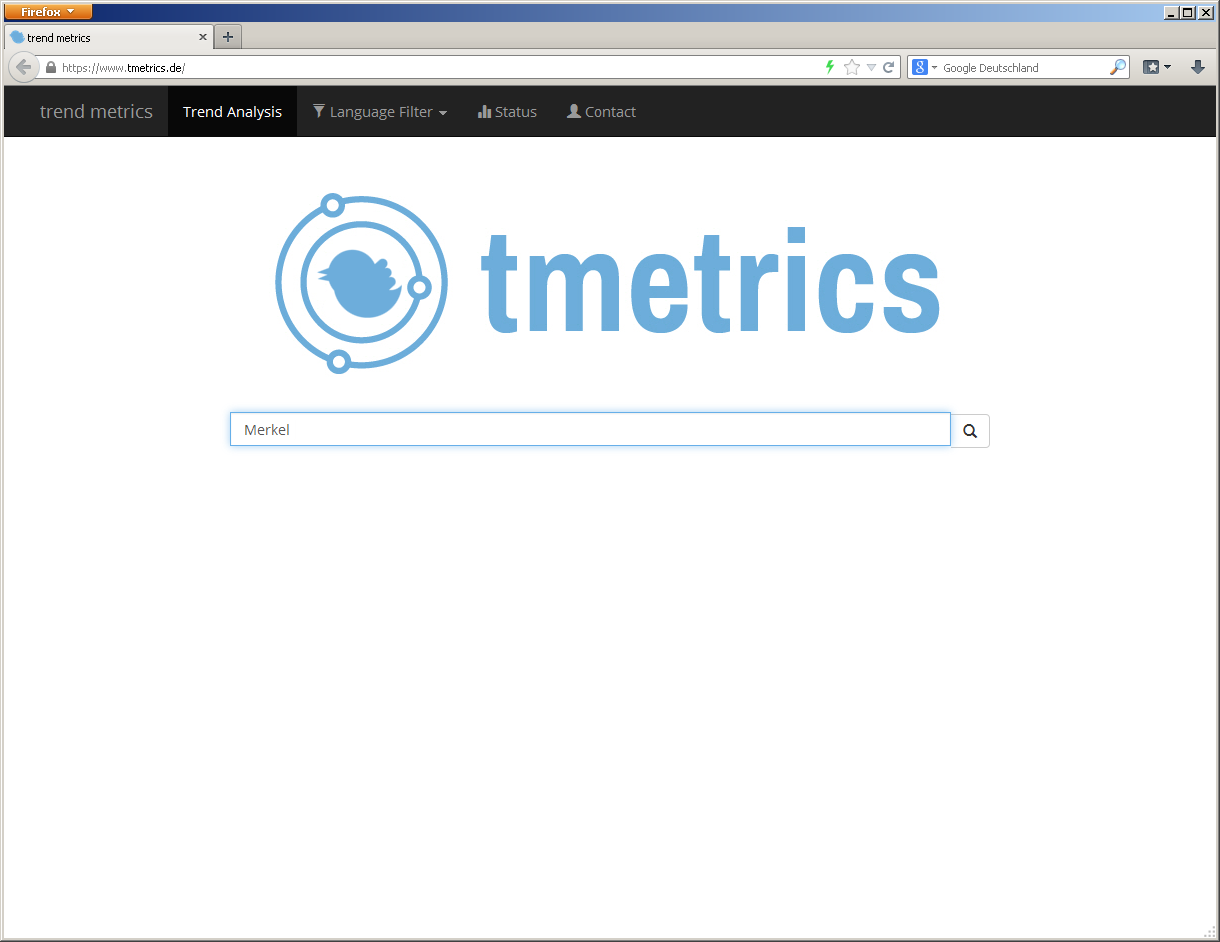
\includegraphics[width=0.926\textwidth]{../img/shots/01.png}
\end{frame}

\begin{frame}
    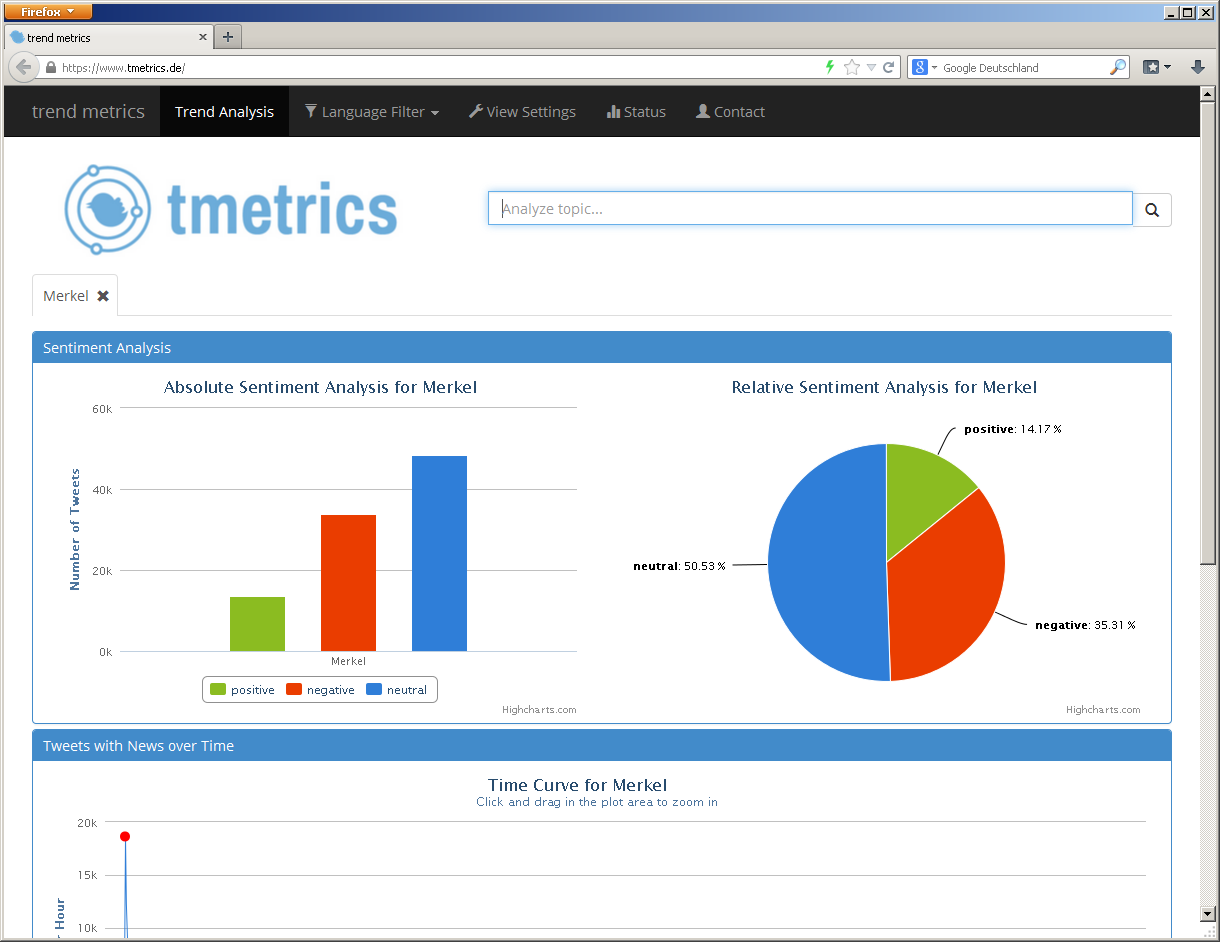
\includegraphics[width=0.926\textwidth]{../img/shots/02.png}
\end{frame}

\begin{frame}
    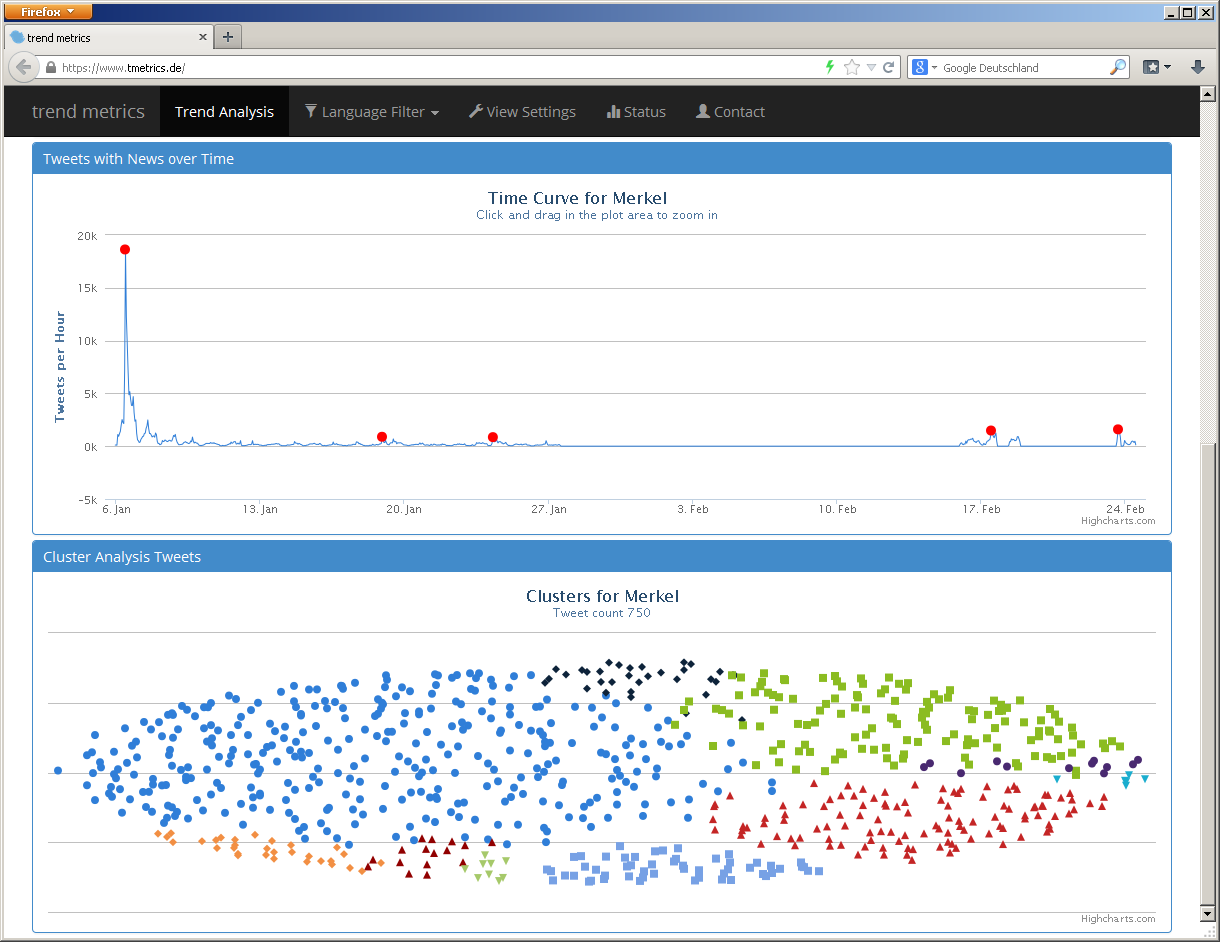
\includegraphics[width=0.926\textwidth]{../img/shots/03.png}
\end{frame}

\begin{frame}
    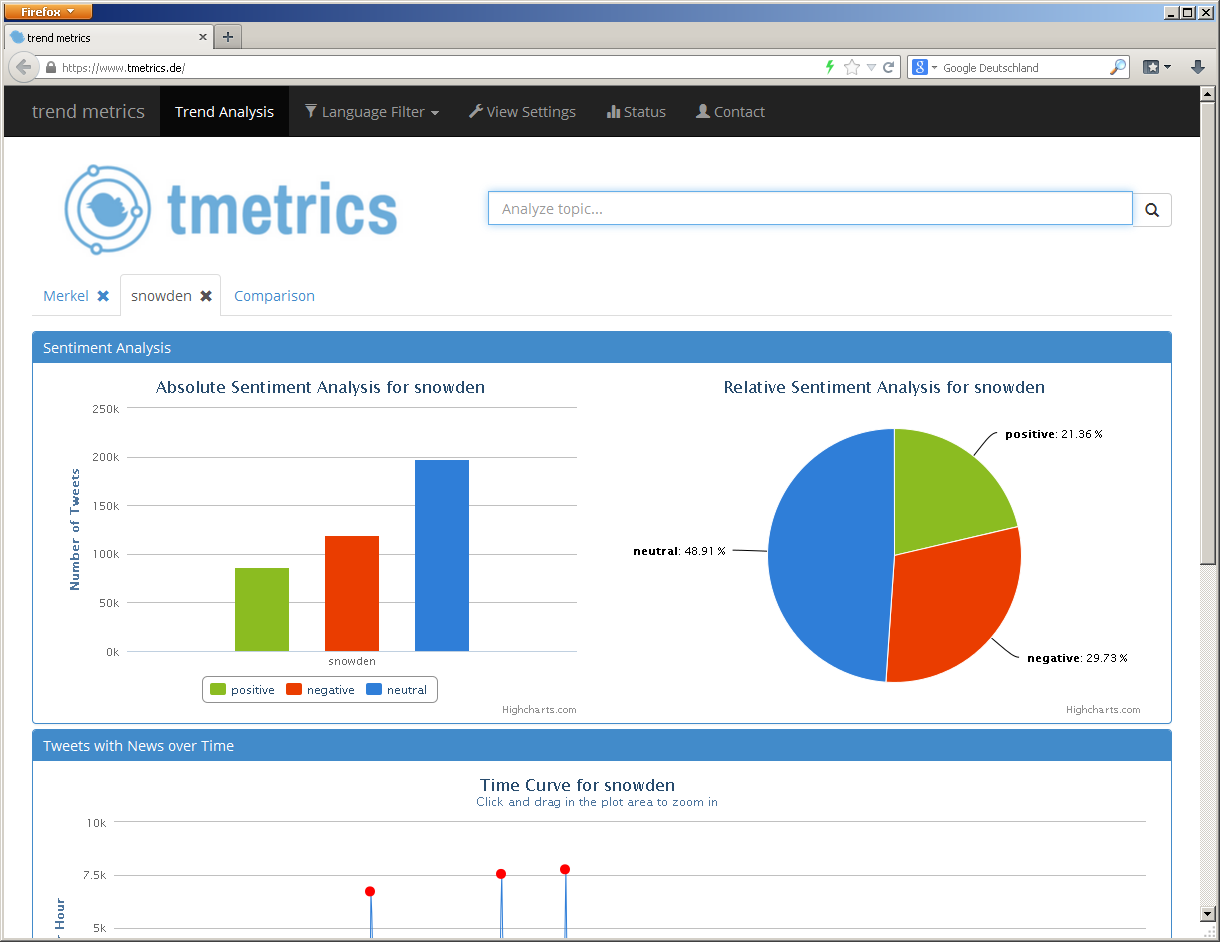
\includegraphics[width=0.926\textwidth]{../img/shots/04.png}
\end{frame}

\begin{frame}
    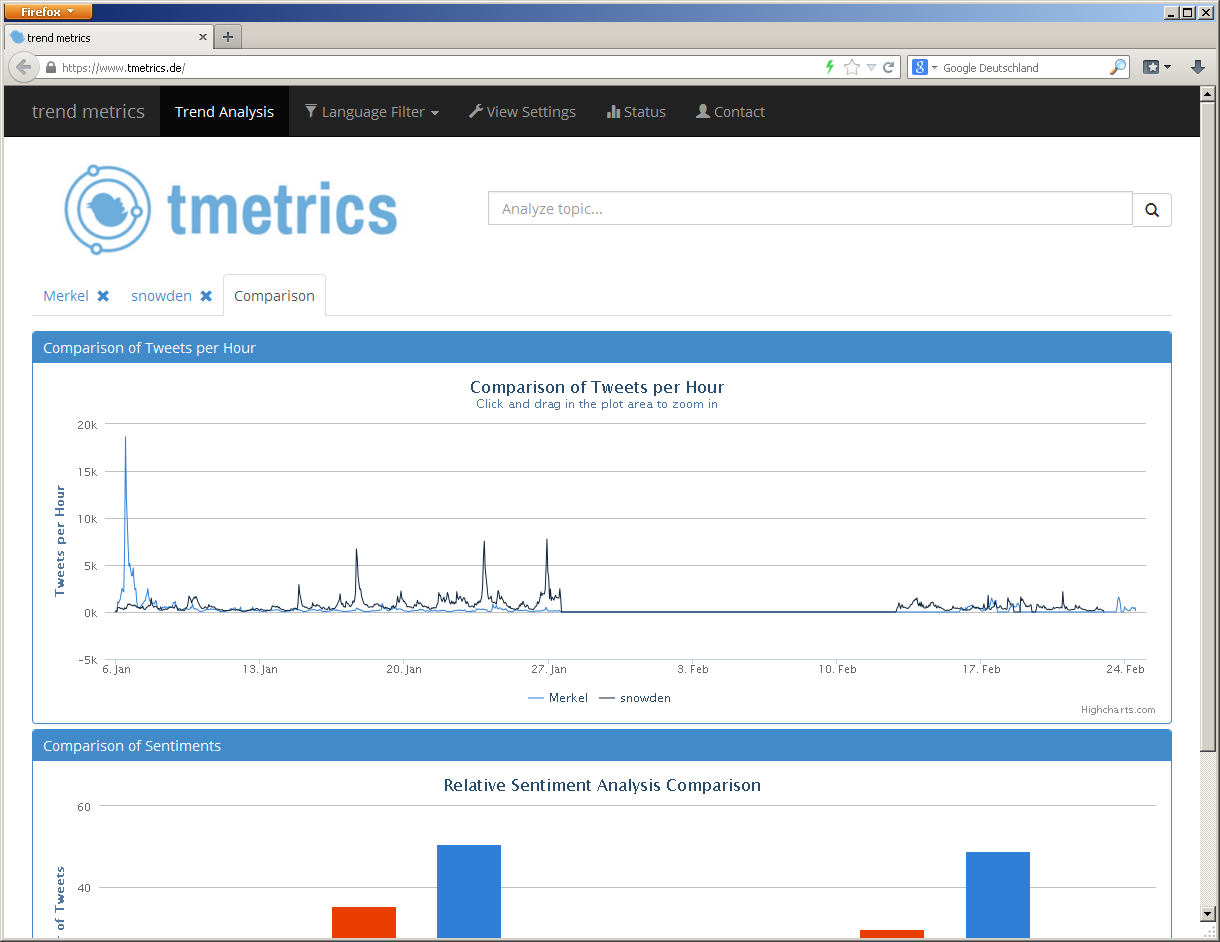
\includegraphics[width=0.926\textwidth]{../img/shots/06.png}
\end{frame}

\begin{frame}
    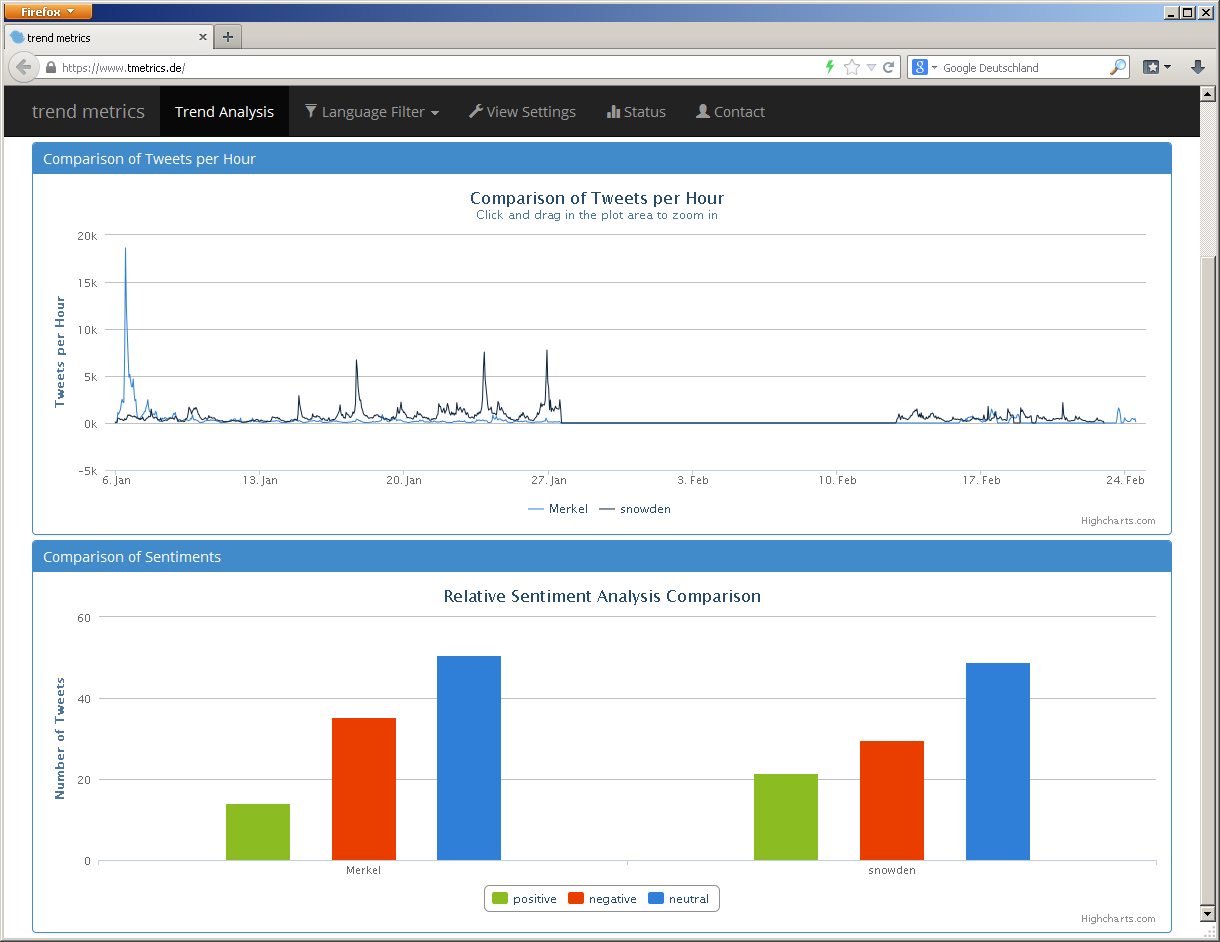
\includegraphics[width=0.926\textwidth]{../img/shots/07.png}
\end{frame}

\begin{frame}{Aufbau - Frontend}
    \begin{itemize}
        \item Einfach und intuitiv zu bedienen
        \item Reiter und Zoom sind bekannte Bedienkonzepte
        \item Anzeigebereich nicht überladen, sondern übersichtlich gehalten
        \item Weitere Details zur Funktionalität folgen in der Demonstration
    \end{itemize}
\end{frame}


\section{Die einzelnen Module}
\subsection{Daemon}
  
\begin{frame}{Module - Daemon - Aufgaben}
	\begin{itemize}
		\item Sammeln von Tweets zu Begriffen
		\item Speichern von Tweets in der Datenbank
		\item Verwendung der Twitter API
	\end{itemize}
	
	\pause
	
	\begin{center}
		\begin{tabular}{ccccc}
		
\includegraphics[width=0.1\textwidth]{../img/daemon/Database.png} &  $\leftrightarrow$ & 
\includegraphics[width=0.1\textwidth]{../img/daemon/java.png} & $\leftrightarrow$ &  
\includegraphics[width=0.1\textwidth]{../img/daemon/Twitter_logo_blue.pdf} \\
		Datenbank & & Daemon & & TwitterAPI \\
		\end{tabular}

	\end{center}
	
	\pause
	
	\begin{itemize}
		\item Sentiment berechnen
	\end{itemize}
	
\end{frame}

\begin{frame}{Module - Daemon - Twitter-API}
	\begin{itemize}
		\item Twitter hat eine offizielle API
		\item Search-API: REST-Anfragen liefern JSON-Objekte
		\item Twitter API unterliegt Restriktionen % (Rate Limit pro Profil, Art, wie Tweets abgefragt werden)
		\item Kommunikation mit Twitter über Twitter4J
	\end{itemize}
\end{frame}

\begin{frame}{Module - Daemon - Suchstrategie}
	\begin{itemize}
		\item Suche zu Suchbegriff immer rückwärts
		\item Suche: ältester Tweet ist Beschränkung für nächste Anfrage
		\item Tweets sind zeitlich sortiert
		\pause
		\item Keine älteren Tweets mehr: Startzeitpunkt auf jetzt setzen
		\item Ab diesem Zeitpunkt wird erneut rückwärts gesucht
	\end{itemize}
\end{frame}

\begin{frame}[t]{Module - Daemon - Suchstrategie}
	\begin{center}
	\includegraphics<1>[width=0.9\textwidth]{../img/daemon/SearchStrategy1.pdf}
	\includegraphics<2>[width=0.9\textwidth]{../img/daemon/SearchStrategy1_5.pdf}
	\includegraphics<3>[width=0.9\textwidth]{../img/daemon/SearchStrategy2.pdf}
	\includegraphics<4>[width=0.9\textwidth]{../img/daemon/SearchStrategy3.pdf}
	\includegraphics<5>[width=0.9\textwidth]{../img/daemon/SearchStrategy4.pdf}
	\end{center}
\end{frame}

\begin{frame}{Module - Daemon - Parallele Suche}
	\begin{itemize}
		\item Parallele Suche: mehr Tweets in kürzer Zeit finden
		\item Idee: mehrere Profile nutzen (Multi-Threading)
		\item Daemon als Master-Worker-Architektur realisieren
	\end{itemize}
\end{frame}

\begin{frame}{Module - Daemon - Scheduling der Suchbegriffe}
	\begin{itemize}
		\item Wie teilt man die Suchbegriffe auf?
		\item Short-Terms, kaum neue Tweets
		\item Long-Terms, viele neuen Tweets
		\item Worker erhält sowohl Short- als auch Long-Terms
	\end{itemize}
\end{frame}

%\begin{frame}[t]{Architektur}
%	\vspace{-1cm}
%	\begin{center}
%	\includegraphics<1>[height=\textheight]{../img/daemon/DataFlow1.pdf}
%	\includegraphics<2>[height=\textheight]{../img/daemon/DataFlow2.pdf}
%	\includegraphics<3>[height=\textheight]{../img/daemon/DataFlow3.pdf}
%	\includegraphics<4>[height=\textheight]{../img/daemon/DataFlow4.pdf}
%%	\includegraphics<5>[height=\textheight]{../img/daemon/DataFlow1.pdf}
%	\end{center}
%\end{frame}


\begin{frame}{Module - Daemon - Erfahrungen}
	\begin{itemize}
		\item Multi-Threading ist komplex
		\item Probleme mit dem Speicherverbrauch der JVM
		\item Konsistenz der verschiedenen Teile komplex
	\end{itemize}
\end{frame}

  \subsection{Clustering}
  % \begin{frame}{Module - Clustering - Grundidee}
% %Grundidee:
% \begin{itemize}
%  \item Tweets visuell als Punkte darstellen,
%  \item Tweets nach Themen gruppieren,
% % 	damit man einen Eindruck bekommt 
% %        welche unterschiedliche ``Meinungen'' es zu einem Begriff gibt oder welche 
% %        Hashtags zusammen verwendet werden,
%  \item die Distanzen zeigen die Unterschiede.
% %  zwischen den dargestellten Punkten sollen suggerieren, wie 
% %        ähnlich bzw. unterschiedlich sich die betroffenen Tweets sind (zumindest grob).
% \end{itemize}
% \end{frame}


\begin{frame}{Module - Clustering - Grundidee}
%Beispiel:\\
\begin{tikzpicture}[y=\textwidth/100,x=\textwidth/44, background rectangle/.style={draw=black, thick, fill=yellow!10,},show background rectangle]
\def\marRad{0.5mm}
\definecolor{color0}{rgb}{0.73,0.10,0.41}
\definecolor{color1}{rgb}{0.41,0.21,0.04}
\definecolor{color2}{rgb}{0.33,0.66,0.97}
\definecolor{color3}{rgb}{0.71,0.00,0.15}
\definecolor{color4}{rgb}{0.96,0.16,0.94}
\definecolor{color5}{rgb}{0.55,0.95,0.91}
\definecolor{color6}{rgb}{0.94,0.49,0.40}

\path[fill=color0,draw=color0,mark size=\marRad, mark=*] plot coordinates {(11.03, 13.77)};
\path[fill=color0,draw=color0,mark size=\marRad, mark=*] plot coordinates {(10.76, 8.68)};
\path[fill=color0,draw=color0,mark size=\marRad, mark=*] plot coordinates {(10.76, 7.31)};
\path[fill=color0,draw=color0,mark size=\marRad, mark=*] plot coordinates {(14.14, 10.17)};
\path[fill=color0,draw=color0,mark size=\marRad, mark=*] plot coordinates {(10.55, 10.86)};
\path[fill=color0,draw=color0,mark size=\marRad, mark=*] plot coordinates {(10.40, 10.60)};
\path[fill=color0,draw=color0,mark size=\marRad, mark=*] plot coordinates {(10.28, 10.79)};
\path[fill=color0,draw=color0,mark size=\marRad, mark=*] plot coordinates {(9.16, 12.33)};
\path[fill=color0,draw=color0,mark size=\marRad, mark=*] plot coordinates {(10.02, 10.47)};
\path[fill=color0,draw=color0,mark size=\marRad, mark=*] plot coordinates {(10.01, 10.02)};
\path[fill=color0,draw=color0,mark size=\marRad, mark=*] plot coordinates {(12.57, 11.35)};
\path[fill=color0,draw=color0,mark size=\marRad, mark=*] plot coordinates {(11.40, 14.80)};
\path[fill=color0,draw=color0,mark size=\marRad, mark=*] plot coordinates {(11.14, 10.08)};
\path[fill=color0,draw=color0,mark size=\marRad, mark=*] plot coordinates {(8.46, 7.54)};
\path[fill=color0,draw=color0,mark size=\marRad, mark=*] plot coordinates {(6.78, 10.53)};
\path[fill=color0,draw=color0,mark size=\marRad, mark=*] plot coordinates {(10.01, 10.41)};
\path[fill=color0,draw=color0,mark size=\marRad, mark=*] plot coordinates {(11.13, 9.48)};
\path[fill=color0,draw=color0,mark size=\marRad, mark=*] plot coordinates {(9.65, 6.69)};
\path[fill=color0,draw=color0,mark size=\marRad, mark=*] plot coordinates {(11.88, 11.76)};
\path[fill=color0,draw=color0,mark size=\marRad, mark=*] plot coordinates {(7.51, 6.45)};
\path[fill=color0,draw=color0,mark size=\marRad, mark=*] plot coordinates {(12.79, 5.19)};
\path[fill=color0,draw=color0,mark size=\marRad, mark=*] plot coordinates {(11.52, 9.43)};
\path[fill=color0,draw=color0,mark size=\marRad, mark=*] plot coordinates {(10.00, 10.00)};
\path[fill=color0,draw=color0,mark size=\marRad, mark=*] plot coordinates {(10.19, 9.88)};
\path[fill=color0,draw=color0,mark size=\marRad, mark=*] plot coordinates {(5.49, 12.16)};
\path[fill=color0,draw=color0,mark size=2*\marRad, mark=*] plot coordinates {(12.58, 3.24)};
\path[fill=color0,draw=color0,mark size=\marRad, mark=*] plot coordinates {(11.15, 10.37)};
\path[fill=color0,draw=color0,mark size=\marRad, mark=*] plot coordinates {(11.28, 10.47)};
\path[fill=color0,draw=color0,mark size=\marRad, mark=*] plot coordinates {(9.68, 9.02)};
\path[fill=color0,draw=color0,mark size=\marRad, mark=*] plot coordinates {(10.95, 13.26)};
\path[fill=color0,draw=color0,mark size=\marRad, mark=*] plot coordinates {(9.72, 8.21)};
\path[fill=color0,draw=color0,mark size=\marRad, mark=*] plot coordinates {(12.04, 9.78)};
\path[fill=color0,draw=color0,mark size=\marRad, mark=*] plot coordinates {(10.55, 10.90)};
\path[fill=color0,draw=color0,mark size=\marRad, mark=*] plot coordinates {(9.24, 9.11)};
\path[fill=color0,draw=color0,mark size=\marRad, mark=*] plot coordinates {(10.17, 10.60)};
\path[fill=color0,draw=color0,mark size=\marRad, mark=*] plot coordinates {(9.86, 9.20)};
\path[fill=color0,draw=color0,mark size=\marRad, mark=*] plot coordinates {(10.01, 10.01)};
\path[fill=color0,draw=color0,mark size=\marRad, mark=*] plot coordinates {(9.80, 9.22)};
\path[fill=color0,draw=color0,mark size=\marRad, mark=*] plot coordinates {(9.80, 9.82)};
\path[fill=color0,draw=color0,mark size=\marRad, mark=*] plot coordinates {(10.31, 9.96)};
\path[fill=color0,draw=color0,mark size=\marRad, mark=*] plot coordinates {(7.99, 9.64)};
\path[fill=color0,draw=color0,mark size=\marRad, mark=*] plot coordinates {(9.50, 9.67)};
\path[fill=color0,draw=color0,mark size=\marRad, mark=*] plot coordinates {(8.11, 8.55)};
\path[fill=color0,draw=color0,mark size=\marRad, mark=*] plot coordinates {(8.30, 12.36)};
\path[fill=color0,draw=color0,mark size=\marRad, mark=*] plot coordinates {(11.11, 5.92)};
\path[fill=color0,draw=color0,mark size=\marRad, mark=*] plot coordinates {(12.04, 8.00)};
\path[fill=color0,draw=color0,mark size=\marRad, mark=*] plot coordinates {(7.23, 12.75)};
\path[fill=color0,draw=color0,mark size=\marRad, mark=*] plot coordinates {(10.16, 8.78)};
\path[fill=color0,draw=color0,mark size=\marRad, mark=*] plot coordinates {(10.80, 10.23)};
\path[fill=color0,draw=color0,mark size=\marRad, mark=*] plot coordinates {(8.65, 10.37)};
\path[fill=color0,draw=color0,mark size=\marRad, mark=*] plot coordinates {(11.50, 10.68)};
\path[fill=color0,draw=color0,mark size=\marRad, mark=*] plot coordinates {(9.83, 9.72)};
\path[fill=color0,draw=color0,mark size=\marRad, mark=*] plot coordinates {(10.01, 10.86)};
\path[fill=color0,draw=color0,mark size=\marRad, mark=*] plot coordinates {(10.14, 10.52)};
\path[fill=color0,draw=color0,mark size=\marRad, mark=*] plot coordinates {(11.62, 6.29)};
\path[fill=color0,draw=color0,mark size=\marRad, mark=*] plot coordinates {(12.65, 10.41)};
\path[fill=color0,draw=color0,mark size=\marRad, mark=*] plot coordinates {(11.93, 9.55)};
\path[fill=color0,draw=color0,mark size=\marRad, mark=*] plot coordinates {(7.67, 5.26)};
\path[fill=color0,draw=color0,mark size=\marRad, mark=*] plot coordinates {(9.90, 7.58)};
\path[fill=color0,draw=color0,mark size=\marRad, mark=*] plot coordinates {(12.67, 8.72)};
\path[fill=color0,draw=color0,mark size=\marRad, mark=*] plot coordinates {(12.11, 11.76)};
\path[fill=color0,draw=color0,mark size=\marRad, mark=*] plot coordinates {(10.68, 5.64)};
\path[fill=color0,draw=color0,mark size=\marRad, mark=*] plot coordinates {(10.61, 10.66)};
\path[fill=color0,draw=color0,mark size=\marRad, mark=*] plot coordinates {(11.60, 9.23)};
\path[fill=color0,draw=color0,mark size=\marRad, mark=*] plot coordinates {(8.99, 8.45)};
\path[fill=color0,draw=color0,mark size=\marRad, mark=*] plot coordinates {(11.50, 10.41)};
\path[fill=color0,draw=color0,mark size=\marRad, mark=*] plot coordinates {(10.31, 11.31)};
\path[fill=color0,draw=color0,mark size=\marRad, mark=*] plot coordinates {(12.44, 12.02)};
\path[fill=color0,draw=color0,mark size=\marRad, mark=*] plot coordinates {(12.77, 8.62)};
\path[fill=color0,draw=color0,mark size=\marRad, mark=*] plot coordinates {(7.71, 11.65)};
\path[fill=color0,draw=color0,mark size=\marRad, mark=*] plot coordinates {(10.29, 6.66)};
\path[fill=color0,draw=color0,mark size=\marRad, mark=*] plot coordinates {(10.82, 8.34)};
\path[fill=color0,draw=color0,mark size=\marRad, mark=*] plot coordinates {(13.01, 13.26)};
\path[fill=color0,draw=color0,mark size=\marRad, mark=*] plot coordinates {(2.71, 8.52)};
\path[fill=color0,draw=color0,mark size=\marRad, mark=*] plot coordinates {(10.26, 11.31)};
\path[fill=color0,draw=color0,mark size=\marRad, mark=*] plot coordinates {(10.80, 5.47)};
\path[fill=color0,draw=color0,mark size=\marRad, mark=*] plot coordinates {(8.26, 10.37)};
\path[fill=color0,draw=color0,mark size=\marRad, mark=*] plot coordinates {(12.36, 9.95)};
\path[fill=color0,draw=color0,mark size=\marRad, mark=*] plot coordinates {(7.35, 7.17)};
\path[fill=color0,draw=color0,mark size=\marRad, mark=*] plot coordinates {(9.92, 9.19)};
\path[fill=color0,draw=color0,mark size=\marRad, mark=*] plot coordinates {(5.60, 8.39)};
\path[fill=color0,draw=color0,mark size=\marRad, mark=*] plot coordinates {(10.00, 12.17)};
\path[fill=color0,draw=color0,mark size=\marRad, mark=*] plot coordinates {(10.16, 9.04)};
\path[fill=color0,draw=color0,mark size=\marRad, mark=*] plot coordinates {(10.03, 10.52)};
\path[fill=color0,draw=color0,mark size=\marRad, mark=*] plot coordinates {(8.47, 12.80)};
\path[fill=color0,draw=color0,mark size=\marRad, mark=*] plot coordinates {(10.44, 10.32)};
\path[fill=color0,draw=color0,mark size=\marRad, mark=*] plot coordinates {(12.25, 10.98)};
\path[fill=color0,draw=color0,mark size=\marRad, mark=*] plot coordinates {(6.76, 11.33)};
\path[fill=color0,draw=color0,mark size=\marRad, mark=*] plot coordinates {(10.63, 8.22)};
\path[fill=color0,draw=color0,mark size=\marRad, mark=*] plot coordinates {(11.52, 8.42)};
\path[fill=color0,draw=color0,mark size=\marRad, mark=*] plot coordinates {(9.29, 10.60)};
\path[fill=color0,draw=color0,mark size=\marRad, mark=*] plot coordinates {(9.92, 10.79)};
\path[fill=color0,draw=color0,mark size=\marRad, mark=*] plot coordinates {(9.70, 9.85)};
\path[fill=color0,draw=color0,mark size=\marRad, mark=*] plot coordinates {(9.91, 9.92)};
\path[fill=color0,draw=color0,mark size=\marRad, mark=*] plot coordinates {(11.80, 11.60)};
\path[fill=color0,draw=color0,mark size=\marRad, mark=*] plot coordinates {(10.93, 12.40)};
\path[fill=color0,draw=color0,mark size=\marRad, mark=*] plot coordinates {(9.17, 8.55)};
\path[fill=color0,draw=color0,mark size=\marRad, mark=*] plot coordinates {(12.50, 11.69)};
\path[fill=color0,draw=color0,mark size=\marRad, mark=*] plot coordinates {(7.99, 12.80)};
\path[fill=color0,draw=color0,mark size=\marRad, mark=*] plot coordinates {(10.16, 10.05)};
\path[fill=color0,draw=color0,mark size=\marRad, mark=*] plot coordinates {(7.97, 8.82)};
\path[fill=color0,draw=color0,mark size=\marRad, mark=*] plot coordinates {(7.26, 12.93)};
\path[fill=color0,draw=color0,mark size=\marRad, mark=*] plot coordinates {(10.13, 10.84)};
\path[fill=color0,draw=color0,mark size=\marRad, mark=*] plot coordinates {(9.67, 10.12)};
\path[fill=color0,draw=color0,mark size=\marRad, mark=*] plot coordinates {(11.11, 7.46)};
\path[fill=color0,draw=color0,mark size=\marRad, mark=*] plot coordinates {(8.20, 7.34)};
\path[fill=color0,draw=color0,mark size=\marRad, mark=*] plot coordinates {(11.18, 10.38)};
\path[fill=color0,draw=color0,mark size=\marRad, mark=*] plot coordinates {(14.76, 10.67)};
\path[fill=color0,draw=color0,mark size=\marRad, mark=*] plot coordinates {(7.77, 8.49)};
\path[fill=color0,draw=color0,mark size=\marRad, mark=*] plot coordinates {(12.77, 9.27)};
\path[fill=color0,draw=color0,mark size=\marRad, mark=*] plot coordinates {(9.69, 10.06)};
\path[fill=color0,draw=color0,mark size=\marRad, mark=*] plot coordinates {(8.05, 12.68)};
\path[fill=color0,draw=color0,mark size=\marRad, mark=*] plot coordinates {(10.11, 9.76)};
\path[fill=color0,draw=color0,mark size=\marRad, mark=*] plot coordinates {(10.00, 10.35)};
\path[fill=color0,draw=color0,mark size=\marRad, mark=*] plot coordinates {(9.93, 10.65)};
\path[fill=color0,draw=color0,mark size=\marRad, mark=*] plot coordinates {(9.46, 7.94)};
\path[fill=color0,draw=color0,mark size=\marRad, mark=*] plot coordinates {(13.07, 8.75)};
\path[fill=color0,draw=color0,mark size=\marRad, mark=*] plot coordinates {(11.52, 11.02)};
\path[fill=color0,draw=color0,mark size=\marRad, mark=*] plot coordinates {(10.04, 8.83)};
\path[fill=color0,draw=color0,mark size=\marRad, mark=*] plot coordinates {(9.13, 8.94)};
\path[fill=color0,draw=color0,mark size=\marRad, mark=*] plot coordinates {(8.46, 10.38)};
\path[fill=color0,draw=color0,mark size=\marRad, mark=*] plot coordinates {(11.62, 11.51)};
\path[fill=color0,draw=color0,mark size=\marRad, mark=*] plot coordinates {(10.17, 10.06)};
\path[fill=color0,draw=color0,mark size=\marRad, mark=*] plot coordinates {(6.06, 8.44)};
\path[fill=color0,draw=color0,mark size=\marRad, mark=*] plot coordinates {(9.45, 10.51)};
\path[fill=color0,draw=color0,mark size=\marRad, mark=*] plot coordinates {(12.02, 10.81)};
\path[fill=color0,draw=color0,mark size=\marRad, mark=*] plot coordinates {(10.81, 7.08)};
\path[fill=color0,draw=color0,mark size=\marRad, mark=*] plot coordinates {(11.19, 8.95)};
\path[fill=color0,draw=color0,mark size=\marRad, mark=*] plot coordinates {(10.41, 10.92)};
\path[fill=color0,draw=color0,mark size=\marRad, mark=*] plot coordinates {(7.36, 13.76)};
\path[fill=color0,draw=color0,mark size=\marRad, mark=*] plot coordinates {(7.73, 10.49)};
\path[fill=color0,draw=color0,mark size=\marRad, mark=*] plot coordinates {(10.54, 8.46)};
\path[fill=color0,draw=color0,mark size=\marRad, mark=*] plot coordinates {(7.95, 10.51)};
\path[fill=color0,draw=color0,mark size=\marRad, mark=*] plot coordinates {(9.99, 9.90)};
\path[fill=color0,draw=color0,mark size=\marRad, mark=*] plot coordinates {(3.57, 7.18)};
\path[fill=color0,draw=color0,mark size=\marRad, mark=*] plot coordinates {(7.80, 8.21)};
\path[fill=color0,draw=color0,mark size=\marRad, mark=*] plot coordinates {(11.94, 12.06)};
\path[fill=color0,draw=color0,mark size=\marRad, mark=*] plot coordinates {(8.89, 10.89)};
\path[fill=color0,draw=color0,mark size=\marRad, mark=*] plot coordinates {(10.23, 10.42)};
\path[fill=color0,draw=color0,mark size=\marRad, mark=*] plot coordinates {(12.61, 10.29)};
\path[fill=color0,draw=color0,mark size=\marRad, mark=*] plot coordinates {(9.80, 10.18)};
\path[fill=color0,draw=color0,mark size=\marRad, mark=*] plot coordinates {(10.97, 11.83)};
\path[fill=color0,draw=color0,mark size=\marRad, mark=*] plot coordinates {(8.04, 11.96)};
\path[fill=color0,draw=color0,mark size=\marRad, mark=*] plot coordinates {(10.14, 9.91)};
\path[fill=color0,draw=color0,mark size=\marRad, mark=*] plot coordinates {(10.65, 11.04)};
\path[fill=color0,draw=color0,mark size=\marRad, mark=*] plot coordinates {(10.12, 15.00)};
\path[fill=color0,draw=color0,mark size=\marRad, mark=*] plot coordinates {(11.77, 10.99)};
\path[fill=color0,draw=color0,mark size=\marRad, mark=*] plot coordinates {(9.49, 13.77)};
\path[fill=color0,draw=color0,mark size=\marRad, mark=*] plot coordinates {(12.78, 6.93)};
\path[fill=color0,draw=color0,mark size=\marRad, mark=*] plot coordinates {(7.95, 7.76)};
\path[fill=color0,draw=color0,mark size=\marRad, mark=*] plot coordinates {(8.76, 8.44)};
\path[fill=color0,draw=color0,mark size=\marRad, mark=*] plot coordinates {(10.74, 10.34)};
\path[fill=color0,draw=color0,mark size=\marRad, mark=*] plot coordinates {(5.09, 9.05)};
\path[fill=color0,draw=color0,mark size=\marRad, mark=*] plot coordinates {(12.34, 8.57)};
\path[fill=color0,draw=color0,mark size=\marRad, mark=*] plot coordinates {(9.20, 10.42)};
\path[fill=color0,draw=color0,mark size=\marRad, mark=*] plot coordinates {(9.07, 10.02)};
\path[fill=color0,draw=color0,mark size=\marRad, mark=*] plot coordinates {(8.76, 9.30)};
\path[fill=color0,draw=color0,mark size=\marRad, mark=*] plot coordinates {(8.18, 10.62)};
\path[fill=color0,draw=color0,mark size=\marRad, mark=*] plot coordinates {(12.94, 15.26)};
\path[fill=color0,draw=color0,mark size=\marRad, mark=*] plot coordinates {(10.91, 7.79)};
\path[fill=color0,draw=color0,mark size=\marRad, mark=*] plot coordinates {(9.74, 8.57)};
\path[fill=color0,draw=color0,mark size=\marRad, mark=*] plot coordinates {(9.18, 9.89)};
\path[fill=color0,draw=color0,mark size=\marRad, mark=*] plot coordinates {(8.88, 9.76)};
\path[fill=color0,draw=color0,mark size=\marRad, mark=*] plot coordinates {(9.82, 11.65)};
\path[fill=color0,draw=color0,mark size=\marRad, mark=*] plot coordinates {(12.46, 11.08)};
\path[fill=color0,draw=color0,mark size=\marRad, mark=*] plot coordinates {(7.90, 9.75)};
\path[fill=color0,draw=color0,mark size=\marRad, mark=*] plot coordinates {(9.39, 6.64)};
\path[fill=color0,draw=color0,mark size=\marRad, mark=*] plot coordinates {(9.68, 9.94)};
\path[fill=color0,draw=color0,mark size=\marRad, mark=*] plot coordinates {(8.64, 11.70)};
\path[fill=color0,draw=color0,mark size=\marRad, mark=*] plot coordinates {(13.24, 8.50)};
\path[fill=color0,draw=color0,mark size=\marRad, mark=*] plot coordinates {(6.40, 10.78)};
\path[fill=color0,draw=color0,mark size=\marRad, mark=*] plot coordinates {(10.68, 8.50)};
\path[fill=color0,draw=color0,mark size=\marRad, mark=*] plot coordinates {(10.01, 10.02)};
\path[fill=color0,draw=color0,mark size=\marRad, mark=*] plot coordinates {(10.15, 8.76)};
\path[fill=color0,draw=color0,mark size=\marRad, mark=*] plot coordinates {(8.43, 11.54)};
\path[fill=color0,draw=color0,mark size=\marRad, mark=*] plot coordinates {(9.93, 10.43)};
\path[fill=color0,draw=color0,mark size=\marRad, mark=*] plot coordinates {(10.01, 10.00)};
\path[fill=color0,draw=color0,mark size=\marRad, mark=*] plot coordinates {(9.59, 4.88)};
\path[fill=color0,draw=color0,mark size=\marRad, mark=*] plot coordinates {(10.31, 9.16)};
\path[fill=color0,draw=color0,mark size=\marRad, mark=*] plot coordinates {(11.83, 11.48)};
\path[fill=color0,draw=color0,mark size=\marRad, mark=*] plot coordinates {(6.51, 8.06)};
\path[fill=color0,draw=color0,mark size=\marRad, mark=*] plot coordinates {(10.41, 10.10)};
\path[fill=color0,draw=color0,mark size=\marRad, mark=*] plot coordinates {(10.75, 10.50)};
\path[fill=color0,draw=color0,mark size=\marRad, mark=*] plot coordinates {(9.05, 9.59)};
\path[fill=color0,draw=color0,mark size=\marRad, mark=*] plot coordinates {(6.64, 14.04)};
\path[fill=color0,draw=color0,mark size=\marRad, mark=*] plot coordinates {(10.66, 10.08)};
\path[fill=color0,draw=color0,mark size=\marRad, mark=*] plot coordinates {(9.38, 8.28)};
\path[fill=color0,draw=color0,mark size=\marRad, mark=*] plot coordinates {(8.08, 8.74)};
\path[fill=color0,draw=color0,mark size=\marRad, mark=*] plot coordinates {(12.77, 9.77)};
\path[fill=color0,draw=color0,mark size=\marRad, mark=*] plot coordinates {(10.80, 9.54)};
\path[fill=color0,draw=color0,mark size=\marRad, mark=*] plot coordinates {(9.82, 10.37)};
\path[fill=color0,draw=color0,mark size=\marRad, mark=*] plot coordinates {(6.11, 9.61)};
\path[fill=color0,draw=color0,mark size=\marRad, mark=*] plot coordinates {(7.15, 9.67)};
\path[fill=color0,draw=color0,mark size=\marRad, mark=*] plot coordinates {(9.56, 10.12)};
\path[fill=color0,draw=color0,mark size=\marRad, mark=*] plot coordinates {(7.95, 10.11)};
\path[fill=color0,draw=color0,mark size=\marRad, mark=*] plot coordinates {(10.36, 9.52)};
\path[fill=color0,draw=color0,mark size=\marRad, mark=*] plot coordinates {(13.15, 11.54)};
\path[fill=color0,draw=color0,mark size=\marRad, mark=*] plot coordinates {(10.06, 9.72)};
\path[fill=color0,draw=color0,mark size=\marRad, mark=*] plot coordinates {(9.53, 10.75)};
\path[fill=color0,draw=color0,mark size=\marRad, mark=*] plot coordinates {(6.52, 9.99)};
\path[fill=color1,draw=color1,mark size=\marRad, mark=square*] plot coordinates {(31.03, 13.77)};
\path[fill=color1,draw=color1,mark size=\marRad, mark=square*] plot coordinates {(30.76, 8.68)};
\path[fill=color1,draw=color1,mark size=\marRad, mark=square*] plot coordinates {(30.76, 7.31)};
\path[fill=color1,draw=color1,mark size=\marRad, mark=square*] plot coordinates {(34.14, 10.17)};
\path[fill=color1,draw=color1,mark size=\marRad, mark=square*] plot coordinates {(30.55, 10.86)};
\path[fill=color1,draw=color1,mark size=\marRad, mark=square*] plot coordinates {(30.40, 10.60)};
\path[fill=color1,draw=color1,mark size=\marRad, mark=square*] plot coordinates {(30.28, 10.79)};
\path[fill=color1,draw=color1,mark size=\marRad, mark=square*] plot coordinates {(29.16, 12.33)};
\path[fill=color1,draw=color1,mark size=\marRad, mark=square*] plot coordinates {(30.02, 10.47)};
\path[fill=color1,draw=color1,mark size=\marRad, mark=square*] plot coordinates {(30.01, 10.02)};
\path[fill=color1,draw=color1,mark size=\marRad, mark=square*] plot coordinates {(32.57, 11.35)};
\path[fill=color1,draw=color1,mark size=\marRad, mark=square*] plot coordinates {(31.40, 14.80)};
\path[fill=color1,draw=color1,mark size=\marRad, mark=square*] plot coordinates {(31.14, 10.08)};
\path[fill=color1,draw=color1,mark size=\marRad, mark=square*] plot coordinates {(28.46, 7.54)};
\path[fill=color1,draw=color1,mark size=\marRad, mark=square*] plot coordinates {(26.78, 10.53)};
\path[fill=color1,draw=color1,mark size=\marRad, mark=square*] plot coordinates {(30.01, 10.41)};
\path[fill=color1,draw=color1,mark size=\marRad, mark=square*] plot coordinates {(31.13, 9.48)};
\path[fill=color1,draw=color1,mark size=\marRad, mark=square*] plot coordinates {(29.65, 6.69)};
\path[fill=color1,draw=color1,mark size=\marRad, mark=square*] plot coordinates {(31.88, 11.76)};
\path[fill=color1,draw=color1,mark size=\marRad, mark=square*] plot coordinates {(27.51, 6.45)};
\path[fill=color1,draw=color1,mark size=\marRad, mark=square*] plot coordinates {(32.79, 5.19)};
\path[fill=color1,draw=color1,mark size=\marRad, mark=square*] plot coordinates {(31.52, 9.43)};
\path[fill=color1,draw=color1,mark size=\marRad, mark=square*] plot coordinates {(30.00, 10.00)};
\path[fill=color1,draw=color1,mark size=\marRad, mark=square*] plot coordinates {(30.19, 9.88)};
\path[fill=color1,draw=color1,mark size=\marRad, mark=square*] plot coordinates {(25.49, 12.16)};
\path[fill=color1,draw=color1,mark size=\marRad, mark=square*] plot coordinates {(32.58, 3.24)};
\path[fill=color1,draw=color1,mark size=\marRad, mark=square*] plot coordinates {(31.15, 10.37)};
\path[fill=color1,draw=color1,mark size=\marRad, mark=square*] plot coordinates {(31.28, 10.47)};
\path[fill=color1,draw=color1,mark size=\marRad, mark=square*] plot coordinates {(29.68, 9.02)};
\path[fill=color1,draw=color1,mark size=\marRad, mark=square*] plot coordinates {(30.95, 13.26)};
\path[fill=color1,draw=color1,mark size=\marRad, mark=square*] plot coordinates {(29.72, 8.21)};
\path[fill=color1,draw=color1,mark size=\marRad, mark=square*] plot coordinates {(32.04, 9.78)};
\path[fill=color1,draw=color1,mark size=\marRad, mark=square*] plot coordinates {(30.55, 10.90)};
\path[fill=color1,draw=color1,mark size=\marRad, mark=square*] plot coordinates {(29.24, 9.11)};
\path[fill=color1,draw=color1,mark size=\marRad, mark=square*] plot coordinates {(30.17, 10.60)};
\path[fill=color1,draw=color1,mark size=\marRad, mark=square*] plot coordinates {(29.86, 9.20)};
\path[fill=color1,draw=color1,mark size=\marRad, mark=square*] plot coordinates {(30.01, 10.01)};
\path[fill=color1,draw=color1,mark size=\marRad, mark=square*] plot coordinates {(29.80, 9.22)};
\path[fill=color1,draw=color1,mark size=\marRad, mark=square*] plot coordinates {(29.80, 9.82)};
\path[fill=color1,draw=color1,mark size=\marRad, mark=square*] plot coordinates {(30.31, 9.96)};
\path[fill=color1,draw=color1,mark size=\marRad, mark=square*] plot coordinates {(27.99, 9.64)};
\path[fill=color1,draw=color1,mark size=\marRad, mark=square*] plot coordinates {(29.50, 9.67)};
\path[fill=color1,draw=color1,mark size=\marRad, mark=square*] plot coordinates {(28.11, 8.55)};
\path[fill=color1,draw=color1,mark size=\marRad, mark=square*] plot coordinates {(28.30, 12.36)};
\path[fill=color1,draw=color1,mark size=\marRad, mark=square*] plot coordinates {(31.11, 5.92)};
\path[fill=color1,draw=color1,mark size=\marRad, mark=square*] plot coordinates {(32.04, 8.00)};
\path[fill=color1,draw=color1,mark size=\marRad, mark=square*] plot coordinates {(27.23, 12.75)};
\path[fill=color1,draw=color1,mark size=\marRad, mark=square*] plot coordinates {(30.16, 8.78)};
\path[fill=color1,draw=color1,mark size=\marRad, mark=square*] plot coordinates {(30.80, 10.23)};
\path[fill=color1,draw=color1,mark size=\marRad, mark=square*] plot coordinates {(28.65, 10.37)};
\path[fill=color1,draw=color1,mark size=\marRad, mark=square*] plot coordinates {(31.50, 10.68)};
\path[fill=color1,draw=color1,mark size=\marRad, mark=square*] plot coordinates {(29.83, 9.72)};
\path[fill=color1,draw=color1,mark size=\marRad, mark=square*] plot coordinates {(30.01, 10.86)};
\path[fill=color1,draw=color1,mark size=\marRad, mark=square*] plot coordinates {(30.14, 10.52)};
\path[fill=color1,draw=color1,mark size=\marRad, mark=square*] plot coordinates {(31.62, 6.29)};
\path[fill=color1,draw=color1,mark size=\marRad, mark=square*] plot coordinates {(32.65, 10.41)};
\path[fill=color1,draw=color1,mark size=\marRad, mark=square*] plot coordinates {(31.93, 9.55)};
\path[fill=color1,draw=color1,mark size=\marRad, mark=square*] plot coordinates {(27.67, 5.26)};
\path[fill=color1,draw=color1,mark size=\marRad, mark=square*] plot coordinates {(29.90, 7.58)};
\path[fill=color1,draw=color1,mark size=\marRad, mark=square*] plot coordinates {(32.67, 8.72)};
\path[fill=color1,draw=color1,mark size=\marRad, mark=square*] plot coordinates {(32.11, 11.76)};
\path[fill=color1,draw=color1,mark size=\marRad, mark=square*] plot coordinates {(30.68, 5.64)};
\path[fill=color1,draw=color1,mark size=\marRad, mark=square*] plot coordinates {(30.61, 10.66)};
\path[fill=color1,draw=color1,mark size=\marRad, mark=square*] plot coordinates {(31.60, 9.23)};
\path[fill=color1,draw=color1,mark size=\marRad, mark=square*] plot coordinates {(28.99, 8.45)};
\path[fill=color1,draw=color1,mark size=\marRad, mark=square*] plot coordinates {(31.50, 10.41)};
\path[fill=color1,draw=color1,mark size=\marRad, mark=square*] plot coordinates {(30.31, 11.31)};
\path[fill=color1,draw=color1,mark size=\marRad, mark=square*] plot coordinates {(32.44, 12.02)};
\path[fill=color1,draw=color1,mark size=\marRad, mark=square*] plot coordinates {(32.77, 8.62)};
\path[fill=color1,draw=color1,mark size=\marRad, mark=square*] plot coordinates {(27.71, 11.65)};
\path[fill=color1,draw=color1,mark size=\marRad, mark=square*] plot coordinates {(30.29, 6.66)};
\path[fill=color1,draw=color1,mark size=\marRad, mark=square*] plot coordinates {(30.82, 8.34)};
\path[fill=color1,draw=color1,mark size=\marRad, mark=square*] plot coordinates {(33.01, 13.26)};
\path[fill=color1,draw=color1,mark size=\marRad, mark=square*] plot coordinates {(22.71, 8.52)};
\path[fill=color1,draw=color1,mark size=\marRad, mark=square*] plot coordinates {(30.26, 11.31)};
\path[fill=color1,draw=color1,mark size=\marRad, mark=square*] plot coordinates {(30.80, 5.47)};
\path[fill=color1,draw=color1,mark size=\marRad, mark=square*] plot coordinates {(28.26, 10.37)};
\path[fill=color1,draw=color1,mark size=\marRad, mark=square*] plot coordinates {(32.36, 9.95)};
\path[fill=color1,draw=color1,mark size=\marRad, mark=square*] plot coordinates {(27.35, 7.17)};
\path[fill=color1,draw=color1,mark size=\marRad, mark=square*] plot coordinates {(29.92, 9.19)};
\path[fill=color1,draw=color1,mark size=\marRad, mark=square*] plot coordinates {(25.60, 8.39)};
\path[fill=color1,draw=color1,mark size=\marRad, mark=square*] plot coordinates {(30.00, 12.17)};
\path[fill=color1,draw=color1,mark size=\marRad, mark=square*] plot coordinates {(30.16, 9.04)};
\path[fill=color1,draw=color1,mark size=\marRad, mark=square*] plot coordinates {(30.03, 10.52)};
\path[fill=color1,draw=color1,mark size=\marRad, mark=square*] plot coordinates {(28.47, 12.80)};
\path[fill=color1,draw=color1,mark size=\marRad, mark=square*] plot coordinates {(30.44, 10.32)};
\path[fill=color1,draw=color1,mark size=\marRad, mark=square*] plot coordinates {(32.25, 10.98)};
\path[fill=color1,draw=color1,mark size=\marRad, mark=square*] plot coordinates {(26.76, 11.33)};
\path[fill=color1,draw=color1,mark size=\marRad, mark=square*] plot coordinates {(30.63, 8.22)};
\path[fill=color1,draw=color1,mark size=\marRad, mark=square*] plot coordinates {(31.52, 8.42)};
\path[fill=color1,draw=color1,mark size=\marRad, mark=square*] plot coordinates {(29.29, 10.60)};
\path[fill=color1,draw=color1,mark size=\marRad, mark=square*] plot coordinates {(29.92, 10.79)};
\path[fill=color1,draw=color1,mark size=\marRad, mark=square*] plot coordinates {(29.70, 9.85)};
\path[fill=color1,draw=color1,mark size=\marRad, mark=square*] plot coordinates {(29.91, 9.92)};
\path[fill=color1,draw=color1,mark size=\marRad, mark=square*] plot coordinates {(31.80, 11.60)};
\path[fill=color1,draw=color1,mark size=\marRad, mark=square*] plot coordinates {(30.93, 12.40)};
\path[fill=color1,draw=color1,mark size=\marRad, mark=square*] plot coordinates {(29.17, 8.55)};
\path[fill=color1,draw=color1,mark size=\marRad, mark=square*] plot coordinates {(32.50, 11.69)};
\path[fill=color1,draw=color1,mark size=\marRad, mark=square*] plot coordinates {(27.99, 12.80)};
\path[fill=color1,draw=color1,mark size=\marRad, mark=square*] plot coordinates {(30.16, 10.05)};
\path[fill=color1,draw=color1,mark size=\marRad, mark=square*] plot coordinates {(27.97, 8.82)};
\path[fill=color1,draw=color1,mark size=\marRad, mark=square*] plot coordinates {(27.26, 12.93)};
\path[fill=color1,draw=color1,mark size=\marRad, mark=square*] plot coordinates {(30.13, 10.84)};
\path[fill=color1,draw=color1,mark size=\marRad, mark=square*] plot coordinates {(29.67, 10.12)};
\path[fill=color1,draw=color1,mark size=\marRad, mark=square*] plot coordinates {(31.11, 7.46)};
\path[fill=color1,draw=color1,mark size=\marRad, mark=square*] plot coordinates {(28.20, 7.34)};
\path[fill=color1,draw=color1,mark size=\marRad, mark=square*] plot coordinates {(31.18, 10.38)};
\path[fill=color1,draw=color1,mark size=\marRad, mark=square*] plot coordinates {(34.76, 10.67)};
\path[fill=color1,draw=color1,mark size=\marRad, mark=square*] plot coordinates {(27.77, 8.49)};
\path[fill=color1,draw=color1,mark size=\marRad, mark=square*] plot coordinates {(32.77, 9.27)};
\path[fill=color1,draw=color1,mark size=\marRad, mark=square*] plot coordinates {(29.69, 10.06)};
\path[fill=color1,draw=color1,mark size=\marRad, mark=square*] plot coordinates {(28.05, 12.68)};
\path[fill=color1,draw=color1,mark size=\marRad, mark=square*] plot coordinates {(30.11, 9.76)};
\path[fill=color1,draw=color1,mark size=\marRad, mark=square*] plot coordinates {(30.00, 10.35)};
\path[fill=color1,draw=color1,mark size=\marRad, mark=square*] plot coordinates {(29.93, 10.65)};
\path[fill=color1,draw=color1,mark size=\marRad, mark=square*] plot coordinates {(29.46, 7.94)};
\path[fill=color1,draw=color1,mark size=\marRad, mark=square*] plot coordinates {(33.07, 8.75)};
\path[fill=color1,draw=color1,mark size=\marRad, mark=square*] plot coordinates {(31.52, 11.02)};
\path[fill=color1,draw=color1,mark size=\marRad, mark=square*] plot coordinates {(30.04, 8.83)};
\path[fill=color1,draw=color1,mark size=\marRad, mark=square*] plot coordinates {(29.13, 8.94)};
\path[fill=color1,draw=color1,mark size=\marRad, mark=square*] plot coordinates {(28.46, 10.38)};
\path[fill=color1,draw=color1,mark size=\marRad, mark=square*] plot coordinates {(31.62, 11.51)};
\path[fill=color1,draw=color1,mark size=\marRad, mark=square*] plot coordinates {(30.17, 10.06)};
\path[fill=color1,draw=color1,mark size=\marRad, mark=square*] plot coordinates {(26.06, 8.44)};
\path[fill=color1,draw=color1,mark size=\marRad, mark=square*] plot coordinates {(29.45, 10.51)};
\path[fill=color1,draw=color1,mark size=\marRad, mark=square*] plot coordinates {(32.02, 10.81)};
\path[fill=color1,draw=color1,mark size=\marRad, mark=square*] plot coordinates {(30.81, 7.08)};
\path[fill=color1,draw=color1,mark size=\marRad, mark=square*] plot coordinates {(31.19, 8.95)};
\path[fill=color1,draw=color1,mark size=\marRad, mark=square*] plot coordinates {(30.41, 10.92)};
\path[fill=color1,draw=color1,mark size=\marRad, mark=square*] plot coordinates {(27.36, 13.76)};
\path[fill=color1,draw=color1,mark size=\marRad, mark=square*] plot coordinates {(27.73, 10.49)};
\path[fill=color1,draw=color1,mark size=\marRad, mark=square*] plot coordinates {(30.54, 8.46)};
\path[fill=color1,draw=color1,mark size=\marRad, mark=square*] plot coordinates {(27.95, 10.51)};
\path[fill=color1,draw=color1,mark size=\marRad, mark=square*] plot coordinates {(29.99, 9.90)};
\path[fill=color1,draw=color1,mark size=\marRad, mark=square*] plot coordinates {(23.57, 7.18)};
\path[fill=color1,draw=color1,mark size=\marRad, mark=square*] plot coordinates {(27.80, 8.21)};
\path[fill=color1,draw=color1,mark size=\marRad, mark=square*] plot coordinates {(31.94, 12.06)};
\path[fill=color1,draw=color1,mark size=\marRad, mark=square*] plot coordinates {(28.89, 10.89)};
\path[fill=color1,draw=color1,mark size=\marRad, mark=square*] plot coordinates {(30.23, 10.42)};
\path[fill=color1,draw=color1,mark size=\marRad, mark=square*] plot coordinates {(32.61, 10.29)};
\path[fill=color1,draw=color1,mark size=\marRad, mark=square*] plot coordinates {(29.80, 10.18)};
\path[fill=color1,draw=color1,mark size=\marRad, mark=square*] plot coordinates {(30.97, 11.83)};
\path[fill=color1,draw=color1,mark size=\marRad, mark=square*] plot coordinates {(28.04, 11.96)};
\path[fill=color1,draw=color1,mark size=\marRad, mark=square*] plot coordinates {(30.14, 9.91)};
\path[fill=color1,draw=color1,mark size=\marRad, mark=square*] plot coordinates {(30.65, 11.04)};
\path[fill=color1,draw=color1,mark size=\marRad, mark=square*] plot coordinates {(30.12, 15.00)};
\path[fill=color1,draw=color1,mark size=\marRad, mark=square*] plot coordinates {(31.77, 10.99)};
\path[fill=color1,draw=color1,mark size=\marRad, mark=square*] plot coordinates {(29.49, 13.77)};
\path[fill=color1,draw=color1,mark size=\marRad, mark=square*] plot coordinates {(32.78, 6.93)};
\path[fill=color1,draw=color1,mark size=\marRad, mark=square*] plot coordinates {(27.95, 7.76)};
\path[fill=color1,draw=color1,mark size=\marRad, mark=square*] plot coordinates {(28.76, 8.44)};
\path[fill=color1,draw=color1,mark size=\marRad, mark=square*] plot coordinates {(30.74, 10.34)};
\path[fill=color1,draw=color1,mark size=\marRad, mark=square*] plot coordinates {(25.09, 9.05)};
\path[fill=color1,draw=color1,mark size=\marRad, mark=square*] plot coordinates {(32.34, 8.57)};
\path[fill=color1,draw=color1,mark size=\marRad, mark=square*] plot coordinates {(29.20, 10.42)};
\path[fill=color1,draw=color1,mark size=\marRad, mark=square*] plot coordinates {(29.07, 10.02)};
\path[fill=color1,draw=color1,mark size=\marRad, mark=square*] plot coordinates {(28.76, 9.30)};
\path[fill=color1,draw=color1,mark size=\marRad, mark=square*] plot coordinates {(28.18, 10.62)};
\path[fill=color1,draw=color1,mark size=\marRad, mark=square*] plot coordinates {(32.94, 15.26)};
\path[fill=color1,draw=color1,mark size=\marRad, mark=square*] plot coordinates {(30.91, 7.79)};
\path[fill=color1,draw=color1,mark size=\marRad, mark=square*] plot coordinates {(29.74, 8.57)};
\path[fill=color1,draw=color1,mark size=\marRad, mark=square*] plot coordinates {(29.18, 9.89)};
\path[fill=color1,draw=color1,mark size=\marRad, mark=square*] plot coordinates {(28.88, 9.76)};
\path[fill=color1,draw=color1,mark size=\marRad, mark=square*] plot coordinates {(29.82, 11.65)};
\path[fill=color1,draw=color1,mark size=\marRad, mark=square*] plot coordinates {(32.46, 11.08)};
\path[fill=color1,draw=color1,mark size=\marRad, mark=square*] plot coordinates {(27.90, 9.75)};
\path[fill=color1,draw=color1,mark size=\marRad, mark=square*] plot coordinates {(29.39, 6.64)};
\path[fill=color1,draw=color1,mark size=\marRad, mark=square*] plot coordinates {(29.68, 9.94)};
\path[fill=color1,draw=color1,mark size=\marRad, mark=square*] plot coordinates {(28.64, 11.70)};
\path[fill=color1,draw=color1,mark size=\marRad, mark=square*] plot coordinates {(33.24, 8.50)};
\path[fill=color1,draw=color1,mark size=\marRad, mark=square*] plot coordinates {(26.40, 10.78)};
\path[fill=color1,draw=color1,mark size=\marRad, mark=square*] plot coordinates {(30.68, 8.50)};
\path[fill=color1,draw=color1,mark size=\marRad, mark=square*] plot coordinates {(30.01, 10.02)};
\path[fill=color1,draw=color1,mark size=\marRad, mark=square*] plot coordinates {(30.15, 8.76)};
\path[fill=color1,draw=color1,mark size=\marRad, mark=square*] plot coordinates {(28.43, 11.54)};
\path[fill=color1,draw=color1,mark size=\marRad, mark=square*] plot coordinates {(29.93, 10.43)};
\path[fill=color1,draw=color1,mark size=\marRad, mark=square*] plot coordinates {(30.01, 10.00)};
\path[fill=color1,draw=color1,mark size=\marRad, mark=square*] plot coordinates {(29.59, 4.88)};
\path[fill=color1,draw=color1,mark size=\marRad, mark=square*] plot coordinates {(30.31, 9.16)};
\path[fill=color1,draw=color1,mark size=\marRad, mark=square*] plot coordinates {(31.83, 11.48)};
\path[fill=color1,draw=color1,mark size=\marRad, mark=square*] plot coordinates {(26.51, 8.06)};
\path[fill=color1,draw=color1,mark size=\marRad, mark=square*] plot coordinates {(30.41, 10.10)};
\path[fill=color1,draw=color1,mark size=\marRad, mark=square*] plot coordinates {(30.75, 10.50)};
\path[fill=color1,draw=color1,mark size=\marRad, mark=square*] plot coordinates {(29.05, 9.59)};
\path[fill=color1,draw=color1,mark size=\marRad, mark=square*] plot coordinates {(26.64, 14.04)};
\path[fill=color1,draw=color1,mark size=\marRad, mark=square*] plot coordinates {(30.66, 10.08)};
\path[fill=color1,draw=color1,mark size=\marRad, mark=square*] plot coordinates {(29.38, 8.28)};
\path[fill=color1,draw=color1,mark size=\marRad, mark=square*] plot coordinates {(28.08, 8.74)};
\path[fill=color1,draw=color1,mark size=\marRad, mark=square*] plot coordinates {(32.77, 9.77)};
\path[fill=color1,draw=color1,mark size=\marRad, mark=square*] plot coordinates {(30.80, 9.54)};
\path[fill=color1,draw=color1,mark size=\marRad, mark=square*] plot coordinates {(29.82, 10.37)};
\path[fill=color1,draw=color1,mark size=\marRad, mark=square*] plot coordinates {(26.11, 9.61)};
\path[fill=color1,draw=color1,mark size=\marRad, mark=square*] plot coordinates {(27.15, 9.67)};
\path[fill=color1,draw=color1,mark size=\marRad, mark=square*] plot coordinates {(29.56, 10.12)};
\path[fill=color1,draw=color1,mark size=\marRad, mark=square*] plot coordinates {(27.95, 10.11)};
\path[fill=color1,draw=color1,mark size=\marRad, mark=square*] plot coordinates {(30.36, 9.52)};
\path[fill=color1,draw=color1,mark size=\marRad, mark=square*] plot coordinates {(33.15, 11.54)};
\path[fill=color1,draw=color1,mark size=\marRad, mark=square*] plot coordinates {(30.06, 9.72)};
\path[fill=color1,draw=color1,mark size=\marRad, mark=square*] plot coordinates {(29.53, 10.75)};
\path[fill=color1,draw=color1,mark size=\marRad, mark=square*] plot coordinates {(26.52, 9.99)};
\path[fill=color2,draw=color2,mark size=\marRad, mark=triangle*] plot coordinates {(21.03, 23.77)};
\path[fill=color2,draw=color2,mark size=\marRad, mark=triangle*] plot coordinates {(20.76, 18.68)};
\path[fill=color2,draw=color2,mark size=\marRad, mark=triangle*] plot coordinates {(20.76, 17.31)};
\path[fill=color2,draw=color2,mark size=\marRad, mark=triangle*] plot coordinates {(24.14, 20.17)};
\path[fill=color2,draw=color2,mark size=\marRad, mark=triangle*] plot coordinates {(20.55, 20.86)};
\path[fill=color2,draw=color2,mark size=\marRad, mark=triangle*] plot coordinates {(20.40, 20.60)};
\path[fill=color2,draw=color2,mark size=\marRad, mark=triangle*] plot coordinates {(20.28, 20.79)};
\path[fill=color2,draw=color2,mark size=\marRad, mark=triangle*] plot coordinates {(19.16, 22.33)};
\path[fill=color2,draw=color2,mark size=\marRad, mark=triangle*] plot coordinates {(20.02, 20.47)};
\path[fill=color2,draw=color2,mark size=\marRad, mark=triangle*] plot coordinates {(20.01, 20.02)};
\path[fill=color2,draw=color2,mark size=\marRad, mark=triangle*] plot coordinates {(22.57, 21.35)};
\path[fill=color2,draw=color2,mark size=\marRad, mark=triangle*] plot coordinates {(21.40, 24.80)};
\path[fill=color2,draw=color2,mark size=\marRad, mark=triangle*] plot coordinates {(21.14, 20.08)};
\path[fill=color2,draw=color2,mark size=\marRad, mark=triangle*] plot coordinates {(18.46, 17.54)};
\path[fill=color2,draw=color2,mark size=\marRad, mark=triangle*] plot coordinates {(16.78, 20.53)};
\path[fill=color2,draw=color2,mark size=\marRad, mark=triangle*] plot coordinates {(20.01, 20.41)};
\path[fill=color2,draw=color2,mark size=\marRad, mark=triangle*] plot coordinates {(21.13, 19.48)};
\path[fill=color2,draw=color2,mark size=\marRad, mark=triangle*] plot coordinates {(19.65, 16.69)};
\path[fill=color2,draw=color2,mark size=\marRad, mark=triangle*] plot coordinates {(21.88, 21.76)};
\path[fill=color2,draw=color2,mark size=\marRad, mark=triangle*] plot coordinates {(17.51, 16.45)};
\path[fill=color2,draw=color2,mark size=\marRad, mark=triangle*] plot coordinates {(22.79, 15.19)};
\path[fill=color2,draw=color2,mark size=\marRad, mark=triangle*] plot coordinates {(21.52, 19.43)};
\path[fill=color2,draw=color2,mark size=\marRad, mark=triangle*] plot coordinates {(20.00, 20.00)};
\path[fill=color2,draw=color2,mark size=\marRad, mark=triangle*] plot coordinates {(20.19, 19.88)};
\path[fill=color2,draw=color2,mark size=\marRad, mark=triangle*] plot coordinates {(15.49, 22.16)};
\path[fill=color2,draw=color2,mark size=\marRad, mark=triangle*] plot coordinates {(22.58, 13.24)};
\path[fill=color2,draw=color2,mark size=\marRad, mark=triangle*] plot coordinates {(21.15, 20.37)};
\path[fill=color2,draw=color2,mark size=\marRad, mark=triangle*] plot coordinates {(21.28, 20.47)};
\path[fill=color2,draw=color2,mark size=\marRad, mark=triangle*] plot coordinates {(19.68, 19.02)};
\path[fill=color2,draw=color2,mark size=\marRad, mark=triangle*] plot coordinates {(20.95, 23.26)};
\path[fill=color2,draw=color2,mark size=\marRad, mark=triangle*] plot coordinates {(19.72, 18.21)};
\path[fill=color2,draw=color2,mark size=\marRad, mark=triangle*] plot coordinates {(22.04, 19.78)};
\path[fill=color2,draw=color2,mark size=\marRad, mark=triangle*] plot coordinates {(20.55, 20.90)};
\path[fill=color2,draw=color2,mark size=\marRad, mark=triangle*] plot coordinates {(19.24, 19.11)};
\path[fill=color2,draw=color2,mark size=\marRad, mark=triangle*] plot coordinates {(20.17, 20.60)};
\path[fill=color2,draw=color2,mark size=\marRad, mark=triangle*] plot coordinates {(19.86, 19.20)};
\path[fill=color2,draw=color2,mark size=\marRad, mark=triangle*] plot coordinates {(20.01, 20.01)};
\path[fill=color2,draw=color2,mark size=\marRad, mark=triangle*] plot coordinates {(19.80, 19.22)};
\path[fill=color2,draw=color2,mark size=\marRad, mark=triangle*] plot coordinates {(19.80, 19.82)};
\path[fill=color2,draw=color2,mark size=\marRad, mark=triangle*] plot coordinates {(20.31, 19.96)};
\path[fill=color2,draw=color2,mark size=\marRad, mark=triangle*] plot coordinates {(17.99, 19.64)};
\path[fill=color2,draw=color2,mark size=\marRad, mark=triangle*] plot coordinates {(19.50, 19.67)};
\path[fill=color2,draw=color2,mark size=\marRad, mark=triangle*] plot coordinates {(18.11, 18.55)};
\path[fill=color2,draw=color2,mark size=\marRad, mark=triangle*] plot coordinates {(18.30, 22.36)};
\path[fill=color2,draw=color2,mark size=\marRad, mark=triangle*] plot coordinates {(21.11, 15.92)};
\path[fill=color2,draw=color2,mark size=\marRad, mark=triangle*] plot coordinates {(22.04, 18.00)};
\path[fill=color2,draw=color2,mark size=\marRad, mark=triangle*] plot coordinates {(17.23, 22.75)};
\path[fill=color2,draw=color2,mark size=\marRad, mark=triangle*] plot coordinates {(20.16, 18.78)};
\path[fill=color2,draw=color2,mark size=\marRad, mark=triangle*] plot coordinates {(20.80, 20.23)};
\path[fill=color2,draw=color2,mark size=\marRad, mark=triangle*] plot coordinates {(18.65, 20.37)};
\path[fill=color2,draw=color2,mark size=\marRad, mark=triangle*] plot coordinates {(21.50, 20.68)};
\path[fill=color2,draw=color2,mark size=\marRad, mark=triangle*] plot coordinates {(19.83, 19.72)};
\path[fill=color2,draw=color2,mark size=\marRad, mark=triangle*] plot coordinates {(20.01, 20.86)};
\path[fill=color2,draw=color2,mark size=\marRad, mark=triangle*] plot coordinates {(20.14, 20.52)};
\path[fill=color2,draw=color2,mark size=\marRad, mark=triangle*] plot coordinates {(21.62, 16.29)};
\path[fill=color2,draw=color2,mark size=\marRad, mark=triangle*] plot coordinates {(22.65, 20.41)};
\path[fill=color2,draw=color2,mark size=\marRad, mark=triangle*] plot coordinates {(21.93, 19.55)};
\path[fill=color2,draw=color2,mark size=\marRad, mark=triangle*] plot coordinates {(17.67, 15.26)};
\path[fill=color2,draw=color2,mark size=\marRad, mark=triangle*] plot coordinates {(19.90, 17.58)};
\path[fill=color2,draw=color2,mark size=\marRad, mark=triangle*] plot coordinates {(22.67, 18.72)};
\path[fill=color2,draw=color2,mark size=\marRad, mark=triangle*] plot coordinates {(22.11, 21.76)};
\path[fill=color2,draw=color2,mark size=\marRad, mark=triangle*] plot coordinates {(20.68, 15.64)};
\path[fill=color2,draw=color2,mark size=\marRad, mark=triangle*] plot coordinates {(20.61, 20.66)};
\path[fill=color2,draw=color2,mark size=\marRad, mark=triangle*] plot coordinates {(21.60, 19.23)};
\path[fill=color2,draw=color2,mark size=\marRad, mark=triangle*] plot coordinates {(18.99, 18.45)};
\path[fill=color2,draw=color2,mark size=\marRad, mark=triangle*] plot coordinates {(21.50, 20.41)};
\path[fill=color2,draw=color2,mark size=\marRad, mark=triangle*] plot coordinates {(20.31, 21.31)};
\path[fill=color2,draw=color2,mark size=\marRad, mark=triangle*] plot coordinates {(22.44, 22.02)};
\path[fill=color2,draw=color2,mark size=\marRad, mark=triangle*] plot coordinates {(22.77, 18.62)};
\path[fill=color2,draw=color2,mark size=\marRad, mark=triangle*] plot coordinates {(17.71, 21.65)};
\path[fill=color2,draw=color2,mark size=\marRad, mark=triangle*] plot coordinates {(20.29, 16.66)};
\path[fill=color2,draw=color2,mark size=\marRad, mark=triangle*] plot coordinates {(20.82, 18.34)};
\path[fill=color2,draw=color2,mark size=\marRad, mark=triangle*] plot coordinates {(23.01, 23.26)};
\path[fill=color2,draw=color2,mark size=\marRad, mark=triangle*] plot coordinates {(12.71, 18.52)};
\path[fill=color2,draw=color2,mark size=\marRad, mark=triangle*] plot coordinates {(20.26, 21.31)};
\path[fill=color2,draw=color2,mark size=\marRad, mark=triangle*] plot coordinates {(20.80, 15.47)};
\path[fill=color2,draw=color2,mark size=\marRad, mark=triangle*] plot coordinates {(18.26, 20.37)};
\path[fill=color2,draw=color2,mark size=\marRad, mark=triangle*] plot coordinates {(22.36, 19.95)};
\path[fill=color2,draw=color2,mark size=\marRad, mark=triangle*] plot coordinates {(17.35, 17.17)};
\path[fill=color2,draw=color2,mark size=\marRad, mark=triangle*] plot coordinates {(19.92, 19.19)};
\path[fill=color2,draw=color2,mark size=\marRad, mark=triangle*] plot coordinates {(15.60, 18.39)};
\path[fill=color2,draw=color2,mark size=\marRad, mark=triangle*] plot coordinates {(20.00, 22.17)};
\path[fill=color2,draw=color2,mark size=\marRad, mark=triangle*] plot coordinates {(20.16, 19.04)};
\path[fill=color2,draw=color2,mark size=\marRad, mark=triangle*] plot coordinates {(20.03, 20.52)};
\path[fill=color2,draw=color2,mark size=\marRad, mark=triangle*] plot coordinates {(18.47, 22.80)};
\path[fill=color2,draw=color2,mark size=\marRad, mark=triangle*] plot coordinates {(20.44, 20.32)};
\path[fill=color2,draw=color2,mark size=\marRad, mark=triangle*] plot coordinates {(22.25, 20.98)};
\path[fill=color2,draw=color2,mark size=\marRad, mark=triangle*] plot coordinates {(16.76, 21.33)};
\path[fill=color2,draw=color2,mark size=\marRad, mark=triangle*] plot coordinates {(20.63, 18.22)};
\path[fill=color2,draw=color2,mark size=\marRad, mark=triangle*] plot coordinates {(21.52, 18.42)};
\path[fill=color2,draw=color2,mark size=\marRad, mark=triangle*] plot coordinates {(19.29, 20.60)};
\path[fill=color2,draw=color2,mark size=\marRad, mark=triangle*] plot coordinates {(19.92, 20.79)};
\path[fill=color2,draw=color2,mark size=\marRad, mark=triangle*] plot coordinates {(19.70, 19.85)};
\path[fill=color2,draw=color2,mark size=\marRad, mark=triangle*] plot coordinates {(19.91, 19.92)};
\path[fill=color2,draw=color2,mark size=\marRad, mark=triangle*] plot coordinates {(21.80, 21.60)};
\path[fill=color2,draw=color2,mark size=\marRad, mark=triangle*] plot coordinates {(20.93, 22.40)};
\path[fill=color2,draw=color2,mark size=\marRad, mark=triangle*] plot coordinates {(19.17, 18.55)};
\path[fill=color2,draw=color2,mark size=\marRad, mark=triangle*] plot coordinates {(22.50, 21.69)};
\path[fill=color2,draw=color2,mark size=\marRad, mark=triangle*] plot coordinates {(17.99, 22.80)};
\path[fill=color2,draw=color2,mark size=\marRad, mark=triangle*] plot coordinates {(20.16, 20.05)};
\path[fill=color2,draw=color2,mark size=\marRad, mark=triangle*] plot coordinates {(17.97, 18.82)};
\path[fill=color2,draw=color2,mark size=\marRad, mark=triangle*] plot coordinates {(17.26, 22.93)};
\path[fill=color2,draw=color2,mark size=\marRad, mark=triangle*] plot coordinates {(20.13, 20.84)};
\path[fill=color2,draw=color2,mark size=\marRad, mark=triangle*] plot coordinates {(19.67, 20.12)};
\path[fill=color2,draw=color2,mark size=\marRad, mark=triangle*] plot coordinates {(21.11, 17.46)};
\path[fill=color2,draw=color2,mark size=\marRad, mark=triangle*] plot coordinates {(18.20, 17.34)};
\path[fill=color2,draw=color2,mark size=\marRad, mark=triangle*] plot coordinates {(21.18, 20.38)};
\path[fill=color2,draw=color2,mark size=\marRad, mark=triangle*] plot coordinates {(24.76, 20.67)};
\path[fill=color2,draw=color2,mark size=\marRad, mark=triangle*] plot coordinates {(17.77, 18.49)};
\path[fill=color2,draw=color2,mark size=\marRad, mark=triangle*] plot coordinates {(22.77, 19.27)};
\path[fill=color2,draw=color2,mark size=\marRad, mark=triangle*] plot coordinates {(19.69, 20.06)};
\path[fill=color2,draw=color2,mark size=\marRad, mark=triangle*] plot coordinates {(18.05, 22.68)};
\path[fill=color2,draw=color2,mark size=\marRad, mark=triangle*] plot coordinates {(20.11, 19.76)};
\path[fill=color2,draw=color2,mark size=\marRad, mark=triangle*] plot coordinates {(20.00, 20.35)};
\path[fill=color2,draw=color2,mark size=\marRad, mark=triangle*] plot coordinates {(19.93, 20.65)};
\path[fill=color2,draw=color2,mark size=\marRad, mark=triangle*] plot coordinates {(19.46, 17.94)};
\path[fill=color2,draw=color2,mark size=\marRad, mark=triangle*] plot coordinates {(23.07, 18.75)};
\path[fill=color2,draw=color2,mark size=\marRad, mark=triangle*] plot coordinates {(21.52, 21.02)};
\path[fill=color2,draw=color2,mark size=\marRad, mark=triangle*] plot coordinates {(20.04, 18.83)};
\path[fill=color2,draw=color2,mark size=\marRad, mark=triangle*] plot coordinates {(19.13, 18.94)};
\path[fill=color2,draw=color2,mark size=\marRad, mark=triangle*] plot coordinates {(18.46, 20.38)};
\path[fill=color2,draw=color2,mark size=\marRad, mark=triangle*] plot coordinates {(21.62, 21.51)};
\path[fill=color2,draw=color2,mark size=\marRad, mark=triangle*] plot coordinates {(20.17, 20.06)};
\path[fill=color2,draw=color2,mark size=\marRad, mark=triangle*] plot coordinates {(16.06, 18.44)};
\path[fill=color2,draw=color2,mark size=\marRad, mark=triangle*] plot coordinates {(19.45, 20.51)};
\path[fill=color2,draw=color2,mark size=\marRad, mark=triangle*] plot coordinates {(22.02, 20.81)};
\path[fill=color2,draw=color2,mark size=\marRad, mark=triangle*] plot coordinates {(20.81, 17.08)};
\path[fill=color2,draw=color2,mark size=\marRad, mark=triangle*] plot coordinates {(21.19, 18.95)};
\path[fill=color2,draw=color2,mark size=\marRad, mark=triangle*] plot coordinates {(20.41, 20.92)};
\path[fill=color2,draw=color2,mark size=\marRad, mark=triangle*] plot coordinates {(17.36, 23.76)};
\path[fill=color2,draw=color2,mark size=\marRad, mark=triangle*] plot coordinates {(17.73, 20.49)};
\path[fill=color2,draw=color2,mark size=\marRad, mark=triangle*] plot coordinates {(20.54, 18.46)};
\path[fill=color2,draw=color2,mark size=\marRad, mark=triangle*] plot coordinates {(17.95, 20.51)};
\path[fill=color2,draw=color2,mark size=\marRad, mark=triangle*] plot coordinates {(19.99, 19.90)};
\path[fill=color2,draw=color2,mark size=\marRad, mark=triangle*] plot coordinates {(13.57, 17.18)};
\path[fill=color2,draw=color2,mark size=\marRad, mark=triangle*] plot coordinates {(17.80, 18.21)};
\path[fill=color2,draw=color2,mark size=\marRad, mark=triangle*] plot coordinates {(21.94, 22.06)};
\path[fill=color2,draw=color2,mark size=\marRad, mark=triangle*] plot coordinates {(18.89, 20.89)};
\path[fill=color2,draw=color2,mark size=\marRad, mark=triangle*] plot coordinates {(20.23, 20.42)};
\path[fill=color2,draw=color2,mark size=\marRad, mark=triangle*] plot coordinates {(22.61, 20.29)};
\path[fill=color2,draw=color2,mark size=\marRad, mark=triangle*] plot coordinates {(19.80, 20.18)};
\path[fill=color2,draw=color2,mark size=\marRad, mark=triangle*] plot coordinates {(20.97, 21.83)};
\path[fill=color2,draw=color2,mark size=\marRad, mark=triangle*] plot coordinates {(18.04, 21.96)};
\path[fill=color2,draw=color2,mark size=\marRad, mark=triangle*] plot coordinates {(20.14, 19.91)};
\path[fill=color2,draw=color2,mark size=\marRad, mark=triangle*] plot coordinates {(20.65, 21.04)};
\path[fill=color2,draw=color2,mark size=\marRad, mark=triangle*] plot coordinates {(20.12, 25.00)};
\path[fill=color2,draw=color2,mark size=\marRad, mark=triangle*] plot coordinates {(21.77, 20.99)};
\path[fill=color2,draw=color2,mark size=\marRad, mark=triangle*] plot coordinates {(19.49, 23.77)};
\path[fill=color2,draw=color2,mark size=\marRad, mark=triangle*] plot coordinates {(22.78, 16.93)};
\path[fill=color2,draw=color2,mark size=\marRad, mark=triangle*] plot coordinates {(17.95, 17.76)};
\path[fill=color2,draw=color2,mark size=\marRad, mark=triangle*] plot coordinates {(18.76, 18.44)};
\path[fill=color2,draw=color2,mark size=\marRad, mark=triangle*] plot coordinates {(20.74, 20.34)};
\path[fill=color2,draw=color2,mark size=\marRad, mark=triangle*] plot coordinates {(15.09, 19.05)};
\path[fill=color2,draw=color2,mark size=\marRad, mark=triangle*] plot coordinates {(22.34, 18.57)};
\path[fill=color2,draw=color2,mark size=\marRad, mark=triangle*] plot coordinates {(19.20, 20.42)};
\path[fill=color2,draw=color2,mark size=\marRad, mark=triangle*] plot coordinates {(19.07, 20.02)};
\path[fill=color2,draw=color2,mark size=\marRad, mark=triangle*] plot coordinates {(18.76, 19.30)};
\path[fill=color2,draw=color2,mark size=\marRad, mark=triangle*] plot coordinates {(18.18, 20.62)};
\path[fill=color2,draw=color2,mark size=\marRad, mark=triangle*] plot coordinates {(22.94, 25.26)};
\path[fill=color2,draw=color2,mark size=\marRad, mark=triangle*] plot coordinates {(20.91, 17.79)};
\path[fill=color2,draw=color2,mark size=\marRad, mark=triangle*] plot coordinates {(19.74, 18.57)};
\path[fill=color2,draw=color2,mark size=\marRad, mark=triangle*] plot coordinates {(19.18, 19.89)};
\path[fill=color2,draw=color2,mark size=\marRad, mark=triangle*] plot coordinates {(18.88, 19.76)};
\path[fill=color2,draw=color2,mark size=\marRad, mark=triangle*] plot coordinates {(19.82, 21.65)};
\path[fill=color2,draw=color2,mark size=\marRad, mark=triangle*] plot coordinates {(22.46, 21.08)};
\path[fill=color2,draw=color2,mark size=\marRad, mark=triangle*] plot coordinates {(17.90, 19.75)};
\path[fill=color2,draw=color2,mark size=\marRad, mark=triangle*] plot coordinates {(19.39, 16.64)};
\path[fill=color2,draw=color2,mark size=\marRad, mark=triangle*] plot coordinates {(19.68, 19.94)};
\path[fill=color2,draw=color2,mark size=\marRad, mark=triangle*] plot coordinates {(18.64, 21.70)};
\path[fill=color2,draw=color2,mark size=\marRad, mark=triangle*] plot coordinates {(23.24, 18.50)};
\path[fill=color2,draw=color2,mark size=\marRad, mark=triangle*] plot coordinates {(16.40, 20.78)};
\path[fill=color2,draw=color2,mark size=\marRad, mark=triangle*] plot coordinates {(20.68, 18.50)};
\path[fill=color2,draw=color2,mark size=\marRad, mark=triangle*] plot coordinates {(20.01, 20.02)};
\path[fill=color2,draw=color2,mark size=\marRad, mark=triangle*] plot coordinates {(20.15, 18.76)};
\path[fill=color2,draw=color2,mark size=\marRad, mark=triangle*] plot coordinates {(18.43, 21.54)};
\path[fill=color2,draw=color2,mark size=\marRad, mark=triangle*] plot coordinates {(19.93, 20.43)};
\path[fill=color2,draw=color2,mark size=\marRad, mark=triangle*] plot coordinates {(20.01, 20.00)};
\path[fill=color2,draw=color2,mark size=\marRad, mark=triangle*] plot coordinates {(19.59, 14.88)};
\path[fill=color2,draw=color2,mark size=\marRad, mark=triangle*] plot coordinates {(20.31, 19.16)};
\path[fill=color2,draw=color2,mark size=\marRad, mark=triangle*] plot coordinates {(21.83, 21.48)};
\path[fill=color2,draw=color2,mark size=\marRad, mark=triangle*] plot coordinates {(16.51, 18.06)};
\path[fill=color2,draw=color2,mark size=\marRad, mark=triangle*] plot coordinates {(20.41, 20.10)};
\path[fill=color2,draw=color2,mark size=\marRad, mark=triangle*] plot coordinates {(20.75, 20.50)};
\path[fill=color2,draw=color2,mark size=\marRad, mark=triangle*] plot coordinates {(19.05, 19.59)};
\path[fill=color2,draw=color2,mark size=\marRad, mark=triangle*] plot coordinates {(16.64, 24.04)};
\path[fill=color2,draw=color2,mark size=\marRad, mark=triangle*] plot coordinates {(20.66, 20.08)};
\path[fill=color2,draw=color2,mark size=\marRad, mark=triangle*] plot coordinates {(19.38, 18.28)};
\path[fill=color2,draw=color2,mark size=\marRad, mark=triangle*] plot coordinates {(18.08, 18.74)};
\path[fill=color2,draw=color2,mark size=\marRad, mark=triangle*] plot coordinates {(22.77, 19.77)};
\path[fill=color2,draw=color2,mark size=\marRad, mark=triangle*] plot coordinates {(20.80, 19.54)};
\path[fill=color2,draw=color2,mark size=\marRad, mark=triangle*] plot coordinates {(19.82, 20.37)};
\path[fill=color2,draw=color2,mark size=\marRad, mark=triangle*] plot coordinates {(16.11, 19.61)};
\path[fill=color2,draw=color2,mark size=\marRad, mark=triangle*] plot coordinates {(17.15, 19.67)};
\path[fill=color2,draw=color2,mark size=\marRad, mark=triangle*] plot coordinates {(19.56, 20.12)};
\path[fill=color2,draw=color2,mark size=\marRad, mark=triangle*] plot coordinates {(17.95, 20.11)};
\path[fill=color2,draw=color2,mark size=\marRad, mark=triangle*] plot coordinates {(20.36, 19.52)};
\path[fill=color2,draw=color2,mark size=\marRad, mark=triangle*] plot coordinates {(23.15, 21.54)};
\path[fill=color2,draw=color2,mark size=\marRad, mark=triangle*] plot coordinates {(20.06, 19.72)};
\path[fill=color2,draw=color2,mark size=\marRad, mark=triangle*] plot coordinates {(19.53, 20.75)};
\path[fill=color2,draw=color2,mark size=\marRad, mark=triangle*] plot coordinates {(16.52, 19.99)};
\path[fill=color6,draw=color6,mark size=\marRad, mark=heart] plot coordinates {(41.03, 33.77)};
\path[fill=color6,draw=color6,mark size=\marRad, mark=heart] plot coordinates {(40.76, 28.68)};
\path[fill=color6,draw=color6,mark size=\marRad, mark=heart] plot coordinates {(40.76, 27.31)};
\path[fill=color6,draw=color6,mark size=\marRad, mark=heart] plot coordinates {(44.14, 30.17)};
\path[fill=color6,draw=color6,mark size=\marRad, mark=heart] plot coordinates {(40.55, 30.86)};
\path[fill=color6,draw=color6,mark size=\marRad, mark=heart] plot coordinates {(40.40, 30.60)};
\path[fill=color6,draw=color6,mark size=\marRad, mark=heart] plot coordinates {(40.28, 30.79)};
\path[fill=color6,draw=color6,mark size=\marRad, mark=heart] plot coordinates {(39.16, 32.33)};
\path[fill=color6,draw=color6,mark size=\marRad, mark=heart] plot coordinates {(40.02, 30.47)};
\path[fill=color6,draw=color6,mark size=\marRad, mark=heart] plot coordinates {(40.01, 30.02)};
\path[fill=color6,draw=color6,mark size=\marRad, mark=heart] plot coordinates {(42.57, 31.35)};
\path[fill=color6,draw=color6,mark size=\marRad, mark=heart] plot coordinates {(41.40, 34.80)};
\path[fill=color6,draw=color6,mark size=\marRad, mark=heart] plot coordinates {(41.14, 30.08)};
\path[fill=color6,draw=color6,mark size=\marRad, mark=heart] plot coordinates {(38.46, 27.54)};
\path[fill=color6,draw=color6,mark size=\marRad, mark=heart] plot coordinates {(36.78, 30.53)};
\path[fill=color6,draw=color6,mark size=\marRad, mark=heart] plot coordinates {(40.01, 30.41)};
\path[fill=color6,draw=color6,mark size=\marRad, mark=heart] plot coordinates {(41.13, 29.48)};
\path[fill=color6,draw=color6,mark size=\marRad, mark=heart] plot coordinates {(39.65, 26.69)};
\path[fill=color6,draw=color6,mark size=\marRad, mark=heart] plot coordinates {(41.88, 31.76)};
\path[fill=color6,draw=color6,mark size=\marRad, mark=heart] plot coordinates {(37.51, 26.45)};
\path[fill=color6,draw=color6,mark size=\marRad, mark=heart] plot coordinates {(42.79, 25.19)};
\path[fill=color6,draw=color6,mark size=\marRad, mark=heart] plot coordinates {(41.52, 29.43)};
\path[fill=color6,draw=color6,mark size=\marRad, mark=heart] plot coordinates {(40.00, 30.00)};
\path[fill=color6,draw=color6,mark size=\marRad, mark=heart] plot coordinates {(40.19, 29.88)};
\path[fill=color6,draw=color6,mark size=\marRad, mark=heart] plot coordinates {(35.49, 32.16)};
\path[fill=color6,draw=color6,mark size=\marRad, mark=heart] plot coordinates {(42.58, 23.24)};
\path[fill=color6,draw=color6,mark size=\marRad, mark=heart] plot coordinates {(41.15, 30.37)};
\path[fill=color6,draw=color6,mark size=\marRad, mark=heart] plot coordinates {(41.28, 30.47)};
\path[fill=color6,draw=color6,mark size=\marRad, mark=heart] plot coordinates {(39.68, 29.02)};
\path[fill=color6,draw=color6,mark size=\marRad, mark=heart] plot coordinates {(40.95, 33.26)};
\path[fill=color6,draw=color6,mark size=\marRad, mark=heart] plot coordinates {(39.72, 28.21)};
\path[fill=color6,draw=color6,mark size=\marRad, mark=heart] plot coordinates {(42.04, 29.78)};
\path[fill=color6,draw=color6,mark size=\marRad, mark=heart] plot coordinates {(40.55, 30.90)};
\path[fill=color6,draw=color6,mark size=\marRad, mark=heart] plot coordinates {(39.24, 29.11)};
\path[fill=color6,draw=color6,mark size=\marRad, mark=heart] plot coordinates {(40.17, 30.60)};
\path[fill=color6,draw=color6,mark size=\marRad, mark=heart] plot coordinates {(39.86, 29.20)};
\path[fill=color6,draw=color6,mark size=\marRad, mark=heart] plot coordinates {(40.01, 30.01)};
\path[fill=color6,draw=color6,mark size=\marRad, mark=heart] plot coordinates {(39.80, 29.22)};
\path[fill=color6,draw=color6,mark size=\marRad, mark=heart] plot coordinates {(39.80, 29.82)};
\path[fill=color6,draw=color6,mark size=\marRad, mark=heart] plot coordinates {(40.31, 29.96)};
\path[fill=color6,draw=color6,mark size=\marRad, mark=heart] plot coordinates {(37.99, 29.64)};
\path[fill=color6,draw=color6,mark size=\marRad, mark=heart] plot coordinates {(39.50, 29.67)};
\path[fill=color6,draw=color6,mark size=\marRad, mark=heart] plot coordinates {(38.11, 28.55)};
\path[fill=color6,draw=color6,mark size=\marRad, mark=heart] plot coordinates {(38.30, 32.36)};
\path[fill=color6,draw=color6,mark size=\marRad, mark=heart] plot coordinates {(41.11, 25.92)};
\path[fill=color6,draw=color6,mark size=\marRad, mark=heart] plot coordinates {(42.04, 28.00)};
\path[fill=color6,draw=color6,mark size=\marRad, mark=heart] plot coordinates {(37.23, 32.75)};
\path[fill=color6,draw=color6,mark size=\marRad, mark=heart] plot coordinates {(40.16, 28.78)};
\path[fill=color6,draw=color6,mark size=\marRad, mark=heart] plot coordinates {(40.80, 30.23)};
\path[fill=color6,draw=color6,mark size=\marRad, mark=heart] plot coordinates {(38.65, 30.37)};
\path[fill=color6,draw=color6,mark size=\marRad, mark=heart] plot coordinates {(41.50, 30.68)};
\path[fill=color6,draw=color6,mark size=\marRad, mark=heart] plot coordinates {(39.83, 29.72)};
\path[fill=color6,draw=color6,mark size=\marRad, mark=heart] plot coordinates {(40.01, 30.86)};
\path[fill=color6,draw=color6,mark size=\marRad, mark=heart] plot coordinates {(40.14, 30.52)};
\path[fill=color6,draw=color6,mark size=\marRad, mark=heart] plot coordinates {(41.62, 26.29)};
\path[fill=color6,draw=color6,mark size=\marRad, mark=heart] plot coordinates {(42.65, 30.41)};
\path[fill=color6,draw=color6,mark size=\marRad, mark=heart] plot coordinates {(41.93, 29.55)};
\path[fill=color6,draw=color6,mark size=\marRad, mark=heart] plot coordinates {(37.67, 25.26)};
\path[fill=color6,draw=color6,mark size=\marRad, mark=heart] plot coordinates {(39.90, 27.58)};
\path[fill=color6,draw=color6,mark size=\marRad, mark=heart] plot coordinates {(42.67, 28.72)};
\path[fill=color6,draw=color6,mark size=\marRad, mark=heart] plot coordinates {(42.11, 31.76)};
\path[fill=color6,draw=color6,mark size=\marRad, mark=heart] plot coordinates {(40.68, 25.64)};
\path[fill=color6,draw=color6,mark size=\marRad, mark=heart] plot coordinates {(40.61, 30.66)};
\path[fill=color6,draw=color6,mark size=\marRad, mark=heart] plot coordinates {(41.60, 29.23)};
\path[fill=color6,draw=color6,mark size=\marRad, mark=heart] plot coordinates {(38.99, 28.45)};
\path[fill=color6,draw=color6,mark size=\marRad, mark=heart] plot coordinates {(41.50, 30.41)};
\path[fill=color6,draw=color6,mark size=\marRad, mark=heart] plot coordinates {(40.31, 31.31)};
\path[fill=color6,draw=color6,mark size=\marRad, mark=heart] plot coordinates {(42.44, 32.02)};
\path[fill=color6,draw=color6,mark size=\marRad, mark=heart] plot coordinates {(42.77, 28.62)};
\path[fill=color6,draw=color6,mark size=\marRad, mark=heart] plot coordinates {(37.71, 31.65)};
\path[fill=color6,draw=color6,mark size=\marRad, mark=heart] plot coordinates {(40.29, 26.66)};
\path[fill=color6,draw=color6,mark size=\marRad, mark=heart] plot coordinates {(40.82, 28.34)};
\path[fill=color6,draw=color6,mark size=\marRad, mark=heart] plot coordinates {(43.01, 33.26)};
\path[fill=color6,draw=color6,mark size=\marRad, mark=heart] plot coordinates {(32.71, 28.52)};
\path[fill=color6,draw=color6,mark size=\marRad, mark=heart] plot coordinates {(40.26, 31.31)};
\path[fill=color6,draw=color6,mark size=\marRad, mark=heart] plot coordinates {(40.80, 25.47)};
\path[fill=color6,draw=color6,mark size=\marRad, mark=heart] plot coordinates {(38.26, 30.37)};
\path[fill=color6,draw=color6,mark size=\marRad, mark=heart] plot coordinates {(42.36, 29.95)};
\path[fill=color6,draw=color6,mark size=\marRad, mark=heart] plot coordinates {(37.35, 27.17)};
\path[fill=color6,draw=color6,mark size=\marRad, mark=heart] plot coordinates {(39.92, 29.19)};
\path[fill=color6,draw=color6,mark size=\marRad, mark=heart] plot coordinates {(35.60, 28.39)};
\path[fill=color6,draw=color6,mark size=\marRad, mark=heart] plot coordinates {(40.00, 32.17)};
\path[fill=color6,draw=color6,mark size=\marRad, mark=heart] plot coordinates {(40.16, 29.04)};
\path[fill=color6,draw=color6,mark size=\marRad, mark=heart] plot coordinates {(40.03, 30.52)};
\path[fill=color6,draw=color6,mark size=\marRad, mark=heart] plot coordinates {(38.47, 32.80)};
\path[fill=color6,draw=color6,mark size=\marRad, mark=heart] plot coordinates {(40.44, 30.32)};
\path[fill=color6,draw=color6,mark size=\marRad, mark=heart] plot coordinates {(42.25, 30.98)};
\path[fill=color6,draw=color6,mark size=\marRad, mark=heart] plot coordinates {(36.76, 31.33)};
\path[fill=color6,draw=color6,mark size=\marRad, mark=heart] plot coordinates {(40.63, 28.22)};
\path[fill=color6,draw=color6,mark size=\marRad, mark=heart] plot coordinates {(41.52, 28.42)};
\path[fill=color6,draw=color6,mark size=\marRad, mark=heart] plot coordinates {(39.29, 30.60)};
\path[fill=color6,draw=color6,mark size=\marRad, mark=heart] plot coordinates {(39.92, 30.79)};
\path[fill=color6,draw=color6,mark size=\marRad, mark=heart] plot coordinates {(39.70, 29.85)};
\path[fill=color6,draw=color6,mark size=\marRad, mark=heart] plot coordinates {(39.91, 29.92)};
\path[fill=color6,draw=color6,mark size=\marRad, mark=heart] plot coordinates {(41.80, 31.60)};
\path[fill=color6,draw=color6,mark size=\marRad, mark=heart] plot coordinates {(40.93, 32.40)};
\path[fill=color6,draw=color6,mark size=\marRad, mark=heart] plot coordinates {(39.17, 28.55)};
\path[fill=color6,draw=color6,mark size=\marRad, mark=heart] plot coordinates {(42.50, 31.69)};
\path[fill=color6,draw=color6,mark size=\marRad, mark=heart] plot coordinates {(37.99, 32.80)};
\path[fill=color6,draw=color6,mark size=\marRad, mark=heart] plot coordinates {(40.16, 30.05)};
\path[fill=color6,draw=color6,mark size=\marRad, mark=heart] plot coordinates {(37.97, 28.82)};
\path[fill=color6,draw=color6,mark size=\marRad, mark=heart] plot coordinates {(37.26, 32.93)};
\path[fill=color6,draw=color6,mark size=\marRad, mark=heart] plot coordinates {(40.13, 30.84)};
\path[fill=color6,draw=color6,mark size=\marRad, mark=heart] plot coordinates {(39.67, 30.12)};
\path[fill=color6,draw=color6,mark size=\marRad, mark=heart] plot coordinates {(41.11, 27.46)};
\path[fill=color6,draw=color6,mark size=\marRad, mark=heart] plot coordinates {(38.20, 27.34)};
\path[fill=color6,draw=color6,mark size=\marRad, mark=heart] plot coordinates {(41.18, 30.38)};
\path[fill=color6,draw=color6,mark size=\marRad, mark=heart] plot coordinates {(44.76, 30.67)};
\path[fill=color6,draw=color6,mark size=\marRad, mark=heart] plot coordinates {(37.77, 28.49)};
\path[fill=color6,draw=color6,mark size=\marRad, mark=heart] plot coordinates {(42.77, 29.27)};
\path[fill=color6,draw=color6,mark size=\marRad, mark=heart] plot coordinates {(39.69, 30.06)};
\path[fill=color6,draw=color6,mark size=\marRad, mark=heart] plot coordinates {(38.05, 32.68)};
\path[fill=color6,draw=color6,mark size=\marRad, mark=heart] plot coordinates {(40.11, 29.76)};
\path[fill=color6,draw=color6,mark size=\marRad, mark=heart] plot coordinates {(40.00, 30.35)};
\path[fill=color6,draw=color6,mark size=\marRad, mark=heart] plot coordinates {(39.93, 30.65)};
\path[fill=color6,draw=color6,mark size=\marRad, mark=heart] plot coordinates {(39.46, 27.94)};
\path[fill=color6,draw=color6,mark size=\marRad, mark=heart] plot coordinates {(43.07, 28.75)};
\path[fill=color6,draw=color6,mark size=\marRad, mark=heart] plot coordinates {(41.52, 31.02)};
\path[fill=color6,draw=color6,mark size=\marRad, mark=heart] plot coordinates {(40.04, 28.83)};
\path[fill=color6,draw=color6,mark size=\marRad, mark=heart] plot coordinates {(39.13, 28.94)};
\path[fill=color6,draw=color6,mark size=\marRad, mark=heart] plot coordinates {(38.46, 30.38)};
\path[fill=color6,draw=color6,mark size=\marRad, mark=heart] plot coordinates {(41.62, 31.51)};
\path[fill=color6,draw=color6,mark size=\marRad, mark=heart] plot coordinates {(40.17, 30.06)};
\path[fill=color6,draw=color6,mark size=\marRad, mark=heart] plot coordinates {(36.06, 28.44)};
\path[fill=color6,draw=color6,mark size=\marRad, mark=heart] plot coordinates {(39.45, 30.51)};
\path[fill=color6,draw=color6,mark size=\marRad, mark=heart] plot coordinates {(42.02, 30.81)};
\path[fill=color6,draw=color6,mark size=\marRad, mark=heart] plot coordinates {(40.81, 27.08)};
\path[fill=color6,draw=color6,mark size=\marRad, mark=heart] plot coordinates {(41.19, 28.95)};
\path[fill=color6,draw=color6,mark size=\marRad, mark=heart] plot coordinates {(40.41, 30.92)};
\path[fill=color6,draw=color6,mark size=\marRad, mark=heart] plot coordinates {(37.36, 33.76)};
\path[fill=color6,draw=color6,mark size=\marRad, mark=heart] plot coordinates {(37.73, 30.49)};
\path[fill=color6,draw=color6,mark size=\marRad, mark=heart] plot coordinates {(40.54, 28.46)};
\path[fill=color6,draw=color6,mark size=\marRad, mark=heart] plot coordinates {(37.95, 30.51)};
\path[fill=color6,draw=color6,mark size=\marRad, mark=heart] plot coordinates {(39.99, 29.90)};
\path[fill=color6,draw=color6,mark size=\marRad, mark=heart] plot coordinates {(33.57, 27.18)};
\path[fill=color6,draw=color6,mark size=\marRad, mark=heart] plot coordinates {(37.80, 28.21)};
\path[fill=color6,draw=color6,mark size=\marRad, mark=heart] plot coordinates {(41.94, 32.06)};
\path[fill=color6,draw=color6,mark size=\marRad, mark=heart] plot coordinates {(38.89, 30.89)};
\path[fill=color6,draw=color6,mark size=\marRad, mark=heart] plot coordinates {(40.23, 30.42)};
\path[fill=color6,draw=color6,mark size=\marRad, mark=heart] plot coordinates {(42.61, 30.29)};
\path[fill=color6,draw=color6,mark size=\marRad, mark=heart] plot coordinates {(39.80, 30.18)};
\path[fill=color6,draw=color6,mark size=\marRad, mark=heart] plot coordinates {(40.97, 31.83)};
\path[fill=color6,draw=color6,mark size=\marRad, mark=heart] plot coordinates {(38.04, 31.96)};
\path[fill=color6,draw=color6,mark size=\marRad, mark=heart] plot coordinates {(40.14, 29.91)};
\path[fill=color6,draw=color6,mark size=\marRad, mark=heart] plot coordinates {(40.65, 31.04)};
\path[fill=color6,draw=color6,mark size=\marRad, mark=heart] plot coordinates {(40.12, 35.00)};
\path[fill=color6,draw=color6,mark size=\marRad, mark=heart] plot coordinates {(41.77, 30.99)};
\path[fill=color6,draw=color6,mark size=\marRad, mark=heart] plot coordinates {(39.49, 33.77)};
\path[fill=color6,draw=color6,mark size=\marRad, mark=heart] plot coordinates {(42.78, 26.93)};
\path[fill=color6,draw=color6,mark size=\marRad, mark=heart] plot coordinates {(37.95, 27.76)};
\path[fill=color6,draw=color6,mark size=\marRad, mark=heart] plot coordinates {(38.76, 28.44)};
\path[fill=color6,draw=color6,mark size=\marRad, mark=heart] plot coordinates {(40.74, 30.34)};
\path[fill=color6,draw=color6,mark size=\marRad, mark=heart] plot coordinates {(35.09, 29.05)};
\path[fill=color6,draw=color6,mark size=\marRad, mark=heart] plot coordinates {(42.34, 28.57)};
\path[fill=color6,draw=color6,mark size=\marRad, mark=heart] plot coordinates {(39.20, 30.42)};
\path[fill=color6,draw=color6,mark size=\marRad, mark=heart] plot coordinates {(39.07, 30.02)};
\path[fill=color6,draw=color6,mark size=\marRad, mark=heart] plot coordinates {(38.76, 29.30)};
\path[fill=color6,draw=color6,mark size=\marRad, mark=heart] plot coordinates {(38.18, 30.62)};
\path[fill=color6,draw=color6,mark size=\marRad, mark=heart] plot coordinates {(42.94, 35.26)};
\path[fill=color6,draw=color6,mark size=\marRad, mark=heart] plot coordinates {(40.91, 27.79)};
\path[fill=color6,draw=color6,mark size=\marRad, mark=heart] plot coordinates {(39.74, 28.57)};
\path[fill=color6,draw=color6,mark size=\marRad, mark=heart] plot coordinates {(39.18, 29.89)};
\path[fill=color6,draw=color6,mark size=\marRad, mark=heart] plot coordinates {(38.88, 29.76)};
\path[fill=color6,draw=color6,mark size=\marRad, mark=heart] plot coordinates {(39.82, 31.65)};
\path[fill=color6,draw=color6,mark size=\marRad, mark=heart] plot coordinates {(42.46, 31.08)};
\path[fill=color6,draw=color6,mark size=\marRad, mark=heart] plot coordinates {(37.90, 29.75)};
\path[fill=color6,draw=color6,mark size=\marRad, mark=heart] plot coordinates {(39.39, 26.64)};
\path[fill=color6,draw=color6,mark size=\marRad, mark=heart] plot coordinates {(39.68, 29.94)};
\path[fill=color6,draw=color6,mark size=\marRad, mark=heart] plot coordinates {(38.64, 31.70)};
\path[fill=color6,draw=color6,mark size=\marRad, mark=heart] plot coordinates {(43.24, 28.50)};
\path[fill=color6,draw=color6,mark size=\marRad, mark=heart] plot coordinates {(36.40, 30.78)};
\path[fill=color6,draw=color6,mark size=\marRad, mark=heart] plot coordinates {(40.68, 28.50)};
\path[fill=color6,draw=color6,mark size=\marRad, mark=heart] plot coordinates {(40.01, 30.02)};
\path[fill=color6,draw=color6,mark size=\marRad, mark=heart] plot coordinates {(40.15, 28.76)};
\path[fill=color6,draw=color6,mark size=\marRad, mark=heart] plot coordinates {(38.43, 31.54)};
\path[fill=color6,draw=color6,mark size=\marRad, mark=heart] plot coordinates {(39.93, 30.43)};
\path[fill=color6,draw=color6,mark size=\marRad, mark=heart] plot coordinates {(40.01, 30.00)};
\path[fill=color6,draw=color6,mark size=\marRad, mark=heart] plot coordinates {(39.59, 24.88)};
\path[fill=color6,draw=color6,mark size=\marRad, mark=heart] plot coordinates {(40.31, 29.16)};
\path[fill=color6,draw=color6,mark size=\marRad, mark=heart] plot coordinates {(41.83, 31.48)};
\path[fill=color6,draw=color6,mark size=\marRad, mark=heart] plot coordinates {(36.51, 28.06)};
\path[fill=color6,draw=color6,mark size=\marRad, mark=heart] plot coordinates {(40.41, 30.10)};
\path[fill=color6,draw=color6,mark size=\marRad, mark=heart] plot coordinates {(40.75, 30.50)};
\path[fill=color6,draw=color6,mark size=\marRad, mark=heart] plot coordinates {(39.05, 29.59)};
\path[fill=color6,draw=color6,mark size=\marRad, mark=heart] plot coordinates {(36.64, 34.04)};
\path[fill=color6,draw=color6,mark size=\marRad, mark=heart] plot coordinates {(40.66, 30.08)};
\path[fill=color6,draw=color6,mark size=\marRad, mark=heart] plot coordinates {(39.38, 28.28)};
\path[fill=color6,draw=color6,mark size=\marRad, mark=heart] plot coordinates {(38.08, 28.74)};
\path[fill=color6,draw=color6,mark size=\marRad, mark=heart] plot coordinates {(42.77, 29.77)};
\path[fill=color6,draw=color6,mark size=\marRad, mark=heart] plot coordinates {(40.80, 29.54)};
\path[fill=color6,draw=color6,mark size=\marRad, mark=heart] plot coordinates {(39.82, 30.37)};
\path[fill=color6,draw=color6,mark size=\marRad, mark=heart] plot coordinates {(36.11, 29.61)};
\path[fill=color6,draw=color6,mark size=\marRad, mark=heart] plot coordinates {(37.15, 29.67)};
\path[fill=color6,draw=color6,mark size=\marRad, mark=heart] plot coordinates {(39.56, 30.12)};
\path[fill=color6,draw=color6,mark size=\marRad, mark=heart] plot coordinates {(37.95, 30.11)};
\path[fill=color6,draw=color6,mark size=\marRad, mark=heart] plot coordinates {(40.36, 29.52)};
\path[fill=color6,draw=color6,mark size=\marRad, mark=heart] plot coordinates {(43.15, 31.54)};
\path[fill=color6,draw=color6,mark size=\marRad, mark=heart] plot coordinates {(40.06, 29.72)};
\path[fill=color6,draw=color6,mark size=\marRad, mark=heart] plot coordinates {(39.53, 30.75)};
\path[fill=color6,draw=color6,mark size=\marRad, mark=heart] plot coordinates {(36.52, 29.99)};

\draw (10, 40) node[very thick,draw=black!50,top color=white,bottom color=black!20,anchor=west, draw=black] (A) {Cluster zu verschiedenen Themen};
\draw[-{Latex[length=2mm]}] (A.south) -- ($(A.south)!0.7!(20, 20)$);
\draw[-{Latex[length=2mm]}] (A.south) .. controls ++(-10,-7) .. ($($(A.south)+(-10,-7)$)!0.7!(10, 10)$);
\draw[-{Latex[length=2mm]}] (A.south) -- ($(A.south)!0.7!(40, 30)$);
\draw[-{Latex[length=2mm]}] (A.south) .. controls ++(10,-7)   .. ($($(A.south)+(10,-7)$)!0.7!(30, 10)$);

\draw (10, 0) node[very thick,draw=black!50,top color=white,bottom color=black!20,anchor=north,draw=black, rounded corners] (B) {Ein Tweet};
\draw[-{Stealth[length=2mm]}] (B.north) -- (12.58, 3.24);
\end{tikzpicture}

\end{frame}


\begin{frame}{Module - Clustering - Umsetzungsidee}
%Umsetzungsidee:
\begin{itemize}
 \item Features für Tweets/Hashtags berechnen.
%  \item Hashtags aus allen Tweets zu einem Begriff als binäre Attribute der Tweets benutzen,
%  um Ähnlichkeiten zwischen den Tweets zu berechnen:
%  \begin{center}
% \begin{tabular}{r||c|c|c|c}
%          & hashtag1 & hashtag2 & $\cdots$ & hashtagN \\ \hline
% tweet1   & 1        & 0        & $\cdots$ & 1        \\ \hline
% tweet2   & 1        & 1        & $\cdots$ & 0        \\ \hline
% $\vdots$ & $\vdots$ & $\vdots$ & $\ddots$ & $\vdots$ \\ \hline
% tweetM   & 1        & 0        & $\cdots$ & 1     
%  \end{tabular}
%  \end{center} 
\item Ähnlichkeiten zwischen allen Tweet/Hashtag-Paaren berechnen.
% Beispielähnlichkeit (Russel Rao): $$s_{ij} = \dfrac{\#\text{Spalte mit gemeinsamen Einsen}}{\#\text{Spalten}}.$$
\item Tweets clustern, um festzulegen welche Tweets zusammengehören.
\item Tweets in der xy-Ebene Positionen zuordnen.
\end{itemize}
\end{frame}


\begin{frame}{Module - Clustering - Umsetzungsidee}
Ergebnis: 

\def\maxW{3.33}
\begin{tikzpicture}[y=\textwidth/3.0,x=\textwidth/3.0, background rectangle/.style={draw=black, thick, fill=yellow!10,},show background rectangle]
\def\marRad{0.5mm}
\definecolor{color0}{rgb}{0.06,0.64,0.44}
\definecolor{color1}{rgb}{1.00,0.00,0.00}
\definecolor{color2}{rgb}{0.17,0.36,0.70}
\definecolor{color3}{rgb}{0.05,0.96,0.52}
\definecolor{color4}{rgb}{0.38,0.31,0.64}
\definecolor{color5}{rgb}{0.49,0.24,0.58}
\definecolor{color6}{rgb}{0.55,0.58,0.40}
\definecolor{color7}{rgb}{0.48,0.75,0.82}
\definecolor{color8}{rgb}{0.64,0.70,0.11}
\definecolor{color9}{rgb}{0.03,0.40,0.65}
\path[fill=color0,draw=color0,mark size=\marRad, mark=*] plot coordinates {(0.21, -0.60)};
\path[fill=color0,draw=color0,mark size=\marRad, mark=*] plot coordinates {(0.13, -0.71)};
\path[fill=color0,draw=color0,mark size=\marRad, mark=*] plot coordinates {(0.54, -0.48)};
\path[fill=color0,draw=color0,mark size=\marRad, mark=*] plot coordinates {(0.27, -0.57)};
\path[fill=color0,draw=color0,mark size=\marRad, mark=*] plot coordinates {(0.32, -0.54)};
\path[fill=color0,draw=color0,mark size=\marRad, mark=*] plot coordinates {(0.32, -0.54)};
\path[fill=color0,draw=color0,mark size=\marRad, mark=*] plot coordinates {(0.19, -0.60)};
\path[fill=color0,draw=color0,mark size=\marRad, mark=*] plot coordinates {(0.25, -0.59)};
\path[fill=color0,draw=color0,mark size=\marRad, mark=*] plot coordinates {(0.40, -0.50)};
\path[fill=color0,draw=color0,mark size=\marRad, mark=*] plot coordinates {(0.43, -0.47)};
\path[fill=color0,draw=color0,mark size=\marRad, mark=*] plot coordinates {(0.30, -0.56)};
\path[fill=color0,draw=color0,mark size=\marRad, mark=*] plot coordinates {(0.15, -0.62)};
\path[fill=color0,draw=color0,mark size=\marRad, mark=*] plot coordinates {(0.20, -0.67)};
\path[fill=color0,draw=color0,mark size=\marRad, mark=*] plot coordinates {(0.28, -0.56)};
\path[fill=color0,draw=color0,mark size=\marRad, mark=*] plot coordinates {(0.37, -0.52)};
\path[fill=color0,draw=color0,mark size=\marRad, mark=*] plot coordinates {(0.38, -0.51)};
\path[fill=color0,draw=color0,mark size=\marRad, mark=*] plot coordinates {(0.29, -0.56)};
\path[fill=color0,draw=color0,mark size=\marRad, mark=*] plot coordinates {(0.34, -0.54)};
\path[fill=color0,draw=color0,mark size=\marRad, mark=*] plot coordinates {(0.30, -0.56)};
\path[fill=color0,draw=color0,mark size=\marRad, mark=*] plot coordinates {(0.44, -0.56)};
\path[fill=color0,draw=color0,mark size=\marRad, mark=*] plot coordinates {(0.47, -0.54)};
\path[fill=color0,draw=color0,mark size=\marRad, mark=*] plot coordinates {(0.44, -0.47)};
\path[fill=color0,draw=color0,mark size=\marRad, mark=*] plot coordinates {(0.44, -0.47)};
\path[fill=color0,draw=color0,mark size=\marRad, mark=*] plot coordinates {(0.38, -0.62)};
\path[fill=color0,draw=color0,mark size=\marRad, mark=*] plot coordinates {(0.06, -0.63)};
\path[fill=color0,draw=color0,mark size=\marRad, mark=*] plot coordinates {(0.33, -0.55)};
\path[fill=color0,draw=color0,mark size=\marRad, mark=*] plot coordinates {(0.33, -0.55)};
\path[fill=color0,draw=color0,mark size=\marRad, mark=*] plot coordinates {(0.35, -0.52)};
\path[fill=color0,draw=color0,mark size=\marRad, mark=*] plot coordinates {(0.20, -0.68)};
\path[fill=color0,draw=color0,mark size=\marRad, mark=*] plot coordinates {(0.38, -0.51)};
\path[fill=color0,draw=color0,mark size=\marRad, mark=*] plot coordinates {(0.35, -0.54)};
\path[fill=color0,draw=color0,mark size=\marRad, mark=*] plot coordinates {(0.27, -0.66)};
\path[fill=color0,draw=color0,mark size=\marRad, mark=*] plot coordinates {(0.12, -0.70)};
\path[fill=color0,draw=color0,mark size=\marRad, mark=*] plot coordinates {(0.29, -0.57)};
\path[fill=color0,draw=color0,mark size=\marRad, mark=*] plot coordinates {(0.40, -0.61)};
\path[fill=color0,draw=color0,mark size=\marRad, mark=*] plot coordinates {(0.33, -0.65)};
\path[fill=color1,draw=color1,mark size=\marRad, mark=square*] plot coordinates {(0.17, 0.46)};
\path[fill=color1,draw=color1,mark size=\marRad, mark=square*] plot coordinates {(0.01, 0.04)};
\path[fill=color1,draw=color1,mark size=\marRad, mark=square*] plot coordinates {(0.31, -0.01)};
\path[fill=color1,draw=color1,mark size=\marRad, mark=square*] plot coordinates {(-0.28, 0.41)};
\path[fill=color1,draw=color1,mark size=\marRad, mark=square*] plot coordinates {(-0.05, 0.49)};
\path[fill=color1,draw=color1,mark size=\marRad, mark=square*] plot coordinates {(0.39, 0.30)};
\path[fill=color1,draw=color1,mark size=\marRad, mark=square*] plot coordinates {(-0.16, -0.39)};
\path[fill=color1,draw=color1,mark size=\marRad, mark=square*] plot coordinates {(0.01, 0.04)};
\path[fill=color1,draw=color1,mark size=\marRad, mark=square*] plot coordinates {(0.01, 0.04)};
\path[fill=color1,draw=color1,mark size=\marRad, mark=square*] plot coordinates {(0.01, 0.04)};
\path[fill=color1,draw=color1,mark size=\marRad, mark=square*] plot coordinates {(0.01, 0.04)};
\path[fill=color1,draw=color1,mark size=\marRad, mark=square*] plot coordinates {(-0.46, -0.02)};
\path[fill=color1,draw=color1,mark size=\marRad, mark=square*] plot coordinates {(-0.25, -0.09)};
\path[fill=color1,draw=color1,mark size=\marRad, mark=square*] plot coordinates {(0.47, 0.12)};
\path[fill=color1,draw=color1,mark size=\marRad, mark=square*] plot coordinates {(0.01, 0.04)};
\path[fill=color1,draw=color1,mark size=\marRad, mark=square*] plot coordinates {(-0.20, 0.26)};
\path[fill=color1,draw=color1,mark size=\marRad, mark=square*] plot coordinates {(0.01, 0.04)};
\path[fill=color1,draw=color1,mark size=\marRad, mark=square*] plot coordinates {(0.01, 0.04)};
\path[fill=color1,draw=color1,mark size=\marRad, mark=square*] plot coordinates {(0.01, 0.04)};
\path[fill=color1,draw=color1,mark size=\marRad, mark=square*] plot coordinates {(0.47, 0.08)};
\path[fill=color1,draw=color1,mark size=\marRad, mark=square*] plot coordinates {(0.01, 0.04)};
\path[fill=color1,draw=color1,mark size=\marRad, mark=square*] plot coordinates {(-0.27, 0.51)};
\path[fill=color1,draw=color1,mark size=\marRad, mark=square*] plot coordinates {(-0.44, 0.13)};
\path[fill=color1,draw=color1,mark size=\marRad, mark=square*] plot coordinates {(-0.39, -0.20)};
\path[fill=color1,draw=color1,mark size=\marRad, mark=square*] plot coordinates {(-0.27, 0.14)};
\path[fill=color1,draw=color1,mark size=\marRad, mark=square*] plot coordinates {(0.01, 0.04)};
\path[fill=color1,draw=color1,mark size=\marRad, mark=square*] plot coordinates {(0.01, 0.04)};
\path[fill=color1,draw=color1,mark size=\marRad, mark=square*] plot coordinates {(0.01, 0.04)};
\path[fill=color1,draw=color1,mark size=\marRad, mark=square*] plot coordinates {(-0.54, -0.13)};
\path[fill=color1,draw=color1,mark size=\marRad, mark=square*] plot coordinates {(0.01, 0.04)};
\path[fill=color1,draw=color1,mark size=\marRad, mark=square*] plot coordinates {(0.01, 0.04)};
\path[fill=color1,draw=color1,mark size=\marRad, mark=square*] plot coordinates {(-0.04, 0.59)};
\path[fill=color1,draw=color1,mark size=\marRad, mark=square*] plot coordinates {(0.01, 0.04)};
\path[fill=color1,draw=color1,mark size=\marRad, mark=square*] plot coordinates {(0.29, -0.32)};
\path[fill=color1,draw=color1,mark size=\marRad, mark=square*] plot coordinates {(0.28, 0.43)};
\path[fill=color1,draw=color1,mark size=\marRad, mark=square*] plot coordinates {(0.47, 0.10)};
\path[fill=color1,draw=color1,mark size=\marRad, mark=square*] plot coordinates {(0.10, 0.33)};
\path[fill=color1,draw=color1,mark size=\marRad, mark=square*] plot coordinates {(0.01, -0.25)};
\path[fill=color1,draw=color1,mark size=\marRad, mark=square*] plot coordinates {(0.01, 0.04)};
\path[fill=color1,draw=color1,mark size=\marRad, mark=square*] plot coordinates {(0.27, -0.11)};
\path[fill=color1,draw=color1,mark size=\marRad, mark=square*] plot coordinates {(0.01, 0.04)};
\path[fill=color1,draw=color1,mark size=\marRad, mark=square*] plot coordinates {(0.50, 0.34)};
\path[fill=color1,draw=color1,mark size=\marRad, mark=square*] plot coordinates {(0.46, 0.13)};
\path[fill=color1,draw=color1,mark size=\marRad, mark=square*] plot coordinates {(0.27, 0.20)};
\path[fill=color1,draw=color1,mark size=\marRad, mark=square*] plot coordinates {(0.01, 0.04)};
\path[fill=color1,draw=color1,mark size=\marRad, mark=square*] plot coordinates {(0.01, 0.04)};
\path[fill=color1,draw=color1,mark size=\marRad, mark=square*] plot coordinates {(0.01, 0.04)};
\path[fill=color1,draw=color1,mark size=\marRad, mark=square*] plot coordinates {(0.01, 0.04)};
\path[fill=color1,draw=color1,mark size=\marRad, mark=square*] plot coordinates {(0.01, 0.04)};
\path[fill=color1,draw=color1,mark size=\marRad, mark=square*] plot coordinates {(0.01, 0.04)};
\path[fill=color1,draw=color1,mark size=\marRad, mark=square*] plot coordinates {(0.01, 0.04)};
\path[fill=color1,draw=color1,mark size=\marRad, mark=square*] plot coordinates {(-0.36, 0.31)};
\path[fill=color1,draw=color1,mark size=\marRad, mark=square*] plot coordinates {(0.01, 0.04)};
\path[fill=color1,draw=color1,mark size=\marRad, mark=square*] plot coordinates {(-0.44, -0.06)};
\path[fill=color1,draw=color1,mark size=\marRad, mark=square*] plot coordinates {(0.56, -0.13)};
\path[fill=color1,draw=color1,mark size=\marRad, mark=square*] plot coordinates {(0.01, 0.04)};
\path[fill=color1,draw=color1,mark size=\marRad, mark=square*] plot coordinates {(0.01, 0.04)};
\path[fill=color1,draw=color1,mark size=\marRad, mark=square*] plot coordinates {(0.11, 0.50)};
\path[fill=color1,draw=color1,mark size=\marRad, mark=square*] plot coordinates {(-0.41, 0.27)};
\path[fill=color1,draw=color1,mark size=\marRad, mark=square*] plot coordinates {(-0.25, 0.19)};
\path[fill=color1,draw=color1,mark size=\marRad, mark=square*] plot coordinates {(0.01, 0.04)};
\path[fill=color1,draw=color1,mark size=\marRad, mark=square*] plot coordinates {(-0.01, -0.55)};
\path[fill=color1,draw=color1,mark size=\marRad, mark=square*] plot coordinates {(0.01, 0.04)};
\path[fill=color1,draw=color1,mark size=\marRad, mark=square*] plot coordinates {(0.26, 0.22)};
\path[fill=color1,draw=color1,mark size=\marRad, mark=square*] plot coordinates {(-0.09, 0.49)};
\path[fill=color1,draw=color1,mark size=\marRad, mark=square*] plot coordinates {(-0.24, -0.12)};
\path[fill=color1,draw=color1,mark size=\marRad, mark=square*] plot coordinates {(0.01, 0.04)};
\path[fill=color1,draw=color1,mark size=\marRad, mark=square*] plot coordinates {(0.01, 0.04)};
\path[fill=color1,draw=color1,mark size=\marRad, mark=square*] plot coordinates {(-0.19, 0.27)};
\path[fill=color1,draw=color1,mark size=\marRad, mark=square*] plot coordinates {(0.07, -0.42)};
\path[fill=color1,draw=color1,mark size=\marRad, mark=square*] plot coordinates {(0.28, -0.08)};
\path[fill=color1,draw=color1,mark size=\marRad, mark=square*] plot coordinates {(0.01, 0.04)};
\path[fill=color1,draw=color1,mark size=\marRad, mark=square*] plot coordinates {(-0.23, 0.21)};
\path[fill=color1,draw=color1,mark size=\marRad, mark=square*] plot coordinates {(0.12, -0.23)};
\path[fill=color1,draw=color1,mark size=\marRad, mark=square*] plot coordinates {(0.01, 0.04)};
\path[fill=color1,draw=color1,mark size=\marRad, mark=square*] plot coordinates {(-0.58, 0.11)};
\path[fill=color1,draw=color1,mark size=\marRad, mark=square*] plot coordinates {(0.01, 0.04)};
\path[fill=color1,draw=color1,mark size=\marRad, mark=square*] plot coordinates {(-0.38, 0.28)};
\path[fill=color1,draw=color1,mark size=\marRad, mark=square*] plot coordinates {(-0.02, -0.44)};
\path[fill=color1,draw=color1,mark size=\marRad, mark=square*] plot coordinates {(0.31, 0.03)};
\path[fill=color1,draw=color1,mark size=\marRad, mark=square*] plot coordinates {(0.01, 0.04)};
\path[fill=color1,draw=color1,mark size=\marRad, mark=square*] plot coordinates {(0.01, 0.04)};
\path[fill=color1,draw=color1,mark size=\marRad, mark=square*] plot coordinates {(0.01, 0.04)};
\path[fill=color1,draw=color1,mark size=\marRad, mark=square*] plot coordinates {(-0.48, 0.02)};
\path[fill=color1,draw=color1,mark size=\marRad, mark=square*] plot coordinates {(0.01, 0.04)};
\path[fill=color1,draw=color1,mark size=\marRad, mark=square*] plot coordinates {(0.18, -0.19)};
\path[fill=color1,draw=color1,mark size=\marRad, mark=square*] plot coordinates {(0.01, 0.04)};
\path[fill=color1,draw=color1,mark size=\marRad, mark=square*] plot coordinates {(0.01, 0.04)};
\path[fill=color1,draw=color1,mark size=\marRad, mark=square*] plot coordinates {(0.01, 0.04)};
\path[fill=color1,draw=color1,mark size=\marRad, mark=square*] plot coordinates {(0.01, 0.04)};
\path[fill=color1,draw=color1,mark size=\marRad, mark=square*] plot coordinates {(0.02, 0.34)};
\path[fill=color1,draw=color1,mark size=\marRad, mark=square*] plot coordinates {(0.01, 0.04)};
\path[fill=color1,draw=color1,mark size=\marRad, mark=square*] plot coordinates {(0.01, 0.04)};
\path[fill=color1,draw=color1,mark size=\marRad, mark=square*] plot coordinates {(0.39, 0.30)};
\path[fill=color1,draw=color1,mark size=\marRad, mark=square*] plot coordinates {(0.01, 0.04)};
\path[fill=color1,draw=color1,mark size=\marRad, mark=square*] plot coordinates {(0.01, 0.04)};
\path[fill=color1,draw=color1,mark size=\marRad, mark=square*] plot coordinates {(0.01, 0.04)};
\path[fill=color1,draw=color1,mark size=\marRad, mark=square*] plot coordinates {(0.01, 0.04)};
\path[fill=color1,draw=color1,mark size=\marRad, mark=square*] plot coordinates {(0.01, 0.04)};
\path[fill=color1,draw=color1,mark size=\marRad, mark=square*] plot coordinates {(-0.27, -0.05)};
\path[fill=color1,draw=color1,mark size=\marRad, mark=square*] plot coordinates {(0.01, 0.04)};
\path[fill=color1,draw=color1,mark size=\marRad, mark=square*] plot coordinates {(0.45, -0.09)};
\path[fill=color1,draw=color1,mark size=\marRad, mark=square*] plot coordinates {(0.01, 0.04)};
\path[fill=color1,draw=color1,mark size=\marRad, mark=square*] plot coordinates {(0.01, 0.04)};
\path[fill=color1,draw=color1,mark size=\marRad, mark=square*] plot coordinates {(0.01, 0.04)};
\path[fill=color1,draw=color1,mark size=\marRad, mark=square*] plot coordinates {(0.42, 0.28)};
\path[fill=color1,draw=color1,mark size=\marRad, mark=square*] plot coordinates {(-0.46, 0.14)};
\path[fill=color1,draw=color1,mark size=\marRad, mark=square*] plot coordinates {(0.47, 0.05)};
\path[fill=color1,draw=color1,mark size=\marRad, mark=square*] plot coordinates {(0.11, 0.32)};
\path[fill=color1,draw=color1,mark size=\marRad, mark=square*] plot coordinates {(0.01, 0.04)};
\path[fill=color1,draw=color1,mark size=\marRad, mark=square*] plot coordinates {(0.01, 0.04)};
\path[fill=color1,draw=color1,mark size=\marRad, mark=square*] plot coordinates {(0.01, 0.04)};
\path[fill=color1,draw=color1,mark size=\marRad, mark=square*] plot coordinates {(0.01, 0.04)};
\path[fill=color1,draw=color1,mark size=\marRad, mark=square*] plot coordinates {(0.11, -0.23)};
\path[fill=color1,draw=color1,mark size=\marRad, mark=square*] plot coordinates {(0.01, 0.04)};
\path[fill=color1,draw=color1,mark size=\marRad, mark=square*] plot coordinates {(0.01, 0.04)};
\path[fill=color1,draw=color1,mark size=\marRad, mark=square*] plot coordinates {(0.01, 0.04)};
\path[fill=color1,draw=color1,mark size=\marRad, mark=square*] plot coordinates {(0.01, 0.04)};
\path[fill=color1,draw=color1,mark size=\marRad, mark=square*] plot coordinates {(0.01, 0.04)};
\path[fill=color1,draw=color1,mark size=\marRad, mark=square*] plot coordinates {(-0.28, 0.13)};
\path[fill=color1,draw=color1,mark size=\marRad, mark=square*] plot coordinates {(0.30, 0.13)};
\path[fill=color1,draw=color1,mark size=\marRad, mark=square*] plot coordinates {(0.49, -0.04)};
\path[fill=color1,draw=color1,mark size=\marRad, mark=square*] plot coordinates {(0.01, 0.04)};
\path[fill=color1,draw=color1,mark size=\marRad, mark=square*] plot coordinates {(0.01, 0.04)};
\path[fill=color1,draw=color1,mark size=\marRad, mark=square*] plot coordinates {(0.01, 0.04)};
\path[fill=color1,draw=color1,mark size=\marRad, mark=square*] plot coordinates {(0.24, 0.46)};
\path[fill=color1,draw=color1,mark size=\marRad, mark=square*] plot coordinates {(0.01, 0.04)};
\path[fill=color1,draw=color1,mark size=\marRad, mark=square*] plot coordinates {(0.01, 0.04)};
\path[fill=color1,draw=color1,mark size=\marRad, mark=square*] plot coordinates {(0.01, 0.04)};
\path[fill=color1,draw=color1,mark size=\marRad, mark=square*] plot coordinates {(0.01, 0.04)};
\path[fill=color1,draw=color1,mark size=\marRad, mark=square*] plot coordinates {(0.01, 0.04)};
\path[fill=color1,draw=color1,mark size=\marRad, mark=square*] plot coordinates {(0.01, 0.04)};
\path[fill=color1,draw=color1,mark size=\marRad, mark=square*] plot coordinates {(0.28, -0.07)};
\path[fill=color1,draw=color1,mark size=\marRad, mark=square*] plot coordinates {(0.01, 0.04)};
\path[fill=color1,draw=color1,mark size=\marRad, mark=square*] plot coordinates {(0.01, 0.04)};
\path[fill=color1,draw=color1,mark size=\marRad, mark=square*] plot coordinates {(0.01, 0.04)};
\path[fill=color1,draw=color1,mark size=\marRad, mark=square*] plot coordinates {(0.01, 0.04)};
\path[fill=color1,draw=color1,mark size=\marRad, mark=square*] plot coordinates {(0.01, 0.04)};
\path[fill=color1,draw=color1,mark size=\marRad, mark=square*] plot coordinates {(-0.17, 0.29)};
\path[fill=color1,draw=color1,mark size=\marRad, mark=square*] plot coordinates {(0.35, 0.36)};
\path[fill=color1,draw=color1,mark size=\marRad, mark=square*] plot coordinates {(0.46, -0.11)};
\path[fill=color1,draw=color1,mark size=\marRad, mark=square*] plot coordinates {(-0.48, 0.06)};
\path[fill=color1,draw=color1,mark size=\marRad, mark=square*] plot coordinates {(0.01, 0.04)};
\path[fill=color1,draw=color1,mark size=\marRad, mark=square*] plot coordinates {(0.30, -0.04)};
\path[fill=color1,draw=color1,mark size=\marRad, mark=square*] plot coordinates {(0.01, 0.04)};
\path[fill=color1,draw=color1,mark size=\marRad, mark=square*] plot coordinates {(0.29, 0.17)};
\path[fill=color1,draw=color1,mark size=\marRad, mark=square*] plot coordinates {(0.01, 0.04)};
\path[fill=color1,draw=color1,mark size=\marRad, mark=square*] plot coordinates {(0.01, 0.04)};
\path[fill=color1,draw=color1,mark size=\marRad, mark=square*] plot coordinates {(0.01, 0.04)};
\path[fill=color1,draw=color1,mark size=\marRad, mark=square*] plot coordinates {(0.01, 0.04)};
\path[fill=color1,draw=color1,mark size=\marRad, mark=square*] plot coordinates {(0.01, 0.04)};
\path[fill=color1,draw=color1,mark size=\marRad, mark=square*] plot coordinates {(0.01, 0.04)};
\path[fill=color1,draw=color1,mark size=\marRad, mark=square*] plot coordinates {(0.01, 0.04)};
\path[fill=color1,draw=color1,mark size=\marRad, mark=square*] plot coordinates {(0.01, 0.04)};
\path[fill=color1,draw=color1,mark size=\marRad, mark=square*] plot coordinates {(-0.05, -0.53)};
\path[fill=color1,draw=color1,mark size=\marRad, mark=square*] plot coordinates {(0.01, 0.04)};
\path[fill=color1,draw=color1,mark size=\marRad, mark=square*] plot coordinates {(0.46, -0.10)};
\path[fill=color1,draw=color1,mark size=\marRad, mark=square*] plot coordinates {(0.01, 0.04)};
\path[fill=color1,draw=color1,mark size=\marRad, mark=square*] plot coordinates {(0.01, 0.04)};
\path[fill=color1,draw=color1,mark size=\marRad, mark=square*] plot coordinates {(-0.29, 0.10)};
\path[fill=color1,draw=color1,mark size=\marRad, mark=square*] plot coordinates {(0.09, -0.24)};
\path[fill=color1,draw=color1,mark size=\marRad, mark=square*] plot coordinates {(0.01, 0.04)};
\path[fill=color1,draw=color1,mark size=\marRad, mark=square*] plot coordinates {(0.01, 0.04)};
\path[fill=color1,draw=color1,mark size=\marRad, mark=square*] plot coordinates {(0.01, 0.04)};
\path[fill=color1,draw=color1,mark size=\marRad, mark=square*] plot coordinates {(0.01, 0.04)};
\path[fill=color1,draw=color1,mark size=\marRad, mark=square*] plot coordinates {(0.01, 0.04)};
\path[fill=color1,draw=color1,mark size=\marRad, mark=square*] plot coordinates {(0.00, 0.34)};
\path[fill=color1,draw=color1,mark size=\marRad, mark=square*] plot coordinates {(0.01, 0.04)};
\path[fill=color1,draw=color1,mark size=\marRad, mark=square*] plot coordinates {(0.01, 0.04)};
\path[fill=color1,draw=color1,mark size=\marRad, mark=square*] plot coordinates {(0.01, 0.04)};
\path[fill=color1,draw=color1,mark size=\marRad, mark=square*] plot coordinates {(0.01, 0.04)};
\path[fill=color1,draw=color1,mark size=\marRad, mark=square*] plot coordinates {(0.01, 0.04)};
\path[fill=color1,draw=color1,mark size=\marRad, mark=square*] plot coordinates {(0.01, 0.04)};
\path[fill=color1,draw=color1,mark size=\marRad, mark=square*] plot coordinates {(0.06, 0.34)};
\path[fill=color1,draw=color1,mark size=\marRad, mark=square*] plot coordinates {(0.01, 0.04)};
\path[fill=color1,draw=color1,mark size=\marRad, mark=square*] plot coordinates {(-0.13, 0.31)};
\path[fill=color1,draw=color1,mark size=\marRad, mark=square*] plot coordinates {(0.01, 0.04)};
\path[fill=color1,draw=color1,mark size=\marRad, mark=square*] plot coordinates {(0.01, 0.04)};
\path[fill=color1,draw=color1,mark size=\marRad, mark=square*] plot coordinates {(-0.44, 0.19)};
\path[fill=color1,draw=color1,mark size=\marRad, mark=square*] plot coordinates {(0.01, 0.04)};
\path[fill=color1,draw=color1,mark size=\marRad, mark=square*] plot coordinates {(0.01, 0.04)};
\path[fill=color1,draw=color1,mark size=\marRad, mark=square*] plot coordinates {(0.31, 0.09)};
\path[fill=color1,draw=color1,mark size=\marRad, mark=square*] plot coordinates {(0.01, 0.04)};
\path[fill=color1,draw=color1,mark size=\marRad, mark=square*] plot coordinates {(0.01, 0.04)};
\path[fill=color1,draw=color1,mark size=\marRad, mark=square*] plot coordinates {(0.01, 0.04)};
\path[fill=color1,draw=color1,mark size=\marRad, mark=square*] plot coordinates {(0.14, 0.31)};
\path[fill=color1,draw=color1,mark size=\marRad, mark=square*] plot coordinates {(0.01, 0.04)};
\path[fill=color1,draw=color1,mark size=\marRad, mark=square*] plot coordinates {(0.29, 0.16)};
\path[fill=color1,draw=color1,mark size=\marRad, mark=square*] plot coordinates {(0.18, 0.29)};
\path[fill=color1,draw=color1,mark size=\marRad, mark=square*] plot coordinates {(0.10, -0.39)};
\path[fill=color1,draw=color1,mark size=\marRad, mark=square*] plot coordinates {(0.01, 0.04)};
\path[fill=color1,draw=color1,mark size=\marRad, mark=square*] plot coordinates {(0.01, 0.04)};
\path[fill=color1,draw=color1,mark size=\marRad, mark=square*] plot coordinates {(0.20, 0.47)};
\path[fill=color1,draw=color1,mark size=\marRad, mark=square*] plot coordinates {(0.01, 0.04)};
\path[fill=color1,draw=color1,mark size=\marRad, mark=square*] plot coordinates {(0.01, 0.04)};
\path[fill=color1,draw=color1,mark size=\marRad, mark=square*] plot coordinates {(0.01, 0.04)};
\path[fill=color1,draw=color1,mark size=\marRad, mark=square*] plot coordinates {(0.01, 0.04)};
\path[fill=color1,draw=color1,mark size=\marRad, mark=square*] plot coordinates {(0.01, 0.04)};
\path[fill=color1,draw=color1,mark size=\marRad, mark=square*] plot coordinates {(0.01, 0.04)};
\path[fill=color1,draw=color1,mark size=\marRad, mark=square*] plot coordinates {(-0.27, -0.01)};
\path[fill=color1,draw=color1,mark size=\marRad, mark=square*] plot coordinates {(0.21, -0.17)};
\path[fill=color1,draw=color1,mark size=\marRad, mark=square*] plot coordinates {(0.01, 0.04)};
\path[fill=color1,draw=color1,mark size=\marRad, mark=square*] plot coordinates {(-0.04, -0.53)};
\path[fill=color1,draw=color1,mark size=\marRad, mark=square*] plot coordinates {(0.01, 0.04)};
\path[fill=color1,draw=color1,mark size=\marRad, mark=square*] plot coordinates {(0.01, 0.04)};
\path[fill=color1,draw=color1,mark size=\marRad, mark=square*] plot coordinates {(0.01, 0.04)};
\path[fill=color1,draw=color1,mark size=\marRad, mark=square*] plot coordinates {(0.31, 0.06)};
\path[fill=color1,draw=color1,mark size=\marRad, mark=square*] plot coordinates {(0.01, 0.04)};
\path[fill=color1,draw=color1,mark size=\marRad, mark=square*] plot coordinates {(0.01, 0.04)};
\path[fill=color1,draw=color1,mark size=\marRad, mark=square*] plot coordinates {(-0.13, 0.49)};
\path[fill=color1,draw=color1,mark size=\marRad, mark=square*] plot coordinates {(0.42, -0.15)};
\path[fill=color1,draw=color1,mark size=\marRad, mark=square*] plot coordinates {(0.30, -0.03)};
\path[fill=color1,draw=color1,mark size=\marRad, mark=square*] plot coordinates {(0.01, 0.04)};
\path[fill=color1,draw=color1,mark size=\marRad, mark=square*] plot coordinates {(0.01, 0.04)};
\path[fill=color1,draw=color1,mark size=\marRad, mark=square*] plot coordinates {(-0.09, 0.33)};
\path[fill=color1,draw=color1,mark size=\marRad, mark=square*] plot coordinates {(0.01, 0.04)};
\path[fill=color1,draw=color1,mark size=\marRad, mark=square*] plot coordinates {(0.01, 0.04)};
\path[fill=color1,draw=color1,mark size=\marRad, mark=square*] plot coordinates {(0.18, -0.39)};
\path[fill=color1,draw=color1,mark size=\marRad, mark=square*] plot coordinates {(-0.14, 0.30)};
\path[fill=color1,draw=color1,mark size=\marRad, mark=square*] plot coordinates {(-0.15, -0.40)};
\path[fill=color1,draw=color1,mark size=\marRad, mark=square*] plot coordinates {(0.31, -0.01)};
\path[fill=color1,draw=color1,mark size=\marRad, mark=square*] plot coordinates {(0.01, 0.04)};
\path[fill=color1,draw=color1,mark size=\marRad, mark=square*] plot coordinates {(0.01, 0.04)};
\path[fill=color1,draw=color1,mark size=\marRad, mark=square*] plot coordinates {(0.01, 0.04)};
\path[fill=color1,draw=color1,mark size=\marRad, mark=square*] plot coordinates {(0.01, 0.04)};
\path[fill=color1,draw=color1,mark size=\marRad, mark=square*] plot coordinates {(0.14, 0.31)};
\path[fill=color1,draw=color1,mark size=\marRad, mark=square*] plot coordinates {(0.20, 0.27)};
\path[fill=color1,draw=color1,mark size=\marRad, mark=square*] plot coordinates {(0.01, 0.04)};
\path[fill=color1,draw=color1,mark size=\marRad, mark=square*] plot coordinates {(0.00, 0.32)};
\path[fill=color1,draw=color1,mark size=\marRad, mark=square*] plot coordinates {(0.01, 0.04)};
\path[fill=color1,draw=color1,mark size=\marRad, mark=square*] plot coordinates {(0.25, 0.20)};
\path[fill=color1,draw=color1,mark size=\marRad, mark=square*] plot coordinates {(0.01, 0.04)};
\path[fill=color1,draw=color1,mark size=\marRad, mark=square*] plot coordinates {(0.01, 0.04)};
\path[fill=color1,draw=color1,mark size=\marRad, mark=square*] plot coordinates {(0.01, 0.04)};
\path[fill=color1,draw=color1,mark size=\marRad, mark=square*] plot coordinates {(0.04, 0.34)};
\path[fill=color1,draw=color1,mark size=\marRad, mark=square*] plot coordinates {(0.28, -0.02)};
\path[fill=color1,draw=color1,mark size=\marRad, mark=square*] plot coordinates {(0.01, 0.04)};
\path[fill=color1,draw=color1,mark size=\marRad, mark=square*] plot coordinates {(0.01, 0.04)};
\path[fill=color1,draw=color1,mark size=\marRad, mark=square*] plot coordinates {(0.01, 0.04)};
\path[fill=color1,draw=color1,mark size=\marRad, mark=square*] plot coordinates {(-0.04, -0.24)};
\path[fill=color1,draw=color1,mark size=\marRad, mark=square*] plot coordinates {(0.01, 0.04)};
\path[fill=color1,draw=color1,mark size=\marRad, mark=square*] plot coordinates {(0.01, 0.04)};
\path[fill=color1,draw=color1,mark size=\marRad, mark=square*] plot coordinates {(0.01, 0.04)};
\path[fill=color1,draw=color1,mark size=\marRad, mark=square*] plot coordinates {(-0.24, -0.07)};
\path[fill=color1,draw=color1,mark size=\marRad, mark=square*] plot coordinates {(0.24, 0.21)};
\path[fill=color1,draw=color1,mark size=\marRad, mark=square*] plot coordinates {(0.28, 0.14)};
\path[fill=color1,draw=color1,mark size=\marRad, mark=square*] plot coordinates {(-0.13, 0.28)};
\path[fill=color1,draw=color1,mark size=\marRad, mark=square*] plot coordinates {(0.01, 0.04)};
\path[fill=color1,draw=color1,mark size=\marRad, mark=square*] plot coordinates {(0.01, 0.04)};
\path[fill=color1,draw=color1,mark size=\marRad, mark=square*] plot coordinates {(0.34, -0.27)};
\path[fill=color1,draw=color1,mark size=\marRad, mark=square*] plot coordinates {(0.16, 0.30)};
\path[fill=color1,draw=color1,mark size=\marRad, mark=square*] plot coordinates {(0.01, 0.04)};
\path[fill=color1,draw=color1,mark size=\marRad, mark=square*] plot coordinates {(0.01, 0.04)};
\path[fill=color1,draw=color1,mark size=\marRad, mark=square*] plot coordinates {(0.01, 0.04)};
\path[fill=color1,draw=color1,mark size=\marRad, mark=square*] plot coordinates {(0.01, 0.04)};
\path[fill=color1,draw=color1,mark size=\marRad, mark=square*] plot coordinates {(0.01, 0.04)};
\path[fill=color1,draw=color1,mark size=\marRad, mark=square*] plot coordinates {(-0.29, 0.06)};
\path[fill=color1,draw=color1,mark size=\marRad, mark=square*] plot coordinates {(0.01, 0.04)};
\path[fill=color1,draw=color1,mark size=\marRad, mark=square*] plot coordinates {(0.20, 0.27)};
\path[fill=color1,draw=color1,mark size=\marRad, mark=square*] plot coordinates {(0.01, 0.04)};
\path[fill=color1,draw=color1,mark size=\marRad, mark=square*] plot coordinates {(0.01, 0.04)};
\path[fill=color1,draw=color1,mark size=\marRad, mark=square*] plot coordinates {(0.01, 0.04)};
\path[fill=color1,draw=color1,mark size=\marRad, mark=square*] plot coordinates {(0.01, 0.04)};
\path[fill=color1,draw=color1,mark size=\marRad, mark=square*] plot coordinates {(0.01, 0.04)};
\path[fill=color1,draw=color1,mark size=\marRad, mark=square*] plot coordinates {(0.16, -0.21)};
\path[fill=color1,draw=color1,mark size=\marRad, mark=square*] plot coordinates {(0.01, 0.04)};
\path[fill=color1,draw=color1,mark size=\marRad, mark=square*] plot coordinates {(0.26, -0.09)};
\path[fill=color1,draw=color1,mark size=\marRad, mark=square*] plot coordinates {(0.07, 0.32)};
\path[fill=color1,draw=color1,mark size=\marRad, mark=square*] plot coordinates {(0.01, 0.04)};
\path[fill=color1,draw=color1,mark size=\marRad, mark=square*] plot coordinates {(0.01, 0.04)};
\path[fill=color1,draw=color1,mark size=\marRad, mark=square*] plot coordinates {(0.01, 0.04)};
\path[fill=color1,draw=color1,mark size=\marRad, mark=square*] plot coordinates {(0.01, 0.04)};
\path[fill=color1,draw=color1,mark size=\marRad, mark=square*] plot coordinates {(0.01, 0.04)};
\path[fill=color1,draw=color1,mark size=\marRad, mark=square*] plot coordinates {(0.01, 0.04)};
\path[fill=color1,draw=color1,mark size=\marRad, mark=square*] plot coordinates {(0.01, 0.04)};
\path[fill=color1,draw=color1,mark size=\marRad, mark=square*] plot coordinates {(0.01, 0.04)};
\path[fill=color1,draw=color1,mark size=\marRad, mark=square*] plot coordinates {(0.01, 0.04)};
\path[fill=color1,draw=color1,mark size=\marRad, mark=square*] plot coordinates {(-0.24, 0.22)};
\path[fill=color1,draw=color1,mark size=\marRad, mark=square*] plot coordinates {(-0.50, 0.32)};
\path[fill=color1,draw=color1,mark size=\marRad, mark=square*] plot coordinates {(0.01, 0.04)};
\path[fill=color1,draw=color1,mark size=\marRad, mark=square*] plot coordinates {(-0.45, 0.10)};
\path[fill=color1,draw=color1,mark size=\marRad, mark=square*] plot coordinates {(-0.29, 0.06)};
\path[fill=color1,draw=color1,mark size=\marRad, mark=square*] plot coordinates {(0.31, 0.08)};
\path[fill=color1,draw=color1,mark size=\marRad, mark=square*] plot coordinates {(0.24, -0.14)};
\path[fill=color1,draw=color1,mark size=\marRad, mark=square*] plot coordinates {(0.01, 0.04)};
\path[fill=color1,draw=color1,mark size=\marRad, mark=square*] plot coordinates {(0.01, 0.04)};
\path[fill=color1,draw=color1,mark size=\marRad, mark=square*] plot coordinates {(-0.07, -0.21)};
\path[fill=color1,draw=color1,mark size=\marRad, mark=square*] plot coordinates {(0.01, 0.04)};
\path[fill=color1,draw=color1,mark size=\marRad, mark=square*] plot coordinates {(0.21, -0.15)};
\path[fill=color1,draw=color1,mark size=\marRad, mark=square*] plot coordinates {(0.01, 0.04)};
\path[fill=color1,draw=color1,mark size=\marRad, mark=square*] plot coordinates {(0.01, 0.04)};
\path[fill=color1,draw=color1,mark size=\marRad, mark=square*] plot coordinates {(0.01, 0.04)};
\path[fill=color1,draw=color1,mark size=\marRad, mark=square*] plot coordinates {(0.01, 0.04)};
\path[fill=color1,draw=color1,mark size=\marRad, mark=square*] plot coordinates {(0.01, 0.04)};
\path[fill=color1,draw=color1,mark size=\marRad, mark=square*] plot coordinates {(0.01, 0.04)};
\path[fill=color1,draw=color1,mark size=\marRad, mark=square*] plot coordinates {(0.01, 0.04)};
\path[fill=color1,draw=color1,mark size=\marRad, mark=square*] plot coordinates {(0.01, 0.04)};
\path[fill=color1,draw=color1,mark size=\marRad, mark=square*] plot coordinates {(0.01, 0.04)};
\path[fill=color1,draw=color1,mark size=\marRad, mark=square*] plot coordinates {(0.01, 0.04)};
\path[fill=color1,draw=color1,mark size=\marRad, mark=square*] plot coordinates {(0.01, 0.04)};
\path[fill=color1,draw=color1,mark size=\marRad, mark=square*] plot coordinates {(0.01, 0.04)};
\path[fill=color1,draw=color1,mark size=\marRad, mark=square*] plot coordinates {(0.22, 0.24)};
\path[fill=color1,draw=color1,mark size=\marRad, mark=square*] plot coordinates {(0.01, 0.04)};
\path[fill=color1,draw=color1,mark size=\marRad, mark=square*] plot coordinates {(0.01, 0.04)};
\path[fill=color1,draw=color1,mark size=\marRad, mark=square*] plot coordinates {(-0.10, 0.32)};
\path[fill=color1,draw=color1,mark size=\marRad, mark=square*] plot coordinates {(0.01, 0.04)};
\path[fill=color1,draw=color1,mark size=\marRad, mark=square*] plot coordinates {(0.18, 0.48)};
\path[fill=color1,draw=color1,mark size=\marRad, mark=square*] plot coordinates {(0.01, 0.04)};
\path[fill=color1,draw=color1,mark size=\marRad, mark=square*] plot coordinates {(0.01, 0.04)};
\path[fill=color1,draw=color1,mark size=\marRad, mark=square*] plot coordinates {(0.01, 0.04)};
\path[fill=color1,draw=color1,mark size=\marRad, mark=square*] plot coordinates {(0.25, 0.44)};
\path[fill=color1,draw=color1,mark size=\marRad, mark=square*] plot coordinates {(0.01, 0.04)};
\path[fill=color1,draw=color1,mark size=\marRad, mark=square*] plot coordinates {(0.01, 0.04)};
\path[fill=color1,draw=color1,mark size=\marRad, mark=square*] plot coordinates {(0.01, 0.04)};
\path[fill=color1,draw=color1,mark size=\marRad, mark=square*] plot coordinates {(-0.10, -0.21)};
\path[fill=color1,draw=color1,mark size=\marRad, mark=square*] plot coordinates {(0.01, -0.25)};
\path[fill=color1,draw=color1,mark size=\marRad, mark=square*] plot coordinates {(0.01, 0.04)};
\path[fill=color1,draw=color1,mark size=\marRad, mark=square*] plot coordinates {(0.01, 0.04)};
\path[fill=color1,draw=color1,mark size=\marRad, mark=square*] plot coordinates {(0.01, 0.04)};
\path[fill=color1,draw=color1,mark size=\marRad, mark=square*] plot coordinates {(0.01, 0.04)};
\path[fill=color1,draw=color1,mark size=\marRad, mark=square*] plot coordinates {(0.01, 0.04)};
\path[fill=color1,draw=color1,mark size=\marRad, mark=square*] plot coordinates {(0.27, 0.17)};
\path[fill=color1,draw=color1,mark size=\marRad, mark=square*] plot coordinates {(-0.27, 0.16)};
\path[fill=color1,draw=color1,mark size=\marRad, mark=square*] plot coordinates {(0.01, 0.04)};
\path[fill=color1,draw=color1,mark size=\marRad, mark=square*] plot coordinates {(0.29, -0.07)};
\path[fill=color1,draw=color1,mark size=\marRad, mark=square*] plot coordinates {(0.01, 0.04)};
\path[fill=color1,draw=color1,mark size=\marRad, mark=square*] plot coordinates {(0.05, -0.25)};
\path[fill=color1,draw=color1,mark size=\marRad, mark=square*] plot coordinates {(0.01, 0.04)};
\path[fill=color1,draw=color1,mark size=\marRad, mark=square*] plot coordinates {(0.01, 0.04)};
\path[fill=color1,draw=color1,mark size=\marRad, mark=square*] plot coordinates {(-0.34, 0.37)};
\path[fill=color1,draw=color1,mark size=\marRad, mark=square*] plot coordinates {(0.01, 0.04)};
\path[fill=color1,draw=color1,mark size=\marRad, mark=square*] plot coordinates {(0.12, 0.32)};
\path[fill=color1,draw=color1,mark size=\marRad, mark=square*] plot coordinates {(0.47, 0.04)};
\path[fill=color1,draw=color1,mark size=\marRad, mark=square*] plot coordinates {(0.01, 0.04)};
\path[fill=color1,draw=color1,mark size=\marRad, mark=square*] plot coordinates {(-0.27, -0.58)};
\path[fill=color1,draw=color1,mark size=\marRad, mark=square*] plot coordinates {(-0.25, -0.05)};
\path[fill=color1,draw=color1,mark size=\marRad, mark=square*] plot coordinates {(0.01, 0.04)};
\path[fill=color1,draw=color1,mark size=\marRad, mark=square*] plot coordinates {(0.01, 0.04)};
\path[fill=color1,draw=color1,mark size=\marRad, mark=square*] plot coordinates {(0.01, 0.04)};
\path[fill=color1,draw=color1,mark size=\marRad, mark=square*] plot coordinates {(0.01, 0.04)};
\path[fill=color1,draw=color1,mark size=\marRad, mark=square*] plot coordinates {(0.01, 0.04)};
\path[fill=color1,draw=color1,mark size=\marRad, mark=square*] plot coordinates {(0.01, 0.04)};
\path[fill=color1,draw=color1,mark size=\marRad, mark=square*] plot coordinates {(0.01, 0.04)};
\path[fill=color1,draw=color1,mark size=\marRad, mark=square*] plot coordinates {(0.01, 0.04)};
\path[fill=color1,draw=color1,mark size=\marRad, mark=square*] plot coordinates {(0.01, 0.04)};
\path[fill=color1,draw=color1,mark size=\marRad, mark=square*] plot coordinates {(-0.31, 0.51)};
\path[fill=color1,draw=color1,mark size=\marRad, mark=square*] plot coordinates {(0.01, 0.04)};
\path[fill=color1,draw=color1,mark size=\marRad, mark=square*] plot coordinates {(0.01, 0.04)};
\path[fill=color1,draw=color1,mark size=\marRad, mark=square*] plot coordinates {(0.23, 0.25)};
\path[fill=color1,draw=color1,mark size=\marRad, mark=square*] plot coordinates {(0.01, 0.04)};
\path[fill=color1,draw=color1,mark size=\marRad, mark=square*] plot coordinates {(0.01, 0.04)};
\path[fill=color1,draw=color1,mark size=\marRad, mark=square*] plot coordinates {(0.01, 0.04)};
\path[fill=color1,draw=color1,mark size=\marRad, mark=square*] plot coordinates {(0.01, 0.04)};
\path[fill=color1,draw=color1,mark size=\marRad, mark=square*] plot coordinates {(0.01, 0.04)};
\path[fill=color1,draw=color1,mark size=\marRad, mark=square*] plot coordinates {(0.01, 0.04)};
\path[fill=color1,draw=color1,mark size=\marRad, mark=square*] plot coordinates {(0.01, 0.04)};
\path[fill=color1,draw=color1,mark size=\marRad, mark=square*] plot coordinates {(-0.17, 0.28)};
\path[fill=color1,draw=color1,mark size=\marRad, mark=square*] plot coordinates {(0.01, 0.04)};
\path[fill=color1,draw=color1,mark size=\marRad, mark=square*] plot coordinates {(0.01, 0.04)};
\path[fill=color1,draw=color1,mark size=\marRad, mark=square*] plot coordinates {(0.01, 0.32)};
\path[fill=color1,draw=color1,mark size=\marRad, mark=square*] plot coordinates {(0.01, 0.04)};
\path[fill=color1,draw=color1,mark size=\marRad, mark=square*] plot coordinates {(0.01, 0.04)};
\path[fill=color1,draw=color1,mark size=\marRad, mark=square*] plot coordinates {(0.01, 0.04)};
\path[fill=color1,draw=color1,mark size=\marRad, mark=square*] plot coordinates {(0.01, 0.04)};
\path[fill=color1,draw=color1,mark size=\marRad, mark=square*] plot coordinates {(0.01, 0.04)};
\path[fill=color1,draw=color1,mark size=\marRad, mark=square*] plot coordinates {(0.01, 0.04)};
\path[fill=color1,draw=color1,mark size=\marRad, mark=square*] plot coordinates {(0.01, 0.04)};
\path[fill=color1,draw=color1,mark size=\marRad, mark=square*] plot coordinates {(0.01, 0.04)};
\path[fill=color1,draw=color1,mark size=\marRad, mark=square*] plot coordinates {(-0.40, 0.27)};
\path[fill=color1,draw=color1,mark size=\marRad, mark=square*] plot coordinates {(0.01, 0.04)};
\path[fill=color1,draw=color1,mark size=\marRad, mark=square*] plot coordinates {(0.01, 0.04)};
\path[fill=color1,draw=color1,mark size=\marRad, mark=square*] plot coordinates {(-0.22, 0.23)};
\path[fill=color1,draw=color1,mark size=\marRad, mark=square*] plot coordinates {(0.01, 0.04)};
\path[fill=color1,draw=color1,mark size=\marRad, mark=square*] plot coordinates {(0.01, 0.04)};
\path[fill=color1,draw=color1,mark size=\marRad, mark=square*] plot coordinates {(0.01, 0.04)};
\path[fill=color1,draw=color1,mark size=\marRad, mark=square*] plot coordinates {(-0.06, 0.34)};
\path[fill=color1,draw=color1,mark size=\marRad, mark=square*] plot coordinates {(0.01, 0.04)};
\path[fill=color1,draw=color1,mark size=\marRad, mark=square*] plot coordinates {(0.31, 0.01)};
\path[fill=color1,draw=color1,mark size=\marRad, mark=square*] plot coordinates {(0.33, -0.27)};
\path[fill=color1,draw=color1,mark size=\marRad, mark=square*] plot coordinates {(0.01, 0.04)};
\path[fill=color1,draw=color1,mark size=\marRad, mark=square*] plot coordinates {(0.01, 0.04)};
\path[fill=color1,draw=color1,mark size=\marRad, mark=square*] plot coordinates {(0.01, 0.04)};
\path[fill=color1,draw=color1,mark size=\marRad, mark=square*] plot coordinates {(0.01, 0.04)};
\path[fill=color1,draw=color1,mark size=\marRad, mark=square*] plot coordinates {(0.42, 0.42)};
\path[fill=color1,draw=color1,mark size=\marRad, mark=square*] plot coordinates {(0.01, 0.04)};
\path[fill=color1,draw=color1,mark size=\marRad, mark=square*] plot coordinates {(0.44, -0.15)};
\path[fill=color1,draw=color1,mark size=\marRad, mark=square*] plot coordinates {(-0.43, 0.25)};
\path[fill=color1,draw=color1,mark size=\marRad, mark=square*] plot coordinates {(0.28, 0.18)};
\path[fill=color1,draw=color1,mark size=\marRad, mark=square*] plot coordinates {(0.01, 0.04)};
\path[fill=color1,draw=color1,mark size=\marRad, mark=square*] plot coordinates {(-0.26, 0.17)};
\path[fill=color1,draw=color1,mark size=\marRad, mark=square*] plot coordinates {(0.46, 0.19)};
\path[fill=color1,draw=color1,mark size=\marRad, mark=square*] plot coordinates {(0.01, 0.04)};
\path[fill=color1,draw=color1,mark size=\marRad, mark=square*] plot coordinates {(0.49, 0.10)};
\path[fill=color1,draw=color1,mark size=\marRad, mark=square*] plot coordinates {(0.01, 0.04)};
\path[fill=color1,draw=color1,mark size=\marRad, mark=square*] plot coordinates {(0.01, 0.04)};
\path[fill=color1,draw=color1,mark size=\marRad, mark=square*] plot coordinates {(0.01, 0.04)};
\path[fill=color1,draw=color1,mark size=\marRad, mark=square*] plot coordinates {(0.06, -0.24)};
\path[fill=color1,draw=color1,mark size=\marRad, mark=square*] plot coordinates {(0.01, 0.04)};
\path[fill=color1,draw=color1,mark size=\marRad, mark=square*] plot coordinates {(0.01, 0.04)};
\path[fill=color1,draw=color1,mark size=\marRad, mark=square*] plot coordinates {(-0.02, -0.25)};
\path[fill=color1,draw=color1,mark size=\marRad, mark=square*] plot coordinates {(0.01, 0.04)};
\path[fill=color1,draw=color1,mark size=\marRad, mark=square*] plot coordinates {(0.01, 0.04)};
\path[fill=color1,draw=color1,mark size=\marRad, mark=square*] plot coordinates {(0.01, 0.04)};
\path[fill=color1,draw=color1,mark size=\marRad, mark=square*] plot coordinates {(0.01, 0.04)};
\path[fill=color1,draw=color1,mark size=\marRad, mark=square*] plot coordinates {(0.55, 0.24)};
\path[fill=color1,draw=color1,mark size=\marRad, mark=square*] plot coordinates {(-0.11, 0.32)};
\path[fill=color1,draw=color1,mark size=\marRad, mark=square*] plot coordinates {(-0.33, 0.38)};
\path[fill=color1,draw=color1,mark size=\marRad, mark=square*] plot coordinates {(0.01, 0.04)};
\path[fill=color1,draw=color1,mark size=\marRad, mark=square*] plot coordinates {(-0.05, 0.34)};
\path[fill=color1,draw=color1,mark size=\marRad, mark=square*] plot coordinates {(0.01, 0.04)};
\path[fill=color1,draw=color1,mark size=\marRad, mark=square*] plot coordinates {(0.01, 0.04)};
\path[fill=color1,draw=color1,mark size=\marRad, mark=square*] plot coordinates {(0.01, 0.04)};
\path[fill=color1,draw=color1,mark size=\marRad, mark=square*] plot coordinates {(-0.27, -0.58)};
\path[fill=color1,draw=color1,mark size=\marRad, mark=square*] plot coordinates {(0.01, 0.04)};
\path[fill=color1,draw=color1,mark size=\marRad, mark=square*] plot coordinates {(0.01, 0.04)};
\path[fill=color1,draw=color1,mark size=\marRad, mark=square*] plot coordinates {(0.01, 0.04)};
\path[fill=color1,draw=color1,mark size=\marRad, mark=square*] plot coordinates {(0.01, 0.04)};
\path[fill=color1,draw=color1,mark size=\marRad, mark=square*] plot coordinates {(0.01, 0.04)};
\path[fill=color1,draw=color1,mark size=\marRad, mark=square*] plot coordinates {(0.01, 0.04)};
\path[fill=color1,draw=color1,mark size=\marRad, mark=square*] plot coordinates {(0.01, 0.04)};
\path[fill=color1,draw=color1,mark size=\marRad, mark=square*] plot coordinates {(0.01, 0.04)};
\path[fill=color1,draw=color1,mark size=\marRad, mark=square*] plot coordinates {(0.01, 0.04)};
\path[fill=color1,draw=color1,mark size=\marRad, mark=square*] plot coordinates {(0.30, 0.05)};
\path[fill=color1,draw=color1,mark size=\marRad, mark=square*] plot coordinates {(-0.03, 0.34)};
\path[fill=color1,draw=color1,mark size=\marRad, mark=square*] plot coordinates {(0.01, 0.04)};
\path[fill=color1,draw=color1,mark size=\marRad, mark=square*] plot coordinates {(0.01, 0.04)};
\path[fill=color1,draw=color1,mark size=\marRad, mark=square*] plot coordinates {(0.01, 0.04)};
\path[fill=color1,draw=color1,mark size=\marRad, mark=square*] plot coordinates {(0.52, -0.24)};
\path[fill=color1,draw=color1,mark size=\marRad, mark=square*] plot coordinates {(-0.26, -0.00)};
\path[fill=color1,draw=color1,mark size=\marRad, mark=square*] plot coordinates {(0.01, 0.04)};
\path[fill=color1,draw=color1,mark size=\marRad, mark=square*] plot coordinates {(0.01, 0.04)};
\path[fill=color1,draw=color1,mark size=\marRad, mark=square*] plot coordinates {(0.01, 0.04)};
\path[fill=color1,draw=color1,mark size=\marRad, mark=square*] plot coordinates {(0.30, 0.15)};
\path[fill=color1,draw=color1,mark size=\marRad, mark=square*] plot coordinates {(0.01, 0.04)};
\path[fill=color1,draw=color1,mark size=\marRad, mark=square*] plot coordinates {(0.01, 0.04)};
\path[fill=color1,draw=color1,mark size=\marRad, mark=square*] plot coordinates {(0.01, 0.04)};
\path[fill=color1,draw=color1,mark size=\marRad, mark=square*] plot coordinates {(0.01, 0.04)};
\path[fill=color1,draw=color1,mark size=\marRad, mark=square*] plot coordinates {(0.01, 0.04)};
\path[fill=color1,draw=color1,mark size=\marRad, mark=square*] plot coordinates {(0.01, 0.04)};
\path[fill=color1,draw=color1,mark size=\marRad, mark=square*] plot coordinates {(-0.05, -0.43)};
\path[fill=color1,draw=color1,mark size=\marRad, mark=square*] plot coordinates {(-0.06, 0.32)};
\path[fill=color1,draw=color1,mark size=\marRad, mark=square*] plot coordinates {(0.01, 0.04)};
\path[fill=color1,draw=color1,mark size=\marRad, mark=square*] plot coordinates {(0.01, 0.04)};
\path[fill=color1,draw=color1,mark size=\marRad, mark=square*] plot coordinates {(0.30, -0.02)};
\path[fill=color1,draw=color1,mark size=\marRad, mark=square*] plot coordinates {(-0.09, 0.33)};
\path[fill=color1,draw=color1,mark size=\marRad, mark=square*] plot coordinates {(0.01, 0.04)};
\path[fill=color1,draw=color1,mark size=\marRad, mark=square*] plot coordinates {(0.01, 0.04)};
\path[fill=color1,draw=color1,mark size=\marRad, mark=square*] plot coordinates {(-0.16, 0.29)};
\path[fill=color1,draw=color1,mark size=\marRad, mark=square*] plot coordinates {(0.47, -0.08)};
\path[fill=color1,draw=color1,mark size=\marRad, mark=square*] plot coordinates {(0.57, -0.01)};
\path[fill=color1,draw=color1,mark size=\marRad, mark=square*] plot coordinates {(0.01, 0.04)};
\path[fill=color1,draw=color1,mark size=\marRad, mark=square*] plot coordinates {(0.09, 0.49)};
\path[fill=color1,draw=color1,mark size=\marRad, mark=square*] plot coordinates {(0.01, 0.04)};
\path[fill=color1,draw=color1,mark size=\marRad, mark=square*] plot coordinates {(0.01, 0.04)};
\path[fill=color1,draw=color1,mark size=\marRad, mark=square*] plot coordinates {(0.01, 0.04)};
\path[fill=color1,draw=color1,mark size=\marRad, mark=square*] plot coordinates {(0.15, 0.47)};
\path[fill=color1,draw=color1,mark size=\marRad, mark=square*] plot coordinates {(0.01, 0.04)};
\path[fill=color1,draw=color1,mark size=\marRad, mark=square*] plot coordinates {(0.08, -0.24)};
\path[fill=color1,draw=color1,mark size=\marRad, mark=square*] plot coordinates {(0.01, 0.04)};
\path[fill=color1,draw=color1,mark size=\marRad, mark=square*] plot coordinates {(0.01, 0.04)};
\path[fill=color1,draw=color1,mark size=\marRad, mark=square*] plot coordinates {(0.01, 0.04)};
\path[fill=color1,draw=color1,mark size=\marRad, mark=square*] plot coordinates {(0.01, 0.04)};
\path[fill=color1,draw=color1,mark size=\marRad, mark=square*] plot coordinates {(0.01, 0.04)};
\path[fill=color1,draw=color1,mark size=\marRad, mark=square*] plot coordinates {(-0.18, 0.25)};
\path[fill=color1,draw=color1,mark size=\marRad, mark=square*] plot coordinates {(-0.50, 0.43)};
\path[fill=color1,draw=color1,mark size=\marRad, mark=square*] plot coordinates {(0.01, 0.04)};
\path[fill=color1,draw=color1,mark size=\marRad, mark=square*] plot coordinates {(0.01, 0.04)};
\path[fill=color1,draw=color1,mark size=\marRad, mark=square*] plot coordinates {(0.01, 0.04)};
\path[fill=color1,draw=color1,mark size=\marRad, mark=square*] plot coordinates {(0.01, 0.04)};
\path[fill=color1,draw=color1,mark size=\marRad, mark=square*] plot coordinates {(-0.20, 0.25)};
\path[fill=color1,draw=color1,mark size=\marRad, mark=square*] plot coordinates {(0.01, 0.04)};
\path[fill=color1,draw=color1,mark size=\marRad, mark=square*] plot coordinates {(-0.05, 0.33)};
\path[fill=color1,draw=color1,mark size=\marRad, mark=square*] plot coordinates {(0.01, 0.04)};
\path[fill=color1,draw=color1,mark size=\marRad, mark=square*] plot coordinates {(0.01, 0.04)};
\path[fill=color1,draw=color1,mark size=\marRad, mark=square*] plot coordinates {(0.01, 0.04)};
\path[fill=color1,draw=color1,mark size=\marRad, mark=square*] plot coordinates {(0.01, 0.04)};
\path[fill=color1,draw=color1,mark size=\marRad, mark=square*] plot coordinates {(0.01, 0.04)};
\path[fill=color1,draw=color1,mark size=\marRad, mark=square*] plot coordinates {(0.36, 0.35)};
\path[fill=color1,draw=color1,mark size=\marRad, mark=square*] plot coordinates {(0.01, 0.04)};
\path[fill=color1,draw=color1,mark size=\marRad, mark=square*] plot coordinates {(0.01, 0.04)};
\path[fill=color1,draw=color1,mark size=\marRad, mark=square*] plot coordinates {(0.13, -0.23)};
\path[fill=color1,draw=color1,mark size=\marRad, mark=square*] plot coordinates {(-0.24, -0.11)};
\path[fill=color1,draw=color1,mark size=\marRad, mark=square*] plot coordinates {(-0.08, -0.41)};
\path[fill=color1,draw=color1,mark size=\marRad, mark=square*] plot coordinates {(0.01, 0.04)};
\path[fill=color1,draw=color1,mark size=\marRad, mark=square*] plot coordinates {(0.01, 0.04)};
\path[fill=color1,draw=color1,mark size=\marRad, mark=square*] plot coordinates {(0.01, 0.04)};
\path[fill=color1,draw=color1,mark size=\marRad, mark=square*] plot coordinates {(0.32, 0.40)};
\path[fill=color1,draw=color1,mark size=\marRad, mark=square*] plot coordinates {(0.01, 0.04)};
\path[fill=color1,draw=color1,mark size=\marRad, mark=square*] plot coordinates {(0.01, 0.04)};
\path[fill=color1,draw=color1,mark size=\marRad, mark=square*] plot coordinates {(0.01, 0.04)};
\path[fill=color1,draw=color1,mark size=\marRad, mark=square*] plot coordinates {(0.01, 0.04)};
\path[fill=color1,draw=color1,mark size=\marRad, mark=square*] plot coordinates {(-0.21, 0.25)};
\path[fill=color1,draw=color1,mark size=\marRad, mark=square*] plot coordinates {(0.22, -0.16)};
\path[fill=color1,draw=color1,mark size=\marRad, mark=square*] plot coordinates {(0.01, 0.04)};
\path[fill=color1,draw=color1,mark size=\marRad, mark=square*] plot coordinates {(0.01, 0.04)};
\path[fill=color1,draw=color1,mark size=\marRad, mark=square*] plot coordinates {(0.01, 0.04)};
\path[fill=color1,draw=color1,mark size=\marRad, mark=square*] plot coordinates {(0.01, 0.04)};
\path[fill=color1,draw=color1,mark size=\marRad, mark=square*] plot coordinates {(0.01, 0.04)};
\path[fill=color1,draw=color1,mark size=\marRad, mark=square*] plot coordinates {(0.01, 0.04)};
\path[fill=color1,draw=color1,mark size=\marRad, mark=square*] plot coordinates {(0.01, 0.04)};
\path[fill=color1,draw=color1,mark size=\marRad, mark=square*] plot coordinates {(0.01, 0.04)};
\path[fill=color1,draw=color1,mark size=\marRad, mark=square*] plot coordinates {(0.01, 0.04)};
\path[fill=color1,draw=color1,mark size=\marRad, mark=square*] plot coordinates {(0.01, 0.04)};
\path[fill=color1,draw=color1,mark size=\marRad, mark=square*] plot coordinates {(0.01, 0.04)};
\path[fill=color1,draw=color1,mark size=\marRad, mark=square*] plot coordinates {(0.01, 0.04)};
\path[fill=color1,draw=color1,mark size=\marRad, mark=square*] plot coordinates {(0.02, 0.34)};
\path[fill=color1,draw=color1,mark size=\marRad, mark=square*] plot coordinates {(0.01, 0.04)};
\path[fill=color1,draw=color1,mark size=\marRad, mark=square*] plot coordinates {(0.05, 0.34)};
\path[fill=color1,draw=color1,mark size=\marRad, mark=square*] plot coordinates {(0.01, 0.04)};
\path[fill=color1,draw=color1,mark size=\marRad, mark=square*] plot coordinates {(0.01, 0.04)};
\path[fill=color1,draw=color1,mark size=\marRad, mark=square*] plot coordinates {(-0.26, -0.07)};
\path[fill=color1,draw=color1,mark size=\marRad, mark=square*] plot coordinates {(0.15, 0.31)};
\path[fill=color1,draw=color1,mark size=\marRad, mark=square*] plot coordinates {(-0.02, -0.25)};
\path[fill=color1,draw=color1,mark size=\marRad, mark=square*] plot coordinates {(0.01, 0.04)};
\path[fill=color1,draw=color1,mark size=\marRad, mark=square*] plot coordinates {(0.01, 0.04)};
\path[fill=color1,draw=color1,mark size=\marRad, mark=square*] plot coordinates {(0.01, 0.04)};
\path[fill=color1,draw=color1,mark size=\marRad, mark=square*] plot coordinates {(-0.37, -0.25)};
\path[fill=color1,draw=color1,mark size=\marRad, mark=square*] plot coordinates {(0.01, 0.04)};
\path[fill=color1,draw=color1,mark size=\marRad, mark=square*] plot coordinates {(-0.43, -0.14)};
\path[fill=color1,draw=color1,mark size=\marRad, mark=square*] plot coordinates {(0.01, 0.04)};
\path[fill=color1,draw=color1,mark size=\marRad, mark=square*] plot coordinates {(0.01, 0.04)};
\path[fill=color1,draw=color1,mark size=\marRad, mark=square*] plot coordinates {(0.01, 0.04)};
\path[fill=color1,draw=color1,mark size=\marRad, mark=square*] plot coordinates {(0.01, 0.04)};
\path[fill=color1,draw=color1,mark size=\marRad, mark=square*] plot coordinates {(0.35, -0.25)};
\path[fill=color1,draw=color1,mark size=\marRad, mark=square*] plot coordinates {(0.01, 0.04)};
\path[fill=color1,draw=color1,mark size=\marRad, mark=square*] plot coordinates {(0.01, 0.04)};
\path[fill=color1,draw=color1,mark size=\marRad, mark=square*] plot coordinates {(-0.27, 0.15)};
\path[fill=color1,draw=color1,mark size=\marRad, mark=square*] plot coordinates {(0.01, 0.04)};
\path[fill=color1,draw=color1,mark size=\marRad, mark=square*] plot coordinates {(0.01, 0.04)};
\path[fill=color1,draw=color1,mark size=\marRad, mark=square*] plot coordinates {(-0.12, 0.31)};
\path[fill=color1,draw=color1,mark size=\marRad, mark=square*] plot coordinates {(0.01, 0.04)};
\path[fill=color1,draw=color1,mark size=\marRad, mark=square*] plot coordinates {(0.01, 0.04)};
\path[fill=color1,draw=color1,mark size=\marRad, mark=square*] plot coordinates {(0.01, 0.04)};
\path[fill=color1,draw=color1,mark size=\marRad, mark=square*] plot coordinates {(0.31, 0.05)};
\path[fill=color1,draw=color1,mark size=\marRad, mark=square*] plot coordinates {(0.01, 0.04)};
\path[fill=color1,draw=color1,mark size=\marRad, mark=square*] plot coordinates {(0.01, 0.04)};
\path[fill=color1,draw=color1,mark size=\marRad, mark=square*] plot coordinates {(0.01, 0.04)};
\path[fill=color1,draw=color1,mark size=\marRad, mark=square*] plot coordinates {(0.01, 0.04)};
\path[fill=color1,draw=color1,mark size=\marRad, mark=square*] plot coordinates {(-0.26, 0.12)};
\path[fill=color1,draw=color1,mark size=\marRad, mark=square*] plot coordinates {(-0.03, -0.25)};
\path[fill=color1,draw=color1,mark size=\marRad, mark=square*] plot coordinates {(0.01, 0.04)};
\path[fill=color1,draw=color1,mark size=\marRad, mark=square*] plot coordinates {(0.23, 0.24)};
\path[fill=color1,draw=color1,mark size=\marRad, mark=square*] plot coordinates {(0.04, -0.24)};
\path[fill=color1,draw=color1,mark size=\marRad, mark=square*] plot coordinates {(-0.28, 0.12)};
\path[fill=color1,draw=color1,mark size=\marRad, mark=square*] plot coordinates {(0.23, 0.24)};
\path[fill=color1,draw=color1,mark size=\marRad, mark=square*] plot coordinates {(0.01, 0.04)};
\path[fill=color1,draw=color1,mark size=\marRad, mark=square*] plot coordinates {(0.01, 0.04)};
\path[fill=color1,draw=color1,mark size=\marRad, mark=square*] plot coordinates {(0.01, 0.04)};
\path[fill=color1,draw=color1,mark size=\marRad, mark=square*] plot coordinates {(0.01, 0.04)};
\path[fill=color1,draw=color1,mark size=\marRad, mark=square*] plot coordinates {(0.01, 0.04)};
\path[fill=color1,draw=color1,mark size=\marRad, mark=square*] plot coordinates {(0.01, 0.04)};
\path[fill=color1,draw=color1,mark size=\marRad, mark=square*] plot coordinates {(0.01, 0.04)};
\path[fill=color1,draw=color1,mark size=\marRad, mark=square*] plot coordinates {(-0.06, -0.24)};
\path[fill=color1,draw=color1,mark size=\marRad, mark=square*] plot coordinates {(0.01, 0.04)};
\path[fill=color1,draw=color1,mark size=\marRad, mark=square*] plot coordinates {(0.01, 0.04)};
\path[fill=color1,draw=color1,mark size=\marRad, mark=square*] plot coordinates {(0.01, 0.04)};
\path[fill=color1,draw=color1,mark size=\marRad, mark=square*] plot coordinates {(0.01, 0.04)};
\path[fill=color1,draw=color1,mark size=\marRad, mark=square*] plot coordinates {(0.01, 0.04)};
\path[fill=color1,draw=color1,mark size=\marRad, mark=square*] plot coordinates {(0.01, 0.04)};
\path[fill=color1,draw=color1,mark size=\marRad, mark=square*] plot coordinates {(0.01, 0.04)};
\path[fill=color1,draw=color1,mark size=\marRad, mark=square*] plot coordinates {(0.01, 0.04)};
\path[fill=color1,draw=color1,mark size=\marRad, mark=square*] plot coordinates {(0.01, 0.04)};
\path[fill=color1,draw=color1,mark size=\marRad, mark=square*] plot coordinates {(0.01, 0.04)};
\path[fill=color1,draw=color1,mark size=\marRad, mark=square*] plot coordinates {(0.01, 0.04)};
\path[fill=color1,draw=color1,mark size=\marRad, mark=square*] plot coordinates {(0.01, 0.04)};
\path[fill=color1,draw=color1,mark size=\marRad, mark=square*] plot coordinates {(0.01, 0.04)};
\path[fill=color1,draw=color1,mark size=\marRad, mark=square*] plot coordinates {(0.01, 0.04)};
\path[fill=color1,draw=color1,mark size=\marRad, mark=square*] plot coordinates {(0.01, 0.04)};
\path[fill=color1,draw=color1,mark size=\marRad, mark=square*] plot coordinates {(0.01, 0.04)};
\path[fill=color1,draw=color1,mark size=\marRad, mark=square*] plot coordinates {(0.01, 0.04)};
\path[fill=color1,draw=color1,mark size=\marRad, mark=square*] plot coordinates {(0.01, 0.04)};
\path[fill=color1,draw=color1,mark size=\marRad, mark=square*] plot coordinates {(0.01, 0.04)};
\path[fill=color1,draw=color1,mark size=\marRad, mark=square*] plot coordinates {(0.01, 0.04)};
\path[fill=color1,draw=color1,mark size=\marRad, mark=square*] plot coordinates {(0.01, 0.04)};
\path[fill=color1,draw=color1,mark size=\marRad, mark=square*] plot coordinates {(0.01, 0.04)};
\path[fill=color1,draw=color1,mark size=\marRad, mark=square*] plot coordinates {(0.01, 0.04)};
\path[fill=color1,draw=color1,mark size=\marRad, mark=square*] plot coordinates {(0.01, 0.04)};
\path[fill=color1,draw=color1,mark size=\marRad, mark=square*] plot coordinates {(0.01, 0.04)};
\path[fill=color1,draw=color1,mark size=\marRad, mark=square*] plot coordinates {(0.01, 0.04)};
\path[fill=color1,draw=color1,mark size=\marRad, mark=square*] plot coordinates {(0.01, 0.04)};
\path[fill=color1,draw=color1,mark size=\marRad, mark=square*] plot coordinates {(0.01, 0.04)};
\path[fill=color1,draw=color1,mark size=\marRad, mark=square*] plot coordinates {(0.01, 0.04)};
\path[fill=color1,draw=color1,mark size=\marRad, mark=square*] plot coordinates {(0.01, 0.04)};
\path[fill=color1,draw=color1,mark size=\marRad, mark=square*] plot coordinates {(0.01, 0.04)};
\path[fill=color1,draw=color1,mark size=\marRad, mark=square*] plot coordinates {(0.01, 0.04)};
\path[fill=color1,draw=color1,mark size=\marRad, mark=square*] plot coordinates {(0.01, 0.04)};
\path[fill=color1,draw=color1,mark size=\marRad, mark=square*] plot coordinates {(0.01, 0.04)};
\path[fill=color1,draw=color1,mark size=\marRad, mark=square*] plot coordinates {(-0.15, 0.30)};
\path[fill=color1,draw=color1,mark size=\marRad, mark=square*] plot coordinates {(0.01, 0.04)};
\path[fill=color1,draw=color1,mark size=\marRad, mark=square*] plot coordinates {(0.01, 0.04)};
\path[fill=color1,draw=color1,mark size=\marRad, mark=square*] plot coordinates {(0.01, 0.04)};
\path[fill=color1,draw=color1,mark size=\marRad, mark=square*] plot coordinates {(0.01, 0.04)};
\path[fill=color1,draw=color1,mark size=\marRad, mark=square*] plot coordinates {(0.01, 0.04)};
\path[fill=color1,draw=color1,mark size=\marRad, mark=square*] plot coordinates {(0.01, 0.04)};
\path[fill=color1,draw=color1,mark size=\marRad, mark=square*] plot coordinates {(0.01, 0.04)};
\path[fill=color1,draw=color1,mark size=\marRad, mark=square*] plot coordinates {(0.01, 0.04)};
\path[fill=color1,draw=color1,mark size=\marRad, mark=square*] plot coordinates {(0.01, 0.04)};
\path[fill=color1,draw=color1,mark size=\marRad, mark=square*] plot coordinates {(0.01, 0.04)};
\path[fill=color1,draw=color1,mark size=\marRad, mark=square*] plot coordinates {(0.01, 0.04)};
\path[fill=color1,draw=color1,mark size=\marRad, mark=square*] plot coordinates {(0.01, 0.04)};
\path[fill=color1,draw=color1,mark size=\marRad, mark=square*] plot coordinates {(0.31, 0.02)};
\path[fill=color1,draw=color1,mark size=\marRad, mark=square*] plot coordinates {(0.01, 0.04)};
\path[fill=color1,draw=color1,mark size=\marRad, mark=square*] plot coordinates {(0.01, 0.04)};
\path[fill=color1,draw=color1,mark size=\marRad, mark=square*] plot coordinates {(0.01, 0.04)};
\path[fill=color1,draw=color1,mark size=\marRad, mark=square*] plot coordinates {(0.01, 0.04)};
\path[fill=color1,draw=color1,mark size=\marRad, mark=square*] plot coordinates {(0.01, 0.04)};
\path[fill=color1,draw=color1,mark size=\marRad, mark=square*] plot coordinates {(0.01, 0.04)};
\path[fill=color1,draw=color1,mark size=\marRad, mark=square*] plot coordinates {(0.01, 0.04)};
\path[fill=color1,draw=color1,mark size=\marRad, mark=square*] plot coordinates {(0.01, 0.04)};
\path[fill=color1,draw=color1,mark size=\marRad, mark=square*] plot coordinates {(0.28, 0.13)};
\path[fill=color1,draw=color1,mark size=\marRad, mark=square*] plot coordinates {(0.01, 0.04)};
\path[fill=color1,draw=color1,mark size=\marRad, mark=square*] plot coordinates {(0.01, 0.04)};
\path[fill=color1,draw=color1,mark size=\marRad, mark=square*] plot coordinates {(0.01, 0.04)};
\path[fill=color1,draw=color1,mark size=\marRad, mark=square*] plot coordinates {(0.01, 0.04)};
\path[fill=color1,draw=color1,mark size=\marRad, mark=square*] plot coordinates {(0.01, 0.04)};
\path[fill=color1,draw=color1,mark size=\marRad, mark=square*] plot coordinates {(0.01, 0.04)};
\path[fill=color1,draw=color1,mark size=\marRad, mark=square*] plot coordinates {(0.01, 0.04)};
\path[fill=color1,draw=color1,mark size=\marRad, mark=square*] plot coordinates {(0.45, -0.15)};
\path[fill=color1,draw=color1,mark size=\marRad, mark=square*] plot coordinates {(0.01, 0.04)};
\path[fill=color1,draw=color1,mark size=\marRad, mark=square*] plot coordinates {(0.01, 0.04)};
\path[fill=color1,draw=color1,mark size=\marRad, mark=square*] plot coordinates {(0.01, 0.04)};
\path[fill=color1,draw=color1,mark size=\marRad, mark=square*] plot coordinates {(0.01, 0.04)};
\path[fill=color1,draw=color1,mark size=\marRad, mark=square*] plot coordinates {(-0.26, 0.12)};
\path[fill=color1,draw=color1,mark size=\marRad, mark=square*] plot coordinates {(0.01, 0.04)};
\path[fill=color1,draw=color1,mark size=\marRad, mark=square*] plot coordinates {(0.01, 0.04)};
\path[fill=color1,draw=color1,mark size=\marRad, mark=square*] plot coordinates {(0.39, -0.24)};
\path[fill=color1,draw=color1,mark size=\marRad, mark=square*] plot coordinates {(0.01, 0.04)};
\path[fill=color1,draw=color1,mark size=\marRad, mark=square*] plot coordinates {(0.01, 0.04)};
\path[fill=color1,draw=color1,mark size=\marRad, mark=square*] plot coordinates {(0.01, 0.04)};
\path[fill=color1,draw=color1,mark size=\marRad, mark=square*] plot coordinates {(0.01, 0.04)};
\path[fill=color1,draw=color1,mark size=\marRad, mark=square*] plot coordinates {(0.09, 0.33)};
\path[fill=color1,draw=color1,mark size=\marRad, mark=square*] plot coordinates {(0.01, 0.04)};
\path[fill=color1,draw=color1,mark size=\marRad, mark=square*] plot coordinates {(0.01, 0.04)};
\path[fill=color1,draw=color1,mark size=\marRad, mark=square*] plot coordinates {(-0.03, 0.34)};
\path[fill=color1,draw=color1,mark size=\marRad, mark=square*] plot coordinates {(-0.12, -0.41)};
\path[fill=color7,draw=color7,mark size=\marRad, mark=square*] plot coordinates {(-0.16, -0.21)};
\path[fill=color7,draw=color7,mark size=\marRad, mark=square*] plot coordinates {(-0.18, -0.20)};
\path[fill=color7,draw=color7,mark size=\marRad, mark=square*] plot coordinates {(-0.17, -0.20)};
\path[fill=color7,draw=color7,mark size=\marRad, mark=square*] plot coordinates {(-0.17, -0.20)};
\path[fill=color7,draw=color7,mark size=\marRad, mark=square*] plot coordinates {(-0.40, -0.39)};
\path[fill=color7,draw=color7,mark size=\marRad, mark=square*] plot coordinates {(-0.40, -0.39)};
\path[fill=color7,draw=color7,mark size=\marRad, mark=square*] plot coordinates {(-0.25, -0.36)};
\path[fill=color7,draw=color7,mark size=\marRad, mark=square*] plot coordinates {(-0.17, -0.20)};
\path[fill=color7,draw=color7,mark size=\marRad, mark=square*] plot coordinates {(-0.17, -0.20)};
\path[fill=color7,draw=color7,mark size=\marRad, mark=square*] plot coordinates {(-0.26, -0.50)};
\path[fill=color7,draw=color7,mark size=\marRad, mark=square*] plot coordinates {(-0.27, -0.35)};
\path[fill=color7,draw=color7,mark size=\marRad, mark=square*] plot coordinates {(-0.28, -0.34)};
\path[fill=color7,draw=color7,mark size=\marRad, mark=square*] plot coordinates {(-0.23, -0.37)};
\path[fill=color7,draw=color7,mark size=\marRad, mark=square*] plot coordinates {(-0.17, -0.20)};
\path[fill=color7,draw=color7,mark size=\marRad, mark=square*] plot coordinates {(-0.32, -0.45)};
\path[fill=color7,draw=color7,mark size=\marRad, mark=square*] plot coordinates {(-0.26, -0.36)};
\path[fill=color7,draw=color7,mark size=\marRad, mark=square*] plot coordinates {(-0.17, -0.20)};
\path[fill=color7,draw=color7,mark size=\marRad, mark=square*] plot coordinates {(-0.18, -0.20)};
\path[fill=color7,draw=color7,mark size=\marRad, mark=square*] plot coordinates {(-0.17, -0.20)};
\path[fill=color7,draw=color7,mark size=\marRad, mark=square*] plot coordinates {(-0.17, -0.20)};
\path[fill=color7,draw=color7,mark size=\marRad, mark=square*] plot coordinates {(-0.18, -0.20)};
\path[fill=color7,draw=color7,mark size=\marRad, mark=square*] plot coordinates {(-0.31, -0.31)};
\path[fill=color7,draw=color7,mark size=\marRad, mark=square*] plot coordinates {(-0.17, -0.20)};
\path[fill=color7,draw=color7,mark size=\marRad, mark=square*] plot coordinates {(-0.17, -0.21)};
\path[fill=color7,draw=color7,mark size=\marRad, mark=square*] plot coordinates {(-0.18, -0.20)};
\path[fill=color7,draw=color7,mark size=\marRad, mark=square*] plot coordinates {(-0.17, -0.20)};
\path[fill=color7,draw=color7,mark size=\marRad, mark=square*] plot coordinates {(-0.47, -0.41)};
\path[fill=color7,draw=color7,mark size=\marRad, mark=square*] plot coordinates {(-0.36, -0.53)};
\path[fill=color7,draw=color7,mark size=\marRad, mark=square*] plot coordinates {(-0.33, -0.30)};
\path[fill=color7,draw=color7,mark size=\marRad, mark=square*] plot coordinates {(-0.12, -0.20)};
\path[fill=color7,draw=color7,mark size=\marRad, mark=square*] plot coordinates {(-0.41, -0.50)};
\path[fill=color7,draw=color7,mark size=\marRad, mark=square*] plot coordinates {(-0.27, -0.34)};
\path[fill=color7,draw=color7,mark size=\marRad, mark=square*] plot coordinates {(-0.17, -0.20)};
\path[fill=color7,draw=color7,mark size=\marRad, mark=square*] plot coordinates {(-0.18, -0.20)};
\path[fill=color7,draw=color7,mark size=\marRad, mark=square*] plot coordinates {(-0.48, -0.44)};
\path[fill=color7,draw=color7,mark size=\marRad, mark=square*] plot coordinates {(-0.30, -0.32)};
\path[fill=color7,draw=color7,mark size=\marRad, mark=square*] plot coordinates {(-0.24, -0.36)};
\path[fill=color7,draw=color7,mark size=\marRad, mark=square*] plot coordinates {(-0.36, -0.42)};
\path[fill=color7,draw=color7,mark size=\marRad, mark=square*] plot coordinates {(-0.35, -0.43)};
\path[fill=color7,draw=color7,mark size=\marRad, mark=square*] plot coordinates {(-0.35, -0.43)};
\path[fill=color7,draw=color7,mark size=\marRad, mark=square*] plot coordinates {(-0.32, -0.31)};
\path[fill=color7,draw=color7,mark size=\marRad, mark=square*] plot coordinates {(-0.29, -0.33)};
\path[fill=color7,draw=color7,mark size=\marRad, mark=square*] plot coordinates {(-0.22, -0.40)};
\path[fill=color7,draw=color7,mark size=\marRad, mark=square*] plot coordinates {(-0.35, -0.28)};
\path[fill=color7,draw=color7,mark size=\marRad, mark=square*] plot coordinates {(-0.33, -0.30)};
\path[fill=color7,draw=color7,mark size=\marRad, mark=square*] plot coordinates {(-0.26, -0.35)};
\path[fill=color7,draw=color7,mark size=\marRad, mark=square*] plot coordinates {(-0.30, -0.32)};
\path[fill=color5,draw=color5,mark size=\marRad, mark=heart] plot coordinates {(-0.29, -0.01)};
\path[fill=color5,draw=color5,mark size=\marRad, mark=heart] plot coordinates {(-0.29, 0.00)};
\path[fill=color5,draw=color5,mark size=\marRad, mark=heart] plot coordinates {(-0.29, -0.01)};
\path[fill=color5,draw=color5,mark size=\marRad, mark=heart] plot coordinates {(-0.29, -0.00)};
\path[fill=color5,draw=color5,mark size=\marRad, mark=heart] plot coordinates {(-0.29, 0.00)};
\path[fill=color5,draw=color5,mark size=\marRad, mark=heart] plot coordinates {(-0.29, -0.01)};
\path[fill=color5,draw=color5,mark size=\marRad, mark=heart] plot coordinates {(-0.29, -0.00)};
\path[fill=color5,draw=color5,mark size=\marRad, mark=heart] plot coordinates {(-0.55, -0.14)};
\path[fill=color5,draw=color5,mark size=\marRad, mark=heart] plot coordinates {(-0.29, -0.01)};
\path[fill=color5,draw=color5,mark size=\marRad, mark=heart] plot coordinates {(-0.29, 0.00)};
\path[fill=color5,draw=color5,mark size=\marRad, mark=heart] plot coordinates {(-0.29, -0.01)};
\path[fill=color5,draw=color5,mark size=\marRad, mark=heart] plot coordinates {(-0.46, -0.05)};
\path[fill=color5,draw=color5,mark size=\marRad, mark=heart] plot coordinates {(-0.57, -0.05)};
\path[fill=color5,draw=color5,mark size=\marRad, mark=heart] plot coordinates {(-0.56, -0.11)};
\path[fill=color5,draw=color5,mark size=\marRad, mark=heart] plot coordinates {(-0.56, -0.09)};
\path[fill=color5,draw=color5,mark size=\marRad, mark=heart] plot coordinates {(-0.29, -0.01)};
\path[fill=color5,draw=color5,mark size=\marRad, mark=heart] plot coordinates {(-0.46, -0.08)};
\path[fill=color5,draw=color5,mark size=\marRad, mark=heart] plot coordinates {(-0.70, -0.18)};
\path[fill=color5,draw=color5,mark size=\marRad, mark=heart] plot coordinates {(-0.29, -0.01)};
\path[fill=color5,draw=color5,mark size=\marRad, mark=heart] plot coordinates {(-0.29, -0.01)};
\path[fill=color5,draw=color5,mark size=\marRad, mark=heart] plot coordinates {(-0.67, -0.15)};
\path[fill=color5,draw=color5,mark size=\marRad, mark=heart] plot coordinates {(-0.29, -0.01)};
\path[fill=color2,draw=color2,mark size=\marRad, mark=triangle*] plot coordinates {(-0.57, 0.56)};
\path[fill=color2,draw=color2,mark size=\marRad, mark=triangle*] plot coordinates {(-0.52, 0.59)};
\path[fill=color3,draw=color3,mark size=\marRad, mark=diamond*] plot coordinates {(-0.73, 0.33)};
\path[fill=color3,draw=color3,mark size=\marRad, mark=diamond*] plot coordinates {(-0.76, 0.24)};
\path[fill=color3,draw=color3,mark size=\marRad, mark=diamond*] plot coordinates {(-0.72, 0.33)};
\path[fill=color4,draw=color4,mark size=\marRad, mark=pentagon*] plot coordinates {(-0.73, 0.05)};
\path[fill=color6,draw=color6,mark size=\marRad, mark=*] plot coordinates {(-0.66, -0.37)};
\path[fill=color8,draw=color8,mark size=\marRad, mark=triangle*] plot coordinates {(-0.21, -0.72)};
\path[fill=color8,draw=color8,mark size=\marRad, mark=triangle*] plot coordinates {(-0.21, -0.72)};
\path[fill=color9,draw=color9,mark size=\marRad, mark=diamond*] plot coordinates {(-0.02, -0.71)};

\draw (-0.04, 0.18) node[very thick,draw=black!50,top color=white,bottom color=black!20,anchor=west, draw=black] (A) {\#schumacher};
\draw[-] (A.south) -- (0.01, 0.04);
\draw (-0.55, 0.50) node[very thick,draw=black!50,top color=white,bottom color=black!20,anchor=west, draw=black] (B) {\#f1, \#schumacher};
\draw[-] (B.south) -- (-0.15, 0.30);
%{(-0.15, 0.30)}
\end{tikzpicture}

\end{frame}


\begin{frame}{Module - Clustering - Alternative Umsetzungen}
%Alternative Umsetzungen:
\begin{itemize}
    \item Statt Hashtags alle vorkommenden Wörter in den Tweets verwenden. 
\end{itemize}
 \def\maxW{3.61}
\begin{tikzpicture}[y=\textwidth/4.7,x=\textwidth/1.9, background rectangle/.style={draw=black, thick, fill=yellow!10,},show background rectangle]
\def\marRad{0.5mm}
\definecolor{color0}{rgb}{0.06,0.64,0.44}
\definecolor{color1}{rgb}{1.00,0.00,0.00}
\definecolor{color2}{rgb}{0.17,0.36,0.70}
\definecolor{color3}{rgb}{0.05,0.96,0.52}
\definecolor{color4}{rgb}{0.38,0.31,0.64}
\definecolor{color5}{rgb}{0.49,0.24,0.58}
\definecolor{color6}{rgb}{0.55,0.58,0.40}
\definecolor{color7}{rgb}{0.48,0.75,0.82}
\definecolor{color8}{rgb}{0.64,0.70,0.11}
\definecolor{color9}{rgb}{0.03,0.40,0.65}
\path[fill=color0,draw=color0,mark size=\marRad, mark=*] plot coordinates {(0.75, -0.24)};
\path[fill=color0,draw=color0,mark size=\marRad, mark=*] plot coordinates {(0.76, -0.22)};
\path[fill=color0,draw=color0,mark size=\marRad, mark=*] plot coordinates {(0.79, -0.25)};
\path[fill=color2,draw=color2,mark size=\marRad, mark=triangle*] plot coordinates {(0.19, 0.57)};
\path[fill=color2,draw=color2,mark size=\marRad, mark=triangle*] plot coordinates {(0.09, 0.26)};
\path[fill=color2,draw=color2,mark size=\marRad, mark=triangle*] plot coordinates {(0.50, 0.03)};
\path[fill=color2,draw=color2,mark size=\marRad, mark=triangle*] plot coordinates {(-0.21, 0.59)};
\path[fill=color2,draw=color2,mark size=\marRad, mark=triangle*] plot coordinates {(-0.02, 0.61)};
\path[fill=color2,draw=color2,mark size=\marRad, mark=triangle*] plot coordinates {(0.42, 0.45)};
\path[fill=color2,draw=color2,mark size=\marRad, mark=triangle*] plot coordinates {(0.03, 0.23)};
\path[fill=color2,draw=color2,mark size=\marRad, mark=triangle*] plot coordinates {(-0.11, 0.24)};
\path[fill=color2,draw=color2,mark size=\marRad, mark=triangle*] plot coordinates {(0.28, 0.09)};
\path[fill=color2,draw=color2,mark size=\marRad, mark=triangle*] plot coordinates {(-0.26, 0.35)};
\path[fill=color2,draw=color2,mark size=\marRad, mark=triangle*] plot coordinates {(-0.14, 0.31)};
\path[fill=color2,draw=color2,mark size=\marRad, mark=triangle*] plot coordinates {(0.42, 0.32)};
\path[fill=color2,draw=color2,mark size=\marRad, mark=triangle*] plot coordinates {(0.12, 0.35)};
\path[fill=color2,draw=color2,mark size=\marRad, mark=triangle*] plot coordinates {(-0.31, 0.54)};
\path[fill=color2,draw=color2,mark size=\marRad, mark=triangle*] plot coordinates {(0.44, 0.29)};
\path[fill=color2,draw=color2,mark size=\marRad, mark=triangle*] plot coordinates {(-0.18, 0.59)};
\path[fill=color2,draw=color2,mark size=\marRad, mark=triangle*] plot coordinates {(-0.34, 0.39)};
\path[fill=color2,draw=color2,mark size=\marRad, mark=triangle*] plot coordinates {(-0.21, 0.04)};
\path[fill=color2,draw=color2,mark size=\marRad, mark=triangle*] plot coordinates {(-0.40, 0.30)};
\path[fill=color2,draw=color2,mark size=\marRad, mark=triangle*] plot coordinates {(0.07, 0.33)};
\path[fill=color2,draw=color2,mark size=\marRad, mark=triangle*] plot coordinates {(-0.38, 0.22)};
\path[fill=color2,draw=color2,mark size=\marRad, mark=triangle*] plot coordinates {(0.14, 0.08)};
\path[fill=color2,draw=color2,mark size=\marRad, mark=triangle*] plot coordinates {(-0.02, 0.61)};
\path[fill=color2,draw=color2,mark size=\marRad, mark=triangle*] plot coordinates {(0.14, 0.72)};
\path[fill=color2,draw=color2,mark size=\marRad, mark=triangle*] plot coordinates {(0.51, -0.12)};
\path[fill=color2,draw=color2,mark size=\marRad, mark=triangle*] plot coordinates {(0.25, 0.48)};
\path[fill=color2,draw=color2,mark size=\marRad, mark=triangle*] plot coordinates {(0.51, 0.28)};
\path[fill=color2,draw=color2,mark size=\marRad, mark=triangle*] plot coordinates {(0.39, 0.14)};
\path[fill=color2,draw=color2,mark size=\marRad, mark=triangle*] plot coordinates {(0.54, 0.47)};
\path[fill=color2,draw=color2,mark size=\marRad, mark=triangle*] plot coordinates {(0.50, 0.29)};
\path[fill=color2,draw=color2,mark size=\marRad, mark=triangle*] plot coordinates {(0.27, 0.29)};
\path[fill=color2,draw=color2,mark size=\marRad, mark=triangle*] plot coordinates {(-0.04, 0.02)};
\path[fill=color2,draw=color2,mark size=\marRad, mark=triangle*] plot coordinates {(-0.52, 0.09)};
\path[fill=color2,draw=color2,mark size=\marRad, mark=triangle*] plot coordinates {(-0.11, 0.62)};
\path[fill=color2,draw=color2,mark size=\marRad, mark=triangle*] plot coordinates {(0.15, -0.16)};
\path[fill=color2,draw=color2,mark size=\marRad, mark=triangle*] plot coordinates {(0.67, -0.11)};
\path[fill=color2,draw=color2,mark size=\marRad, mark=triangle*] plot coordinates {(0.39, 0.23)};
\path[fill=color2,draw=color2,mark size=\marRad, mark=triangle*] plot coordinates {(-0.29, 0.53)};
\path[fill=color2,draw=color2,mark size=\marRad, mark=triangle*] plot coordinates {(0.46, 0.28)};
\path[fill=color2,draw=color2,mark size=\marRad, mark=triangle*] plot coordinates {(-0.28, 0.24)};
\path[fill=color2,draw=color2,mark size=\marRad, mark=triangle*] plot coordinates {(0.08, 0.49)};
\path[fill=color2,draw=color2,mark size=\marRad, mark=triangle*] plot coordinates {(-0.24, 0.53)};
\path[fill=color2,draw=color2,mark size=\marRad, mark=triangle*] plot coordinates {(-0.25, -0.34)};
\path[fill=color2,draw=color2,mark size=\marRad, mark=triangle*] plot coordinates {(0.21, -0.44)};
\path[fill=color2,draw=color2,mark size=\marRad, mark=triangle*] plot coordinates {(-0.33, 0.06)};
\path[fill=color2,draw=color2,mark size=\marRad, mark=triangle*] plot coordinates {(0.42, 0.42)};
\path[fill=color2,draw=color2,mark size=\marRad, mark=triangle*] plot coordinates {(-0.07, 0.61)};
\path[fill=color2,draw=color2,mark size=\marRad, mark=triangle*] plot coordinates {(0.10, 0.26)};
\path[fill=color2,draw=color2,mark size=\marRad, mark=triangle*] plot coordinates {(-0.11, 0.43)};
\path[fill=color2,draw=color2,mark size=\marRad, mark=triangle*] plot coordinates {(0.13, 0.01)};
\path[fill=color2,draw=color2,mark size=\marRad, mark=triangle*] plot coordinates {(-0.51, 0.56)};
\path[fill=color2,draw=color2,mark size=\marRad, mark=triangle*] plot coordinates {(0.33, 0.52)};
\path[fill=color2,draw=color2,mark size=\marRad, mark=triangle*] plot coordinates {(-0.28, 0.51)};
\path[fill=color2,draw=color2,mark size=\marRad, mark=triangle*] plot coordinates {(-0.06, 0.67)};
\path[fill=color2,draw=color2,mark size=\marRad, mark=triangle*] plot coordinates {(0.67, 0.16)};
\path[fill=color2,draw=color2,mark size=\marRad, mark=triangle*] plot coordinates {(-0.09, -0.00)};
\path[fill=color2,draw=color2,mark size=\marRad, mark=triangle*] plot coordinates {(-0.26, 0.29)};
\path[fill=color2,draw=color2,mark size=\marRad, mark=triangle*] plot coordinates {(0.65, 0.06)};
\path[fill=color2,draw=color2,mark size=\marRad, mark=triangle*] plot coordinates {(0.45, 0.02)};
\path[fill=color2,draw=color2,mark size=\marRad, mark=triangle*] plot coordinates {(0.27, 0.00)};
\path[fill=color2,draw=color2,mark size=\marRad, mark=triangle*] plot coordinates {(-0.19, 0.12)};
\path[fill=color2,draw=color2,mark size=\marRad, mark=triangle*] plot coordinates {(0.07, 0.64)};
\path[fill=color2,draw=color2,mark size=\marRad, mark=triangle*] plot coordinates {(-0.08, 0.53)};
\path[fill=color2,draw=color2,mark size=\marRad, mark=triangle*] plot coordinates {(-0.14, 0.40)};
\path[fill=color2,draw=color2,mark size=\marRad, mark=triangle*] plot coordinates {(0.62, 0.26)};
\path[fill=color2,draw=color2,mark size=\marRad, mark=triangle*] plot coordinates {(0.55, 0.36)};
\path[fill=color2,draw=color2,mark size=\marRad, mark=triangle*] plot coordinates {(0.11, 0.43)};
\path[fill=color2,draw=color2,mark size=\marRad, mark=triangle*] plot coordinates {(0.16, -0.03)};
\path[fill=color2,draw=color2,mark size=\marRad, mark=triangle*] plot coordinates {(0.41, 0.44)};
\path[fill=color2,draw=color2,mark size=\marRad, mark=triangle*] plot coordinates {(-0.07, 0.36)};
\path[fill=color2,draw=color2,mark size=\marRad, mark=triangle*] plot coordinates {(-0.25, 0.07)};
\path[fill=color2,draw=color2,mark size=\marRad, mark=triangle*] plot coordinates {(0.68, 0.14)};
\path[fill=color2,draw=color2,mark size=\marRad, mark=triangle*] plot coordinates {(0.11, 0.68)};
\path[fill=color2,draw=color2,mark size=\marRad, mark=triangle*] plot coordinates {(0.15, 0.32)};
\path[fill=color2,draw=color2,mark size=\marRad, mark=triangle*] plot coordinates {(-0.11, 0.03)};
\path[fill=color2,draw=color2,mark size=\marRad, mark=triangle*] plot coordinates {(-0.48, 0.27)};
\path[fill=color2,draw=color2,mark size=\marRad, mark=triangle*] plot coordinates {(0.51, 0.45)};
\path[fill=color2,draw=color2,mark size=\marRad, mark=triangle*] plot coordinates {(0.32, 0.37)};
\path[fill=color2,draw=color2,mark size=\marRad, mark=triangle*] plot coordinates {(-0.43, 0.52)};
\path[fill=color2,draw=color2,mark size=\marRad, mark=triangle*] plot coordinates {(0.48, 0.26)};
\path[fill=color2,draw=color2,mark size=\marRad, mark=triangle*] plot coordinates {(0.04, 0.31)};
\path[fill=color2,draw=color2,mark size=\marRad, mark=triangle*] plot coordinates {(0.58, 0.22)};
\path[fill=color2,draw=color2,mark size=\marRad, mark=triangle*] plot coordinates {(0.69, -0.18)};
\path[fill=color2,draw=color2,mark size=\marRad, mark=triangle*] plot coordinates {(-0.11, 0.42)};
\path[fill=color2,draw=color2,mark size=\marRad, mark=triangle*] plot coordinates {(0.23, 0.23)};
\path[fill=color2,draw=color2,mark size=\marRad, mark=triangle*] plot coordinates {(0.24, -0.23)};
\path[fill=color2,draw=color2,mark size=\marRad, mark=triangle*] plot coordinates {(0.28, 0.15)};
\path[fill=color2,draw=color2,mark size=\marRad, mark=triangle*] plot coordinates {(0.18, 0.76)};
\path[fill=color2,draw=color2,mark size=\marRad, mark=triangle*] plot coordinates {(0.00, 0.45)};
\path[fill=color2,draw=color2,mark size=\marRad, mark=triangle*] plot coordinates {(-0.10, 0.65)};
\path[fill=color2,draw=color2,mark size=\marRad, mark=triangle*] plot coordinates {(0.20, 0.51)};
\path[fill=color2,draw=color2,mark size=\marRad, mark=triangle*] plot coordinates {(0.46, 0.33)};
\path[fill=color2,draw=color2,mark size=\marRad, mark=triangle*] plot coordinates {(-0.30, 0.47)};
\path[fill=color2,draw=color2,mark size=\marRad, mark=triangle*] plot coordinates {(0.23, 0.21)};
\path[fill=color2,draw=color2,mark size=\marRad, mark=triangle*] plot coordinates {(0.68, 0.02)};
\path[fill=color2,draw=color2,mark size=\marRad, mark=triangle*] plot coordinates {(0.15, -0.03)};
\path[fill=color2,draw=color2,mark size=\marRad, mark=triangle*] plot coordinates {(-0.10, -0.07)};
\path[fill=color2,draw=color2,mark size=\marRad, mark=triangle*] plot coordinates {(0.40, 0.53)};
\path[fill=color2,draw=color2,mark size=\marRad, mark=triangle*] plot coordinates {(0.53, 0.10)};
\path[fill=color2,draw=color2,mark size=\marRad, mark=triangle*] plot coordinates {(-0.45, 0.24)};
\path[fill=color2,draw=color2,mark size=\marRad, mark=triangle*] plot coordinates {(0.31, 0.61)};
\path[fill=color2,draw=color2,mark size=\marRad, mark=triangle*] plot coordinates {(0.25, 0.23)};
\path[fill=color2,draw=color2,mark size=\marRad, mark=triangle*] plot coordinates {(-0.26, 0.71)};
\path[fill=color2,draw=color2,mark size=\marRad, mark=triangle*] plot coordinates {(0.62, -0.00)};
\path[fill=color2,draw=color2,mark size=\marRad, mark=triangle*] plot coordinates {(0.02, 0.18)};
\path[fill=color2,draw=color2,mark size=\marRad, mark=triangle*] plot coordinates {(0.07, -0.25)};
\path[fill=color2,draw=color2,mark size=\marRad, mark=triangle*] plot coordinates {(-0.31, 0.34)};
\path[fill=color2,draw=color2,mark size=\marRad, mark=triangle*] plot coordinates {(0.58, 0.07)};
\path[fill=color2,draw=color2,mark size=\marRad, mark=triangle*] plot coordinates {(0.02, -0.14)};
\path[fill=color2,draw=color2,mark size=\marRad, mark=triangle*] plot coordinates {(0.55, 0.15)};
\path[fill=color2,draw=color2,mark size=\marRad, mark=triangle*] plot coordinates {(0.13, -0.17)};
\path[fill=color2,draw=color2,mark size=\marRad, mark=triangle*] plot coordinates {(0.48, 0.31)};
\path[fill=color2,draw=color2,mark size=\marRad, mark=triangle*] plot coordinates {(0.48, -0.04)};
\path[fill=color2,draw=color2,mark size=\marRad, mark=triangle*] plot coordinates {(0.04, -0.04)};
\path[fill=color2,draw=color2,mark size=\marRad, mark=triangle*] plot coordinates {(-0.06, -0.09)};
\path[fill=color2,draw=color2,mark size=\marRad, mark=triangle*] plot coordinates {(-0.18, 0.21)};
\path[fill=color2,draw=color2,mark size=\marRad, mark=triangle*] plot coordinates {(-0.13, 0.73)};
\path[fill=color2,draw=color2,mark size=\marRad, mark=triangle*] plot coordinates {(0.03, 0.42)};
\path[fill=color2,draw=color2,mark size=\marRad, mark=triangle*] plot coordinates {(0.50, 0.41)};
\path[fill=color2,draw=color2,mark size=\marRad, mark=triangle*] plot coordinates {(0.28, -0.05)};
\path[fill=color2,draw=color2,mark size=\marRad, mark=triangle*] plot coordinates {(0.49, 0.43)};
\path[fill=color2,draw=color2,mark size=\marRad, mark=triangle*] plot coordinates {(0.59, 0.18)};
\path[fill=color2,draw=color2,mark size=\marRad, mark=triangle*] plot coordinates {(-0.23, 0.66)};
\path[fill=color2,draw=color2,mark size=\marRad, mark=triangle*] plot coordinates {(0.14, 0.23)};
\path[fill=color2,draw=color2,mark size=\marRad, mark=triangle*] plot coordinates {(0.21, 0.61)};
\path[fill=color2,draw=color2,mark size=\marRad, mark=triangle*] plot coordinates {(0.27, 0.51)};
\path[fill=color2,draw=color2,mark size=\marRad, mark=triangle*] plot coordinates {(-0.39, 0.49)};
\path[fill=color2,draw=color2,mark size=\marRad, mark=triangle*] plot coordinates {(0.34, 0.53)};
\path[fill=color2,draw=color2,mark size=\marRad, mark=triangle*] plot coordinates {(0.32, 0.25)};
\path[fill=color2,draw=color2,mark size=\marRad, mark=triangle*] plot coordinates {(-0.31, 0.26)};
\path[fill=color2,draw=color2,mark size=\marRad, mark=triangle*] plot coordinates {(-0.19, 0.48)};
\path[fill=color2,draw=color2,mark size=\marRad, mark=triangle*] plot coordinates {(0.19, 0.01)};
\path[fill=color2,draw=color2,mark size=\marRad, mark=triangle*] plot coordinates {(0.20, 0.30)};
\path[fill=color2,draw=color2,mark size=\marRad, mark=triangle*] plot coordinates {(0.18, 0.51)};
\path[fill=color2,draw=color2,mark size=\marRad, mark=triangle*] plot coordinates {(-0.21, 0.32)};
\path[fill=color2,draw=color2,mark size=\marRad, mark=triangle*] plot coordinates {(-0.39, 0.31)};
\path[fill=color2,draw=color2,mark size=\marRad, mark=triangle*] plot coordinates {(0.59, 0.21)};
\path[fill=color2,draw=color2,mark size=\marRad, mark=triangle*] plot coordinates {(0.48, 0.30)};
\path[fill=color2,draw=color2,mark size=\marRad, mark=triangle*] plot coordinates {(0.40, -0.10)};
\path[fill=color2,draw=color2,mark size=\marRad, mark=triangle*] plot coordinates {(-0.33, -0.02)};
\path[fill=color2,draw=color2,mark size=\marRad, mark=triangle*] plot coordinates {(-0.03, 0.31)};
\path[fill=color2,draw=color2,mark size=\marRad, mark=triangle*] plot coordinates {(-0.08, 0.21)};
\path[fill=color2,draw=color2,mark size=\marRad, mark=triangle*] plot coordinates {(0.65, 0.32)};
\path[fill=color2,draw=color2,mark size=\marRad, mark=triangle*] plot coordinates {(0.29, 0.22)};
\path[fill=color2,draw=color2,mark size=\marRad, mark=triangle*] plot coordinates {(0.13, 0.66)};
\path[fill=color2,draw=color2,mark size=\marRad, mark=triangle*] plot coordinates {(0.42, 0.54)};
\path[fill=color2,draw=color2,mark size=\marRad, mark=triangle*] plot coordinates {(-0.44, 0.40)};
\path[fill=color2,draw=color2,mark size=\marRad, mark=triangle*] plot coordinates {(-0.13, 0.66)};
\path[fill=color2,draw=color2,mark size=\marRad, mark=triangle*] plot coordinates {(0.47, 0.11)};
\path[fill=color2,draw=color2,mark size=\marRad, mark=triangle*] plot coordinates {(-0.20, 0.30)};
\path[fill=color2,draw=color2,mark size=\marRad, mark=triangle*] plot coordinates {(-0.11, 0.71)};
\path[fill=color2,draw=color2,mark size=\marRad, mark=triangle*] plot coordinates {(0.22, 0.07)};
\path[fill=color2,draw=color2,mark size=\marRad, mark=triangle*] plot coordinates {(-0.19, 0.65)};
\path[fill=color2,draw=color2,mark size=\marRad, mark=triangle*] plot coordinates {(0.33, 0.17)};
\path[fill=color2,draw=color2,mark size=\marRad, mark=triangle*] plot coordinates {(0.72, 0.22)};
\path[fill=color2,draw=color2,mark size=\marRad, mark=triangle*] plot coordinates {(-0.28, 0.59)};
\path[fill=color2,draw=color2,mark size=\marRad, mark=triangle*] plot coordinates {(-0.27, -0.05)};
\path[fill=color2,draw=color2,mark size=\marRad, mark=triangle*] plot coordinates {(0.13, 0.51)};
\path[fill=color2,draw=color2,mark size=\marRad, mark=triangle*] plot coordinates {(0.38, 0.63)};
\path[fill=color2,draw=color2,mark size=\marRad, mark=triangle*] plot coordinates {(0.34, 0.13)};
\path[fill=color2,draw=color2,mark size=\marRad, mark=triangle*] plot coordinates {(0.65, 0.35)};
\path[fill=color2,draw=color2,mark size=\marRad, mark=triangle*] plot coordinates {(0.09, 0.57)};
\path[fill=color2,draw=color2,mark size=\marRad, mark=triangle*] plot coordinates {(-0.16, 0.04)};
\path[fill=color2,draw=color2,mark size=\marRad, mark=triangle*] plot coordinates {(0.20, 0.45)};
\path[fill=color2,draw=color2,mark size=\marRad, mark=triangle*] plot coordinates {(-0.00, 0.64)};
\path[fill=color2,draw=color2,mark size=\marRad, mark=triangle*] plot coordinates {(-0.01, 0.33)};
\path[fill=color2,draw=color2,mark size=\marRad, mark=triangle*] plot coordinates {(-0.09, -0.05)};
\path[fill=color2,draw=color2,mark size=\marRad, mark=triangle*] plot coordinates {(0.36, 0.36)};
\path[fill=color2,draw=color2,mark size=\marRad, mark=triangle*] plot coordinates {(0.68, 0.09)};
\path[fill=color2,draw=color2,mark size=\marRad, mark=triangle*] plot coordinates {(0.41, 0.49)};
\path[fill=color2,draw=color2,mark size=\marRad, mark=triangle*] plot coordinates {(0.02, 0.14)};
\path[fill=color2,draw=color2,mark size=\marRad, mark=triangle*] plot coordinates {(0.47, 0.06)};
\path[fill=color2,draw=color2,mark size=\marRad, mark=triangle*] plot coordinates {(-0.31, 0.13)};
\path[fill=color2,draw=color2,mark size=\marRad, mark=triangle*] plot coordinates {(0.47, 0.52)};
\path[fill=color2,draw=color2,mark size=\marRad, mark=triangle*] plot coordinates {(0.56, 0.41)};
\path[fill=color2,draw=color2,mark size=\marRad, mark=triangle*] plot coordinates {(0.03, 0.55)};
\path[fill=color2,draw=color2,mark size=\marRad, mark=triangle*] plot coordinates {(-0.24, -0.21)};
\path[fill=color2,draw=color2,mark size=\marRad, mark=triangle*] plot coordinates {(0.75, -0.07)};
\path[fill=color2,draw=color2,mark size=\marRad, mark=triangle*] plot coordinates {(0.61, -0.03)};
\path[fill=color2,draw=color2,mark size=\marRad, mark=triangle*] plot coordinates {(0.27, 0.67)};
\path[fill=color2,draw=color2,mark size=\marRad, mark=triangle*] plot coordinates {(-0.13, 0.43)};
\path[fill=color2,draw=color2,mark size=\marRad, mark=triangle*] plot coordinates {(0.02, 0.01)};
\path[fill=color2,draw=color2,mark size=\marRad, mark=triangle*] plot coordinates {(-0.24, 0.33)};
\path[fill=color2,draw=color2,mark size=\marRad, mark=triangle*] plot coordinates {(0.25, 0.51)};
\path[fill=color2,draw=color2,mark size=\marRad, mark=triangle*] plot coordinates {(0.12, 0.04)};
\path[fill=color2,draw=color2,mark size=\marRad, mark=triangle*] plot coordinates {(0.28, 0.75)};
\path[fill=color2,draw=color2,mark size=\marRad, mark=triangle*] plot coordinates {(0.71, 0.03)};
\path[fill=color2,draw=color2,mark size=\marRad, mark=triangle*] plot coordinates {(0.06, 0.41)};
\path[fill=color2,draw=color2,mark size=\marRad, mark=triangle*] plot coordinates {(0.40, -0.09)};
\path[fill=color2,draw=color2,mark size=\marRad, mark=triangle*] plot coordinates {(0.60, 0.05)};
\path[fill=color2,draw=color2,mark size=\marRad, mark=triangle*] plot coordinates {(0.14, 0.65)};
\path[fill=color2,draw=color2,mark size=\marRad, mark=triangle*] plot coordinates {(-0.07, 0.68)};
\path[fill=color2,draw=color2,mark size=\marRad, mark=triangle*] plot coordinates {(0.69, 0.10)};
\path[fill=color2,draw=color2,mark size=\marRad, mark=triangle*] plot coordinates {(-0.32, 0.12)};
\path[fill=color2,draw=color2,mark size=\marRad, mark=triangle*] plot coordinates {(-0.17, 0.64)};
\path[fill=color2,draw=color2,mark size=\marRad, mark=triangle*] plot coordinates {(0.01, 0.62)};
\path[fill=color2,draw=color2,mark size=\marRad, mark=triangle*] plot coordinates {(0.22, 0.45)};
\path[fill=color2,draw=color2,mark size=\marRad, mark=triangle*] plot coordinates {(-0.42, 0.57)};
\path[fill=color2,draw=color2,mark size=\marRad, mark=triangle*] plot coordinates {(-0.33, 0.35)};
\path[fill=color2,draw=color2,mark size=\marRad, mark=triangle*] plot coordinates {(0.24, 0.09)};
\path[fill=color2,draw=color2,mark size=\marRad, mark=triangle*] plot coordinates {(0.65, -0.14)};
\path[fill=color2,draw=color2,mark size=\marRad, mark=triangle*] plot coordinates {(0.28, 0.42)};
\path[fill=color2,draw=color2,mark size=\marRad, mark=triangle*] plot coordinates {(-0.27, 0.34)};
\path[fill=color2,draw=color2,mark size=\marRad, mark=triangle*] plot coordinates {(-0.23, 0.49)};
\path[fill=color2,draw=color2,mark size=\marRad, mark=triangle*] plot coordinates {(-0.18, -0.11)};
\path[fill=color2,draw=color2,mark size=\marRad, mark=triangle*] plot coordinates {(0.22, 0.36)};
\path[fill=color2,draw=color2,mark size=\marRad, mark=triangle*] plot coordinates {(-0.29, 0.02)};
\path[fill=color2,draw=color2,mark size=\marRad, mark=triangle*] plot coordinates {(-0.29, 0.36)};
\path[fill=color2,draw=color2,mark size=\marRad, mark=triangle*] plot coordinates {(-0.24, 0.53)};
\path[fill=color2,draw=color2,mark size=\marRad, mark=triangle*] plot coordinates {(0.75, 0.13)};
\path[fill=color2,draw=color2,mark size=\marRad, mark=triangle*] plot coordinates {(0.52, 0.59)};
\path[fill=color2,draw=color2,mark size=\marRad, mark=triangle*] plot coordinates {(-0.23, 0.45)};
\path[fill=color2,draw=color2,mark size=\marRad, mark=triangle*] plot coordinates {(0.39, 0.06)};
\path[fill=color2,draw=color2,mark size=\marRad, mark=triangle*] plot coordinates {(0.19, 0.45)};
\path[fill=color2,draw=color2,mark size=\marRad, mark=triangle*] plot coordinates {(0.37, 0.55)};
\path[fill=color2,draw=color2,mark size=\marRad, mark=triangle*] plot coordinates {(-0.13, 0.28)};
\path[fill=color2,draw=color2,mark size=\marRad, mark=triangle*] plot coordinates {(-0.01, 0.69)};
\path[fill=color2,draw=color2,mark size=\marRad, mark=triangle*] plot coordinates {(0.30, 0.43)};
\path[fill=color2,draw=color2,mark size=\marRad, mark=triangle*] plot coordinates {(0.22, 0.64)};
\path[fill=color2,draw=color2,mark size=\marRad, mark=triangle*] plot coordinates {(0.20, -0.08)};
\path[fill=color2,draw=color2,mark size=\marRad, mark=triangle*] plot coordinates {(0.29, 0.60)};
\path[fill=color2,draw=color2,mark size=\marRad, mark=triangle*] plot coordinates {(-0.21, 0.56)};
\path[fill=color2,draw=color2,mark size=\marRad, mark=triangle*] plot coordinates {(-0.06, -0.21)};
\path[fill=color2,draw=color2,mark size=\marRad, mark=triangle*] plot coordinates {(0.04, -0.07)};
\path[fill=color2,draw=color2,mark size=\marRad, mark=triangle*] plot coordinates {(-0.08, 0.06)};
\path[fill=color2,draw=color2,mark size=\marRad, mark=triangle*] plot coordinates {(0.18, 0.18)};
\path[fill=color2,draw=color2,mark size=\marRad, mark=triangle*] plot coordinates {(-0.15, -0.24)};
\path[fill=color2,draw=color2,mark size=\marRad, mark=triangle*] plot coordinates {(0.54, 0.44)};
\path[fill=color2,draw=color2,mark size=\marRad, mark=triangle*] plot coordinates {(0.68, 0.26)};
\path[fill=color2,draw=color2,mark size=\marRad, mark=triangle*] plot coordinates {(0.57, 0.02)};
\path[fill=color2,draw=color2,mark size=\marRad, mark=triangle*] plot coordinates {(0.02, -0.04)};
\path[fill=color2,draw=color2,mark size=\marRad, mark=triangle*] plot coordinates {(-0.02, 0.56)};
\path[fill=color2,draw=color2,mark size=\marRad, mark=triangle*] plot coordinates {(-0.34, 0.61)};
\path[fill=color2,draw=color2,mark size=\marRad, mark=triangle*] plot coordinates {(0.18, 0.63)};
\path[fill=color2,draw=color2,mark size=\marRad, mark=triangle*] plot coordinates {(0.53, 0.24)};
\path[fill=color2,draw=color2,mark size=\marRad, mark=triangle*] plot coordinates {(0.07, 0.68)};
\path[fill=color2,draw=color2,mark size=\marRad, mark=triangle*] plot coordinates {(-0.37, 0.20)};
\path[fill=color2,draw=color2,mark size=\marRad, mark=triangle*] plot coordinates {(0.71, 0.03)};
\path[fill=color2,draw=color2,mark size=\marRad, mark=triangle*] plot coordinates {(0.35, 0.06)};
\path[fill=color2,draw=color2,mark size=\marRad, mark=triangle*] plot coordinates {(0.47, 0.52)};
\path[fill=color2,draw=color2,mark size=\marRad, mark=triangle*] plot coordinates {(0.38, 0.67)};
\path[fill=color2,draw=color2,mark size=\marRad, mark=triangle*] plot coordinates {(0.65, -0.10)};
\path[fill=color2,draw=color2,mark size=\marRad, mark=triangle*] plot coordinates {(0.57, 0.46)};
\path[fill=color2,draw=color2,mark size=\marRad, mark=triangle*] plot coordinates {(0.29, 0.07)};
\path[fill=color2,draw=color2,mark size=\marRad, mark=triangle*] plot coordinates {(-0.18, 0.55)};
\path[fill=color2,draw=color2,mark size=\marRad, mark=triangle*] plot coordinates {(0.13, 0.12)};
\path[fill=color2,draw=color2,mark size=\marRad, mark=triangle*] plot coordinates {(-0.10, 0.32)};
\path[fill=color2,draw=color2,mark size=\marRad, mark=triangle*] plot coordinates {(-0.42, 0.62)};
\path[fill=color2,draw=color2,mark size=\marRad, mark=triangle*] plot coordinates {(-0.15, -0.06)};
\path[fill=color2,draw=color2,mark size=\marRad, mark=triangle*] plot coordinates {(-0.19, -0.03)};
\path[fill=color2,draw=color2,mark size=\marRad, mark=triangle*] plot coordinates {(-0.34, 0.12)};
\path[fill=color2,draw=color2,mark size=\marRad, mark=triangle*] plot coordinates {(0.20, 0.09)};
\path[fill=color2,draw=color2,mark size=\marRad, mark=triangle*] plot coordinates {(0.41, 0.00)};
\path[fill=color2,draw=color2,mark size=\marRad, mark=triangle*] plot coordinates {(0.36, -0.01)};
\path[fill=color2,draw=color2,mark size=\marRad, mark=triangle*] plot coordinates {(-0.08, 0.52)};
\path[fill=color2,draw=color2,mark size=\marRad, mark=triangle*] plot coordinates {(0.09, 0.64)};
\path[fill=color2,draw=color2,mark size=\marRad, mark=triangle*] plot coordinates {(0.32, 0.10)};
\path[fill=color2,draw=color2,mark size=\marRad, mark=triangle*] plot coordinates {(0.47, 0.42)};
\path[fill=color2,draw=color2,mark size=\marRad, mark=triangle*] plot coordinates {(-0.01, 0.07)};
\path[fill=color2,draw=color2,mark size=\marRad, mark=triangle*] plot coordinates {(-0.31, 0.01)};
\path[fill=color2,draw=color2,mark size=\marRad, mark=triangle*] plot coordinates {(-0.21, 0.36)};
\path[fill=color2,draw=color2,mark size=\marRad, mark=triangle*] plot coordinates {(-0.22, 0.13)};
\path[fill=color2,draw=color2,mark size=\marRad, mark=triangle*] plot coordinates {(-0.44, 0.64)};
\path[fill=color2,draw=color2,mark size=\marRad, mark=triangle*] plot coordinates {(-0.33, 0.46)};
\path[fill=color2,draw=color2,mark size=\marRad, mark=triangle*] plot coordinates {(0.02, 0.12)};
\path[fill=color2,draw=color2,mark size=\marRad, mark=triangle*] plot coordinates {(0.06, 0.37)};
\path[fill=color2,draw=color2,mark size=\marRad, mark=triangle*] plot coordinates {(-0.03, 0.74)};
\path[fill=color2,draw=color2,mark size=\marRad, mark=triangle*] plot coordinates {(-0.35, 0.43)};
\path[fill=color2,draw=color2,mark size=\marRad, mark=triangle*] plot coordinates {(0.75, 0.21)};
\path[fill=color2,draw=color2,mark size=\marRad, mark=triangle*] plot coordinates {(0.39, 0.09)};
\path[fill=color2,draw=color2,mark size=\marRad, mark=triangle*] plot coordinates {(0.12, 0.41)};
\path[fill=color2,draw=color2,mark size=\marRad, mark=triangle*] plot coordinates {(0.40, 0.46)};
\path[fill=color2,draw=color2,mark size=\marRad, mark=triangle*] plot coordinates {(0.18, 0.05)};
\path[fill=color2,draw=color2,mark size=\marRad, mark=triangle*] plot coordinates {(-0.49, 0.61)};
\path[fill=color2,draw=color2,mark size=\marRad, mark=triangle*] plot coordinates {(-0.15, 0.33)};
\path[fill=color2,draw=color2,mark size=\marRad, mark=triangle*] plot coordinates {(0.58, 0.32)};
\path[fill=color2,draw=color2,mark size=\marRad, mark=triangle*] plot coordinates {(0.35, 0.41)};
\path[fill=color2,draw=color2,mark size=\marRad, mark=triangle*] plot coordinates {(0.16, 0.04)};
\path[fill=color2,draw=color2,mark size=\marRad, mark=triangle*] plot coordinates {(-0.11, 0.13)};
\path[fill=color2,draw=color2,mark size=\marRad, mark=triangle*] plot coordinates {(-0.01, -0.23)};
\path[fill=color2,draw=color2,mark size=\marRad, mark=triangle*] plot coordinates {(0.04, 0.22)};
\path[fill=color2,draw=color2,mark size=\marRad, mark=triangle*] plot coordinates {(0.77, 0.11)};
\path[fill=color2,draw=color2,mark size=\marRad, mark=triangle*] plot coordinates {(-0.01, 0.23)};
\path[fill=color2,draw=color2,mark size=\marRad, mark=triangle*] plot coordinates {(-0.15, -0.15)};
\path[fill=color2,draw=color2,mark size=\marRad, mark=triangle*] plot coordinates {(0.17, 0.68)};
\path[fill=color2,draw=color2,mark size=\marRad, mark=triangle*] plot coordinates {(-0.12, -0.21)};
\path[fill=color2,draw=color2,mark size=\marRad, mark=triangle*] plot coordinates {(0.24, 0.35)};
\path[fill=color2,draw=color2,mark size=\marRad, mark=triangle*] plot coordinates {(-0.33, 0.49)};
\path[fill=color2,draw=color2,mark size=\marRad, mark=triangle*] plot coordinates {(0.13, 0.21)};
\path[fill=color2,draw=color2,mark size=\marRad, mark=triangle*] plot coordinates {(0.08, -0.33)};
\path[fill=color2,draw=color2,mark size=\marRad, mark=triangle*] plot coordinates {(0.62, 0.26)};
\path[fill=color2,draw=color2,mark size=\marRad, mark=triangle*] plot coordinates {(0.28, 0.73)};
\path[fill=color2,draw=color2,mark size=\marRad, mark=triangle*] plot coordinates {(-0.15, -0.10)};
\path[fill=color2,draw=color2,mark size=\marRad, mark=triangle*] plot coordinates {(-0.12, 0.14)};
\path[fill=color2,draw=color2,mark size=\marRad, mark=triangle*] plot coordinates {(0.20, 0.70)};
\path[fill=color2,draw=color2,mark size=\marRad, mark=triangle*] plot coordinates {(0.41, 0.66)};
\path[fill=color2,draw=color2,mark size=\marRad, mark=triangle*] plot coordinates {(-0.34, 0.67)};
\path[fill=color2,draw=color2,mark size=\marRad, mark=triangle*] plot coordinates {(-0.27, -0.13)};
\path[fill=color2,draw=color2,mark size=\marRad, mark=triangle*] plot coordinates {(0.64, 0.30)};
\path[fill=color2,draw=color2,mark size=\marRad, mark=triangle*] plot coordinates {(-0.02, -0.11)};
\path[fill=color2,draw=color2,mark size=\marRad, mark=triangle*] plot coordinates {(-0.06, 0.36)};
\path[fill=color2,draw=color2,mark size=\marRad, mark=triangle*] plot coordinates {(0.20, -0.14)};
\path[fill=color2,draw=color2,mark size=\marRad, mark=triangle*] plot coordinates {(-0.09, 0.72)};
\path[fill=color2,draw=color2,mark size=\marRad, mark=triangle*] plot coordinates {(0.45, 0.59)};
\path[fill=color2,draw=color2,mark size=\marRad, mark=triangle*] plot coordinates {(0.62, -0.18)};
\path[fill=color2,draw=color2,mark size=\marRad, mark=triangle*] plot coordinates {(0.77, 0.06)};
\path[fill=color2,draw=color2,mark size=\marRad, mark=triangle*] plot coordinates {(0.31, 0.21)};
\path[fill=color2,draw=color2,mark size=\marRad, mark=triangle*] plot coordinates {(0.13, 0.58)};
\path[fill=color2,draw=color2,mark size=\marRad, mark=triangle*] plot coordinates {(0.29, 0.44)};
\path[fill=color2,draw=color2,mark size=\marRad, mark=triangle*] plot coordinates {(0.07, 0.31)};
\path[fill=color2,draw=color2,mark size=\marRad, mark=triangle*] plot coordinates {(-0.33, 0.37)};
\path[fill=color2,draw=color2,mark size=\marRad, mark=triangle*] plot coordinates {(0.18, 0.59)};
\path[fill=color2,draw=color2,mark size=\marRad, mark=triangle*] plot coordinates {(0.13, -0.30)};
\path[fill=color2,draw=color2,mark size=\marRad, mark=triangle*] plot coordinates {(-0.15, 0.09)};
\path[fill=color2,draw=color2,mark size=\marRad, mark=triangle*] plot coordinates {(0.59, 0.39)};
\path[fill=color2,draw=color2,mark size=\marRad, mark=triangle*] plot coordinates {(0.05, 0.01)};
\path[fill=color2,draw=color2,mark size=\marRad, mark=triangle*] plot coordinates {(-0.09, 0.59)};
\path[fill=color2,draw=color2,mark size=\marRad, mark=triangle*] plot coordinates {(-0.31, 0.68)};
\path[fill=color2,draw=color2,mark size=\marRad, mark=triangle*] plot coordinates {(0.62, 0.32)};
\path[fill=color2,draw=color2,mark size=\marRad, mark=triangle*] plot coordinates {(0.62, 0.12)};
\path[fill=color2,draw=color2,mark size=\marRad, mark=triangle*] plot coordinates {(0.54, 0.38)};
\path[fill=color2,draw=color2,mark size=\marRad, mark=triangle*] plot coordinates {(0.24, 0.27)};
\path[fill=color2,draw=color2,mark size=\marRad, mark=triangle*] plot coordinates {(0.01, 0.08)};
\path[fill=color2,draw=color2,mark size=\marRad, mark=triangle*] plot coordinates {(-0.30, 0.60)};
\path[fill=color2,draw=color2,mark size=\marRad, mark=triangle*] plot coordinates {(0.37, 0.40)};
\path[fill=color2,draw=color2,mark size=\marRad, mark=triangle*] plot coordinates {(0.32, 0.32)};
\path[fill=color2,draw=color2,mark size=\marRad, mark=triangle*] plot coordinates {(-0.27, 0.47)};
\path[fill=color2,draw=color2,mark size=\marRad, mark=triangle*] plot coordinates {(-0.22, 0.65)};
\path[fill=color2,draw=color2,mark size=\marRad, mark=triangle*] plot coordinates {(0.05, 0.65)};
\path[fill=color2,draw=color2,mark size=\marRad, mark=triangle*] plot coordinates {(-0.16, 0.19)};
\path[fill=color2,draw=color2,mark size=\marRad, mark=triangle*] plot coordinates {(0.24, -0.15)};
\path[fill=color2,draw=color2,mark size=\marRad, mark=triangle*] plot coordinates {(-0.42, 0.11)};
\path[fill=color2,draw=color2,mark size=\marRad, mark=triangle*] plot coordinates {(-0.11, -0.06)};
\path[fill=color2,draw=color2,mark size=\marRad, mark=triangle*] plot coordinates {(-0.37, 0.68)};
\path[fill=color2,draw=color2,mark size=\marRad, mark=triangle*] plot coordinates {(0.35, 0.20)};
\path[fill=color2,draw=color2,mark size=\marRad, mark=triangle*] plot coordinates {(-0.61, 0.33)};
\path[fill=color2,draw=color2,mark size=\marRad, mark=triangle*] plot coordinates {(0.39, -0.18)};
\path[fill=color2,draw=color2,mark size=\marRad, mark=triangle*] plot coordinates {(-0.08, 0.04)};
\path[fill=color2,draw=color2,mark size=\marRad, mark=triangle*] plot coordinates {(0.33, 0.61)};
\path[fill=color2,draw=color2,mark size=\marRad, mark=triangle*] plot coordinates {(0.69, 0.13)};
\path[fill=color2,draw=color2,mark size=\marRad, mark=triangle*] plot coordinates {(0.47, 0.18)};
\path[fill=color2,draw=color2,mark size=\marRad, mark=triangle*] plot coordinates {(-0.26, 0.26)};
\path[fill=color2,draw=color2,mark size=\marRad, mark=triangle*] plot coordinates {(0.43, 0.42)};
\path[fill=color2,draw=color2,mark size=\marRad, mark=triangle*] plot coordinates {(-0.15, 0.47)};
\path[fill=color2,draw=color2,mark size=\marRad, mark=triangle*] plot coordinates {(-0.03, 0.49)};
\path[fill=color2,draw=color2,mark size=\marRad, mark=triangle*] plot coordinates {(0.18, 0.01)};
\path[fill=color2,draw=color2,mark size=\marRad, mark=triangle*] plot coordinates {(0.66, -0.13)};
\path[fill=color2,draw=color2,mark size=\marRad, mark=triangle*] plot coordinates {(0.26, -0.06)};
\path[fill=color2,draw=color2,mark size=\marRad, mark=triangle*] plot coordinates {(-0.41, 0.40)};
\path[fill=color2,draw=color2,mark size=\marRad, mark=triangle*] plot coordinates {(0.02, 0.68)};
\path[fill=color2,draw=color2,mark size=\marRad, mark=triangle*] plot coordinates {(0.35, 0.58)};
\path[fill=color2,draw=color2,mark size=\marRad, mark=triangle*] plot coordinates {(-0.01, -0.36)};
\path[fill=color2,draw=color2,mark size=\marRad, mark=triangle*] plot coordinates {(0.29, 0.19)};
\path[fill=color2,draw=color2,mark size=\marRad, mark=triangle*] plot coordinates {(-0.52, 0.42)};
\path[fill=color2,draw=color2,mark size=\marRad, mark=triangle*] plot coordinates {(0.46, 0.54)};
\path[fill=color2,draw=color2,mark size=\marRad, mark=triangle*] plot coordinates {(0.48, 0.02)};
\path[fill=color2,draw=color2,mark size=\marRad, mark=triangle*] plot coordinates {(0.62, -0.19)};
\path[fill=color2,draw=color2,mark size=\marRad, mark=triangle*] plot coordinates {(0.04, -0.14)};
\path[fill=color2,draw=color2,mark size=\marRad, mark=triangle*] plot coordinates {(0.57, 0.10)};
\path[fill=color2,draw=color2,mark size=\marRad, mark=triangle*] plot coordinates {(0.11, 0.77)};
\path[fill=color2,draw=color2,mark size=\marRad, mark=triangle*] plot coordinates {(0.17, 0.46)};
\path[fill=color2,draw=color2,mark size=\marRad, mark=triangle*] plot coordinates {(-0.07, 0.58)};
\path[fill=color2,draw=color2,mark size=\marRad, mark=triangle*] plot coordinates {(0.58, 0.20)};
\path[fill=color2,draw=color2,mark size=\marRad, mark=triangle*] plot coordinates {(0.78, -0.02)};
\path[fill=color2,draw=color2,mark size=\marRad, mark=triangle*] plot coordinates {(-0.07, 0.35)};
\path[fill=color2,draw=color2,mark size=\marRad, mark=triangle*] plot coordinates {(-0.47, 0.15)};
\path[fill=color2,draw=color2,mark size=\marRad, mark=triangle*] plot coordinates {(-0.40, 0.29)};
\path[fill=color2,draw=color2,mark size=\marRad, mark=triangle*] plot coordinates {(0.56, 0.40)};
\path[fill=color2,draw=color2,mark size=\marRad, mark=triangle*] plot coordinates {(-0.05, 0.27)};
\path[fill=color2,draw=color2,mark size=\marRad, mark=triangle*] plot coordinates {(0.75, 0.15)};
\path[fill=color2,draw=color2,mark size=\marRad, mark=triangle*] plot coordinates {(0.31, 0.45)};
\path[fill=color2,draw=color2,mark size=\marRad, mark=triangle*] plot coordinates {(0.16, -0.31)};
\path[fill=color2,draw=color2,mark size=\marRad, mark=triangle*] plot coordinates {(-0.20, 0.67)};
\path[fill=color2,draw=color2,mark size=\marRad, mark=triangle*] plot coordinates {(-0.05, 0.35)};
\path[fill=color2,draw=color2,mark size=\marRad, mark=triangle*] plot coordinates {(-0.25, 0.75)};
\path[fill=color2,draw=color2,mark size=\marRad, mark=triangle*] plot coordinates {(-0.37, 0.52)};
\path[fill=color2,draw=color2,mark size=\marRad, mark=triangle*] plot coordinates {(0.50, 0.12)};
\path[fill=color2,draw=color2,mark size=\marRad, mark=triangle*] plot coordinates {(0.03, 0.58)};
\path[fill=color2,draw=color2,mark size=\marRad, mark=triangle*] plot coordinates {(-0.41, 0.41)};
\path[fill=color2,draw=color2,mark size=\marRad, mark=triangle*] plot coordinates {(0.15, 0.58)};
\path[fill=color2,draw=color2,mark size=\marRad, mark=triangle*] plot coordinates {(-0.04, -0.09)};
\path[fill=color2,draw=color2,mark size=\marRad, mark=triangle*] plot coordinates {(0.19, 0.36)};
\path[fill=color2,draw=color2,mark size=\marRad, mark=triangle*] plot coordinates {(0.42, -0.14)};
\path[fill=color2,draw=color2,mark size=\marRad, mark=triangle*] plot coordinates {(0.12, -0.19)};
\path[fill=color2,draw=color2,mark size=\marRad, mark=triangle*] plot coordinates {(0.31, 0.67)};
\path[fill=color2,draw=color2,mark size=\marRad, mark=triangle*] plot coordinates {(0.14, -0.14)};
\path[fill=color2,draw=color2,mark size=\marRad, mark=triangle*] plot coordinates {(-0.11, -0.19)};
\path[fill=color6,draw=color6,mark size=\marRad, mark=*] plot coordinates {(-0.34, -0.41)};
\path[fill=color6,draw=color6,mark size=\marRad, mark=*] plot coordinates {(-0.32, -0.24)};
\path[fill=color6,draw=color6,mark size=\marRad, mark=*] plot coordinates {(-0.26, -0.25)};
\path[fill=color6,draw=color6,mark size=\marRad, mark=*] plot coordinates {(-0.48, -0.51)};
\path[fill=color6,draw=color6,mark size=\marRad, mark=*] plot coordinates {(-0.51, -0.35)};
\path[fill=color6,draw=color6,mark size=\marRad, mark=*] plot coordinates {(-0.43, -0.29)};
\path[fill=color6,draw=color6,mark size=\marRad, mark=*] plot coordinates {(-0.60, -0.38)};
\path[fill=color6,draw=color6,mark size=\marRad, mark=*] plot coordinates {(-0.36, -0.30)};
\path[fill=color6,draw=color6,mark size=\marRad, mark=*] plot coordinates {(-0.55, -0.48)};
\path[fill=color6,draw=color6,mark size=\marRad, mark=*] plot coordinates {(-0.49, -0.50)};
\path[fill=color6,draw=color6,mark size=\marRad, mark=*] plot coordinates {(-0.49, -0.33)};
\path[fill=color6,draw=color6,mark size=\marRad, mark=*] plot coordinates {(-0.55, -0.48)};
\path[fill=color6,draw=color6,mark size=\marRad, mark=*] plot coordinates {(-0.49, -0.30)};
\path[fill=color6,draw=color6,mark size=\marRad, mark=*] plot coordinates {(-0.32, -0.25)};
\path[fill=color6,draw=color6,mark size=\marRad, mark=*] plot coordinates {(-0.30, -0.27)};
\path[fill=color6,draw=color6,mark size=\marRad, mark=*] plot coordinates {(-0.59, -0.36)};
\path[fill=color6,draw=color6,mark size=\marRad, mark=*] plot coordinates {(-0.52, -0.37)};
\path[fill=color6,draw=color6,mark size=\marRad, mark=*] plot coordinates {(-0.39, -0.42)};
\path[fill=color6,draw=color6,mark size=\marRad, mark=*] plot coordinates {(-0.56, -0.42)};
\path[fill=color6,draw=color6,mark size=\marRad, mark=*] plot coordinates {(-0.43, -0.35)};
\path[fill=color6,draw=color6,mark size=\marRad, mark=*] plot coordinates {(-0.51, -0.38)};
\path[fill=color6,draw=color6,mark size=\marRad, mark=*] plot coordinates {(-0.59, -0.43)};
\path[fill=color6,draw=color6,mark size=\marRad, mark=*] plot coordinates {(-0.38, -0.36)};
\path[fill=color6,draw=color6,mark size=\marRad, mark=*] plot coordinates {(-0.43, -0.34)};
\path[fill=color6,draw=color6,mark size=\marRad, mark=*] plot coordinates {(-0.58, -0.39)};
\path[fill=color6,draw=color6,mark size=\marRad, mark=*] plot coordinates {(-0.54, -0.35)};
\path[fill=color6,draw=color6,mark size=\marRad, mark=*] plot coordinates {(-0.36, -0.34)};
\path[fill=color6,draw=color6,mark size=\marRad, mark=*] plot coordinates {(-0.41, -0.35)};
\path[fill=color6,draw=color6,mark size=\marRad, mark=*] plot coordinates {(-0.39, -0.36)};
\path[fill=color6,draw=color6,mark size=\marRad, mark=*] plot coordinates {(-0.37, -0.33)};
\path[fill=color6,draw=color6,mark size=\marRad, mark=*] plot coordinates {(-0.60, -0.44)};
\path[fill=color6,draw=color6,mark size=\marRad, mark=*] plot coordinates {(-0.39, -0.36)};
\path[fill=color6,draw=color6,mark size=\marRad, mark=*] plot coordinates {(-0.46, -0.44)};
\path[fill=color6,draw=color6,mark size=\marRad, mark=*] plot coordinates {(-0.41, -0.35)};
\path[fill=color6,draw=color6,mark size=\marRad, mark=*] plot coordinates {(-0.47, -0.46)};
\path[fill=color6,draw=color6,mark size=\marRad, mark=*] plot coordinates {(-0.38, -0.36)};
\path[fill=color7,draw=color7,mark size=\marRad, mark=square*] plot coordinates {(-0.27, -0.71)};
\path[fill=color7,draw=color7,mark size=\marRad, mark=square*] plot coordinates {(-0.06, -0.70)};
\path[fill=color7,draw=color7,mark size=\marRad, mark=square*] plot coordinates {(-0.09, -0.63)};
\path[fill=color7,draw=color7,mark size=\marRad, mark=square*] plot coordinates {(-0.10, -0.46)};
\path[fill=color7,draw=color7,mark size=\marRad, mark=square*] plot coordinates {(-0.24, -0.69)};
\path[fill=color7,draw=color7,mark size=\marRad, mark=square*] plot coordinates {(-0.39, -0.62)};
\path[fill=color7,draw=color7,mark size=\marRad, mark=square*] plot coordinates {(-0.35, -0.67)};
\path[fill=color7,draw=color7,mark size=\marRad, mark=square*] plot coordinates {(-0.16, -0.62)};
\path[fill=color7,draw=color7,mark size=\marRad, mark=square*] plot coordinates {(-0.13, -0.50)};
\path[fill=color7,draw=color7,mark size=\marRad, mark=square*] plot coordinates {(-0.26, -0.49)};
\path[fill=color7,draw=color7,mark size=\marRad, mark=square*] plot coordinates {(-0.35, -0.54)};
\path[fill=color7,draw=color7,mark size=\marRad, mark=square*] plot coordinates {(-0.45, -0.60)};
\path[fill=color7,draw=color7,mark size=\marRad, mark=square*] plot coordinates {(-0.31, -0.54)};
\path[fill=color7,draw=color7,mark size=\marRad, mark=square*] plot coordinates {(-0.02, -0.67)};
\path[fill=color7,draw=color7,mark size=\marRad, mark=square*] plot coordinates {(-0.18, -0.59)};
\path[fill=color7,draw=color7,mark size=\marRad, mark=square*] plot coordinates {(-0.10, -0.43)};
\path[fill=color7,draw=color7,mark size=\marRad, mark=square*] plot coordinates {(-0.01, -0.59)};
\path[fill=color7,draw=color7,mark size=\marRad, mark=square*] plot coordinates {(-0.21, -0.57)};
\path[fill=color7,draw=color7,mark size=\marRad, mark=square*] plot coordinates {(-0.22, -0.55)};
\path[fill=color7,draw=color7,mark size=\marRad, mark=square*] plot coordinates {(-0.13, -0.75)};
\path[fill=color7,draw=color7,mark size=\marRad, mark=square*] plot coordinates {(-0.15, -0.44)};
\path[fill=color7,draw=color7,mark size=\marRad, mark=square*] plot coordinates {(-0.08, -0.46)};
\path[fill=color7,draw=color7,mark size=\marRad, mark=square*] plot coordinates {(-0.09, -0.58)};
\path[fill=color7,draw=color7,mark size=\marRad, mark=square*] plot coordinates {(-0.11, -0.51)};
\path[fill=color7,draw=color7,mark size=\marRad, mark=square*] plot coordinates {(-0.08, -0.45)};
\path[fill=color7,draw=color7,mark size=\marRad, mark=square*] plot coordinates {(-0.03, -0.43)};
\path[fill=color7,draw=color7,mark size=\marRad, mark=square*] plot coordinates {(-0.33, -0.62)};
\path[fill=color7,draw=color7,mark size=\marRad, mark=square*] plot coordinates {(-0.29, -0.65)};
\path[fill=color7,draw=color7,mark size=\marRad, mark=square*] plot coordinates {(-0.12, -0.45)};
\path[fill=color7,draw=color7,mark size=\marRad, mark=square*] plot coordinates {(-0.05, -0.42)};
\path[fill=color7,draw=color7,mark size=\marRad, mark=square*] plot coordinates {(-0.14, -0.32)};
\path[fill=color7,draw=color7,mark size=\marRad, mark=square*] plot coordinates {(-0.15, -0.41)};
\path[fill=color7,draw=color7,mark size=\marRad, mark=square*] plot coordinates {(-0.15, -0.36)};
\path[fill=color7,draw=color7,mark size=\marRad, mark=square*] plot coordinates {(-0.29, -0.60)};
\path[fill=color7,draw=color7,mark size=\marRad, mark=square*] plot coordinates {(-0.38, -0.66)};
\path[fill=color7,draw=color7,mark size=\marRad, mark=square*] plot coordinates {(-0.12, -0.50)};
\path[fill=color7,draw=color7,mark size=\marRad, mark=square*] plot coordinates {(-0.10, -0.29)};
\path[fill=color7,draw=color7,mark size=\marRad, mark=square*] plot coordinates {(-0.08, -0.45)};
\path[fill=color7,draw=color7,mark size=\marRad, mark=square*] plot coordinates {(-0.44, -0.61)};
\path[fill=color7,draw=color7,mark size=\marRad, mark=square*] plot coordinates {(-0.26, -0.47)};
\path[fill=color7,draw=color7,mark size=\marRad, mark=square*] plot coordinates {(-0.06, -0.64)};
\path[fill=color7,draw=color7,mark size=\marRad, mark=square*] plot coordinates {(-0.10, -0.40)};
\path[fill=color7,draw=color7,mark size=\marRad, mark=square*] plot coordinates {(-0.06, -0.56)};
\path[fill=color7,draw=color7,mark size=\marRad, mark=square*] plot coordinates {(-0.22, -0.53)};
\path[fill=color7,draw=color7,mark size=\marRad, mark=square*] plot coordinates {(-0.03, -0.60)};
\path[fill=color7,draw=color7,mark size=\marRad, mark=square*] plot coordinates {(-0.12, -0.28)};
\path[fill=color7,draw=color7,mark size=\marRad, mark=square*] plot coordinates {(-0.27, -0.62)};
\path[fill=color7,draw=color7,mark size=\marRad, mark=square*] plot coordinates {(-0.26, -0.43)};
\path[fill=color7,draw=color7,mark size=\marRad, mark=square*] plot coordinates {(-0.11, -0.63)};
\path[fill=color7,draw=color7,mark size=\marRad, mark=square*] plot coordinates {(-0.03, -0.72)};
\path[fill=color7,draw=color7,mark size=\marRad, mark=square*] plot coordinates {(-0.11, -0.55)};
\path[fill=color7,draw=color7,mark size=\marRad, mark=square*] plot coordinates {(-0.17, -0.72)};
\path[fill=color7,draw=color7,mark size=\marRad, mark=square*] plot coordinates {(-0.35, -0.63)};
\path[fill=color7,draw=color7,mark size=\marRad, mark=square*] plot coordinates {(-0.17, -0.49)};
\path[fill=color7,draw=color7,mark size=\marRad, mark=square*] plot coordinates {(-0.22, -0.67)};
\path[fill=color7,draw=color7,mark size=\marRad, mark=square*] plot coordinates {(-0.33, -0.70)};
\path[fill=color7,draw=color7,mark size=\marRad, mark=square*] plot coordinates {(-0.23, -0.72)};
\path[fill=color7,draw=color7,mark size=\marRad, mark=square*] plot coordinates {(-0.19, -0.72)};
\path[fill=color7,draw=color7,mark size=\marRad, mark=square*] plot coordinates {(-0.12, -0.70)};
\path[fill=color7,draw=color7,mark size=\marRad, mark=square*] plot coordinates {(-0.39, -0.58)};
\path[fill=color7,draw=color7,mark size=\marRad, mark=square*] plot coordinates {(-0.42, -0.56)};
\path[fill=color7,draw=color7,mark size=\marRad, mark=square*] plot coordinates {(-0.12, -0.68)};
\path[fill=color7,draw=color7,mark size=\marRad, mark=square*] plot coordinates {(-0.37, -0.56)};
\path[fill=color7,draw=color7,mark size=\marRad, mark=square*] plot coordinates {(-0.25, -0.67)};
\path[fill=color7,draw=color7,mark size=\marRad, mark=square*] plot coordinates {(-0.37, -0.55)};
\path[fill=color7,draw=color7,mark size=\marRad, mark=square*] plot coordinates {(-0.11, -0.72)};
\path[fill=color7,draw=color7,mark size=\marRad, mark=square*] plot coordinates {(-0.42, -0.66)};
\path[fill=color7,draw=color7,mark size=\marRad, mark=square*] plot coordinates {(-0.16, -0.67)};
\path[fill=color7,draw=color7,mark size=\marRad, mark=square*] plot coordinates {(-0.29, -0.56)};
\path[fill=color7,draw=color7,mark size=\marRad, mark=square*] plot coordinates {(-0.29, -0.49)};
\path[fill=color7,draw=color7,mark size=\marRad, mark=square*] plot coordinates {(-0.08, -0.71)};
\path[fill=color7,draw=color7,mark size=\marRad, mark=square*] plot coordinates {(-0.36, -0.59)};
\path[fill=color7,draw=color7,mark size=\marRad, mark=square*] plot coordinates {(-0.10, -0.74)};
\path[fill=color4,draw=color4,mark size=\marRad, mark=pentagon*] plot coordinates {(-0.61, 0.20)};
\path[fill=color4,draw=color4,mark size=\marRad, mark=pentagon*] plot coordinates {(-0.57, 0.21)};
\path[fill=color4,draw=color4,mark size=\marRad, mark=pentagon*] plot coordinates {(-0.53, 0.19)};
\path[fill=color4,draw=color4,mark size=\marRad, mark=pentagon*] plot coordinates {(-0.58, 0.24)};
\path[fill=color4,draw=color4,mark size=\marRad, mark=pentagon*] plot coordinates {(-0.70, 0.19)};
\path[fill=color4,draw=color4,mark size=\marRad, mark=pentagon*] plot coordinates {(-0.70, 0.20)};
\path[fill=color4,draw=color4,mark size=\marRad, mark=pentagon*] plot coordinates {(-0.71, 0.16)};
\path[fill=color4,draw=color4,mark size=\marRad, mark=pentagon*] plot coordinates {(-0.74, 0.16)};
\path[fill=color4,draw=color4,mark size=\marRad, mark=pentagon*] plot coordinates {(-0.68, 0.21)};
\path[fill=color4,draw=color4,mark size=\marRad, mark=pentagon*] plot coordinates {(-0.69, 0.17)};
\path[fill=color4,draw=color4,mark size=\marRad, mark=pentagon*] plot coordinates {(-0.70, 0.21)};
\path[fill=color4,draw=color4,mark size=\marRad, mark=pentagon*] plot coordinates {(-0.69, 0.21)};
\path[fill=color4,draw=color4,mark size=\marRad, mark=pentagon*] plot coordinates {(-0.68, 0.25)};
\path[fill=color4,draw=color4,mark size=\marRad, mark=pentagon*] plot coordinates {(-0.70, 0.12)};
\path[fill=color4,draw=color4,mark size=\marRad, mark=pentagon*] plot coordinates {(-0.70, 0.12)};
\path[fill=color4,draw=color4,mark size=\marRad, mark=pentagon*] plot coordinates {(-0.54, 0.19)};
\path[fill=color4,draw=color4,mark size=\marRad, mark=pentagon*] plot coordinates {(-0.51, 0.15)};
\path[fill=color4,draw=color4,mark size=\marRad, mark=pentagon*] plot coordinates {(-0.51, 0.17)};
\path[fill=color4,draw=color4,mark size=\marRad, mark=pentagon*] plot coordinates {(-0.47, 0.13)};
\path[fill=color4,draw=color4,mark size=\marRad, mark=pentagon*] plot coordinates {(-0.69, 0.21)};
\path[fill=color4,draw=color4,mark size=\marRad, mark=pentagon*] plot coordinates {(-0.71, 0.22)};
\path[fill=color4,draw=color4,mark size=\marRad, mark=pentagon*] plot coordinates {(-0.51, 0.22)};
\path[fill=color4,draw=color4,mark size=\marRad, mark=pentagon*] plot coordinates {(-0.69, 0.21)};
\path[fill=color4,draw=color4,mark size=\marRad, mark=pentagon*] plot coordinates {(-0.51, 0.21)};
\path[fill=color4,draw=color4,mark size=\marRad, mark=pentagon*] plot coordinates {(-0.70, 0.14)};
\path[fill=color4,draw=color4,mark size=\marRad, mark=pentagon*] plot coordinates {(-0.70, 0.14)};
\path[fill=color5,draw=color5,mark size=\marRad, mark=heart] plot coordinates {(-0.50, -0.06)};
\path[fill=color5,draw=color5,mark size=\marRad, mark=heart] plot coordinates {(-0.75, -0.20)};
\path[fill=color5,draw=color5,mark size=\marRad, mark=heart] plot coordinates {(-0.67, -0.17)};
\path[fill=color5,draw=color5,mark size=\marRad, mark=heart] plot coordinates {(-0.50, -0.06)};
\path[fill=color5,draw=color5,mark size=\marRad, mark=heart] plot coordinates {(-0.82, -0.03)};
\path[fill=color5,draw=color5,mark size=\marRad, mark=heart] plot coordinates {(-0.50, -0.07)};
\path[fill=color5,draw=color5,mark size=\marRad, mark=heart] plot coordinates {(-0.50, -0.05)};
\path[fill=color5,draw=color5,mark size=\marRad, mark=heart] plot coordinates {(-0.50, -0.05)};
\path[fill=color5,draw=color5,mark size=\marRad, mark=heart] plot coordinates {(-0.50, -0.06)};
\path[fill=color5,draw=color5,mark size=\marRad, mark=heart] plot coordinates {(-0.49, -0.07)};
\path[fill=color5,draw=color5,mark size=\marRad, mark=heart] plot coordinates {(-0.49, -0.06)};
\path[fill=color5,draw=color5,mark size=\marRad, mark=heart] plot coordinates {(-0.50, -0.06)};
\path[fill=color5,draw=color5,mark size=\marRad, mark=heart] plot coordinates {(-0.50, -0.05)};
\path[fill=color5,draw=color5,mark size=\marRad, mark=heart] plot coordinates {(-0.65, -0.36)};
\path[fill=color5,draw=color5,mark size=\marRad, mark=heart] plot coordinates {(-0.68, -0.30)};
\path[fill=color5,draw=color5,mark size=\marRad, mark=heart] plot coordinates {(-0.50, -0.05)};
\path[fill=color5,draw=color5,mark size=\marRad, mark=heart] plot coordinates {(-0.78, -0.10)};
\path[fill=color5,draw=color5,mark size=\marRad, mark=heart] plot coordinates {(-0.49, -0.07)};
\path[fill=color5,draw=color5,mark size=\marRad, mark=heart] plot coordinates {(-0.50, -0.05)};
\path[fill=color5,draw=color5,mark size=\marRad, mark=heart] plot coordinates {(-0.72, -0.21)};
\path[fill=color5,draw=color5,mark size=\marRad, mark=heart] plot coordinates {(-0.50, -0.05)};
\path[fill=color5,draw=color5,mark size=\marRad, mark=heart] plot coordinates {(-0.49, -0.06)};
\path[fill=color5,draw=color5,mark size=\marRad, mark=heart] plot coordinates {(-0.67, -0.35)};
\path[fill=color5,draw=color5,mark size=\marRad, mark=heart] plot coordinates {(-0.57, -0.20)};
\path[fill=color5,draw=color5,mark size=\marRad, mark=heart] plot coordinates {(-0.69, -0.10)};
\path[fill=color5,draw=color5,mark size=\marRad, mark=heart] plot coordinates {(-0.49, -0.06)};
\path[fill=color5,draw=color5,mark size=\marRad, mark=heart] plot coordinates {(-0.75, 0.02)};
\path[fill=color5,draw=color5,mark size=\marRad, mark=heart] plot coordinates {(-0.50, -0.06)};
\path[fill=color5,draw=color5,mark size=\marRad, mark=heart] plot coordinates {(-0.63, -0.00)};
\path[fill=color5,draw=color5,mark size=\marRad, mark=heart] plot coordinates {(-0.64, -0.13)};
\path[fill=color5,draw=color5,mark size=\marRad, mark=heart] plot coordinates {(-0.58, -0.06)};
\path[fill=color5,draw=color5,mark size=\marRad, mark=heart] plot coordinates {(-0.50, -0.06)};
\path[fill=color5,draw=color5,mark size=\marRad, mark=heart] plot coordinates {(-0.50, -0.05)};
\path[fill=color5,draw=color5,mark size=\marRad, mark=heart] plot coordinates {(-0.74, 0.02)};
\path[fill=color5,draw=color5,mark size=\marRad, mark=heart] plot coordinates {(-0.50, -0.05)};
\path[fill=color5,draw=color5,mark size=\marRad, mark=heart] plot coordinates {(-0.72, -0.18)};
\path[fill=color5,draw=color5,mark size=\marRad, mark=heart] plot coordinates {(-0.71, 0.00)};
\path[fill=color5,draw=color5,mark size=\marRad, mark=heart] plot coordinates {(-0.50, -0.06)};
\path[fill=color5,draw=color5,mark size=\marRad, mark=heart] plot coordinates {(-0.74, -0.04)};
\path[fill=color5,draw=color5,mark size=\marRad, mark=heart] plot coordinates {(-0.50, -0.05)};
\path[fill=color5,draw=color5,mark size=\marRad, mark=heart] plot coordinates {(-0.50, -0.06)};
\path[fill=color5,draw=color5,mark size=\marRad, mark=heart] plot coordinates {(-0.50, -0.06)};
\path[fill=color5,draw=color5,mark size=\marRad, mark=heart] plot coordinates {(-0.62, -0.24)};
\path[fill=color5,draw=color5,mark size=\marRad, mark=heart] plot coordinates {(-0.70, -0.21)};
\path[fill=color5,draw=color5,mark size=\marRad, mark=heart] plot coordinates {(-0.60, -0.14)};
\path[fill=color5,draw=color5,mark size=\marRad, mark=heart] plot coordinates {(-0.53, -0.18)};
\path[fill=color5,draw=color5,mark size=\marRad, mark=heart] plot coordinates {(-0.47, -0.18)};
\path[fill=color5,draw=color5,mark size=\marRad, mark=heart] plot coordinates {(-0.50, -0.05)};
\path[fill=color5,draw=color5,mark size=\marRad, mark=heart] plot coordinates {(-0.51, -0.18)};
\path[fill=color5,draw=color5,mark size=\marRad, mark=heart] plot coordinates {(-0.70, -0.05)};
\path[fill=color5,draw=color5,mark size=\marRad, mark=heart] plot coordinates {(-0.71, -0.07)};
\path[fill=color5,draw=color5,mark size=\marRad, mark=heart] plot coordinates {(-0.65, -0.31)};
\path[fill=color5,draw=color5,mark size=\marRad, mark=heart] plot coordinates {(-0.67, -0.22)};
\path[fill=color5,draw=color5,mark size=\marRad, mark=heart] plot coordinates {(-0.77, -0.14)};
\path[fill=color5,draw=color5,mark size=\marRad, mark=heart] plot coordinates {(-0.49, -0.07)};
\path[fill=color5,draw=color5,mark size=\marRad, mark=heart] plot coordinates {(-0.50, -0.06)};
\path[fill=color5,draw=color5,mark size=\marRad, mark=heart] plot coordinates {(-0.41, -0.09)};
\path[fill=color5,draw=color5,mark size=\marRad, mark=heart] plot coordinates {(-0.49, -0.07)};
\path[fill=color5,draw=color5,mark size=\marRad, mark=heart] plot coordinates {(-0.50, -0.06)};
\path[fill=color5,draw=color5,mark size=\marRad, mark=heart] plot coordinates {(-0.50, -0.05)};
\path[fill=color5,draw=color5,mark size=\marRad, mark=heart] plot coordinates {(-0.50, -0.19)};
\path[fill=color5,draw=color5,mark size=\marRad, mark=heart] plot coordinates {(-0.49, -0.07)};
\path[fill=color5,draw=color5,mark size=\marRad, mark=heart] plot coordinates {(-0.54, -0.06)};
\path[fill=color5,draw=color5,mark size=\marRad, mark=heart] plot coordinates {(-0.52, -0.19)};
\path[fill=color5,draw=color5,mark size=\marRad, mark=heart] plot coordinates {(-0.55, -0.20)};
\path[fill=color5,draw=color5,mark size=\marRad, mark=heart] plot coordinates {(-0.72, -0.12)};
\path[fill=color5,draw=color5,mark size=\marRad, mark=heart] plot coordinates {(-0.47, -0.19)};
\path[fill=color3,draw=color3,mark size=\marRad, mark=diamond*] plot coordinates {(-0.47, 0.31)};
\path[fill=color3,draw=color3,mark size=\marRad, mark=diamond*] plot coordinates {(-0.55, 0.48)};
\path[fill=color3,draw=color3,mark size=\marRad, mark=diamond*] plot coordinates {(-0.58, 0.43)};
\path[fill=color3,draw=color3,mark size=\marRad, mark=diamond*] plot coordinates {(-0.55, 0.43)};
\path[fill=color3,draw=color3,mark size=\marRad, mark=diamond*] plot coordinates {(-0.56, 0.41)};
\path[fill=color3,draw=color3,mark size=\marRad, mark=diamond*] plot coordinates {(-0.55, 0.43)};
\path[fill=color3,draw=color3,mark size=\marRad, mark=diamond*] plot coordinates {(-0.59, 0.35)};
\path[fill=color3,draw=color3,mark size=\marRad, mark=diamond*] plot coordinates {(-0.59, 0.37)};
\path[fill=color3,draw=color3,mark size=\marRad, mark=diamond*] plot coordinates {(-0.59, 0.37)};
\path[fill=color3,draw=color3,mark size=\marRad, mark=diamond*] plot coordinates {(-0.52, 0.31)};
\path[fill=color3,draw=color3,mark size=\marRad, mark=diamond*] plot coordinates {(-0.47, 0.47)};
\path[fill=color3,draw=color3,mark size=\marRad, mark=diamond*] plot coordinates {(-0.57, 0.39)};
\path[fill=color3,draw=color3,mark size=\marRad, mark=diamond*] plot coordinates {(-0.59, 0.36)};
\path[fill=color3,draw=color3,mark size=\marRad, mark=diamond*] plot coordinates {(-0.48, 0.32)};
\path[fill=color3,draw=color3,mark size=\marRad, mark=diamond*] plot coordinates {(-0.57, 0.40)};
\path[fill=color3,draw=color3,mark size=\marRad, mark=diamond*] plot coordinates {(-0.61, 0.42)};
\path[fill=color3,draw=color3,mark size=\marRad, mark=diamond*] plot coordinates {(-0.58, 0.32)};
\path[fill=color3,draw=color3,mark size=\marRad, mark=diamond*] plot coordinates {(-0.45, 0.37)};
\path[fill=color3,draw=color3,mark size=\marRad, mark=diamond*] plot coordinates {(-0.61, 0.43)};
\path[fill=color3,draw=color3,mark size=\marRad, mark=diamond*] plot coordinates {(-0.64, 0.44)};
\path[fill=color3,draw=color3,mark size=\marRad, mark=diamond*] plot coordinates {(-0.58, 0.41)};
\path[fill=color8,draw=color8,mark size=\marRad, mark=triangle*] plot coordinates {(0.09, -0.33)};
\path[fill=color8,draw=color8,mark size=\marRad, mark=triangle*] plot coordinates {(0.18, -0.74)};
\path[fill=color8,draw=color8,mark size=\marRad, mark=triangle*] plot coordinates {(0.17, -0.70)};
\path[fill=color8,draw=color8,mark size=\marRad, mark=triangle*] plot coordinates {(0.11, -0.71)};
\path[fill=color8,draw=color8,mark size=\marRad, mark=triangle*] plot coordinates {(0.09, -0.71)};
\path[fill=color8,draw=color8,mark size=\marRad, mark=triangle*] plot coordinates {(0.10, -0.37)};
\path[fill=color8,draw=color8,mark size=\marRad, mark=triangle*] plot coordinates {(0.10, -0.35)};
\path[fill=color8,draw=color8,mark size=\marRad, mark=triangle*] plot coordinates {(0.08, -0.37)};
\path[fill=color8,draw=color8,mark size=\marRad, mark=triangle*] plot coordinates {(0.07, -0.51)};
\path[fill=color8,draw=color8,mark size=\marRad, mark=triangle*] plot coordinates {(0.16, -0.43)};
\path[fill=color8,draw=color8,mark size=\marRad, mark=triangle*] plot coordinates {(0.25, -0.64)};
\path[fill=color8,draw=color8,mark size=\marRad, mark=triangle*] plot coordinates {(0.30, -0.72)};
\path[fill=color8,draw=color8,mark size=\marRad, mark=triangle*] plot coordinates {(0.11, -0.58)};
\path[fill=color8,draw=color8,mark size=\marRad, mark=triangle*] plot coordinates {(0.18, -0.65)};
\path[fill=color8,draw=color8,mark size=\marRad, mark=triangle*] plot coordinates {(0.20, -0.60)};
\path[fill=color8,draw=color8,mark size=\marRad, mark=triangle*] plot coordinates {(0.09, -0.51)};
\path[fill=color8,draw=color8,mark size=\marRad, mark=triangle*] plot coordinates {(0.09, -0.37)};
\path[fill=color8,draw=color8,mark size=\marRad, mark=triangle*] plot coordinates {(0.30, -0.70)};
\path[fill=color8,draw=color8,mark size=\marRad, mark=triangle*] plot coordinates {(0.21, -0.53)};
\path[fill=color8,draw=color8,mark size=\marRad, mark=triangle*] plot coordinates {(0.09, -0.44)};
\path[fill=color8,draw=color8,mark size=\marRad, mark=triangle*] plot coordinates {(0.09, -0.72)};
\path[fill=color8,draw=color8,mark size=\marRad, mark=triangle*] plot coordinates {(0.20, -0.47)};
\path[fill=color8,draw=color8,mark size=\marRad, mark=triangle*] plot coordinates {(0.16, -0.54)};
\path[fill=color8,draw=color8,mark size=\marRad, mark=triangle*] plot coordinates {(0.31, -0.66)};
\path[fill=color8,draw=color8,mark size=\marRad, mark=triangle*] plot coordinates {(0.20, -0.47)};
\path[fill=color8,draw=color8,mark size=\marRad, mark=triangle*] plot coordinates {(0.19, -0.75)};
\path[fill=color8,draw=color8,mark size=\marRad, mark=triangle*] plot coordinates {(0.11, -0.69)};
\path[fill=color8,draw=color8,mark size=\marRad, mark=triangle*] plot coordinates {(0.31, -0.64)};
\path[fill=color8,draw=color8,mark size=\marRad, mark=triangle*] plot coordinates {(0.26, -0.73)};
\path[fill=color8,draw=color8,mark size=\marRad, mark=triangle*] plot coordinates {(0.24, -0.75)};
\path[fill=color8,draw=color8,mark size=\marRad, mark=triangle*] plot coordinates {(0.35, -0.63)};
\path[fill=color8,draw=color8,mark size=\marRad, mark=triangle*] plot coordinates {(0.05, -0.64)};
\path[fill=color8,draw=color8,mark size=\marRad, mark=triangle*] plot coordinates {(0.30, -0.68)};
\path[fill=color8,draw=color8,mark size=\marRad, mark=triangle*] plot coordinates {(0.34, -0.66)};
\path[fill=color8,draw=color8,mark size=\marRad, mark=triangle*] plot coordinates {(0.05, -0.72)};
\path[fill=color8,draw=color8,mark size=\marRad, mark=triangle*] plot coordinates {(0.05, -0.57)};
\path[fill=color8,draw=color8,mark size=\marRad, mark=triangle*] plot coordinates {(0.11, -0.44)};
\path[fill=color8,draw=color8,mark size=\marRad, mark=triangle*] plot coordinates {(0.22, -0.71)};
\path[fill=color8,draw=color8,mark size=\marRad, mark=triangle*] plot coordinates {(0.34, -0.62)};
\path[fill=color8,draw=color8,mark size=\marRad, mark=triangle*] plot coordinates {(0.19, -0.59)};
\path[fill=color8,draw=color8,mark size=\marRad, mark=triangle*] plot coordinates {(0.20, -0.72)};
\path[fill=color8,draw=color8,mark size=\marRad, mark=triangle*] plot coordinates {(0.11, -0.47)};
\path[fill=color8,draw=color8,mark size=\marRad, mark=triangle*] plot coordinates {(0.08, -0.64)};
\path[fill=color8,draw=color8,mark size=\marRad, mark=triangle*] plot coordinates {(0.17, -0.69)};
\path[fill=color8,draw=color8,mark size=\marRad, mark=triangle*] plot coordinates {(0.07, -0.35)};
\path[fill=color8,draw=color8,mark size=\marRad, mark=triangle*] plot coordinates {(0.28, -0.65)};
\path[fill=color8,draw=color8,mark size=\marRad, mark=triangle*] plot coordinates {(0.15, -0.53)};
\path[fill=color8,draw=color8,mark size=\marRad, mark=triangle*] plot coordinates {(0.13, -0.49)};
\path[fill=color8,draw=color8,mark size=\marRad, mark=triangle*] plot coordinates {(0.15, -0.77)};
\path[fill=color8,draw=color8,mark size=\marRad, mark=triangle*] plot coordinates {(0.11, -0.69)};
\path[fill=color8,draw=color8,mark size=\marRad, mark=triangle*] plot coordinates {(0.05, -0.75)};
\path[fill=color8,draw=color8,mark size=\marRad, mark=triangle*] plot coordinates {(0.13, -0.77)};
\path[fill=color8,draw=color8,mark size=\marRad, mark=triangle*] plot coordinates {(0.06, -0.34)};
\path[fill=color8,draw=color8,mark size=\marRad, mark=triangle*] plot coordinates {(0.01, -0.30)};
\path[fill=color1,draw=color1,mark size=\marRad, mark=square*] plot coordinates {(0.70, -0.19)};
\path[fill=color1,draw=color1,mark size=\marRad, mark=square*] plot coordinates {(0.79, -0.05)};
\path[fill=color1,draw=color1,mark size=\marRad, mark=square*] plot coordinates {(0.75, 0.01)};
\path[fill=color1,draw=color1,mark size=\marRad, mark=square*] plot coordinates {(0.71, -0.10)};
\path[fill=color1,draw=color1,mark size=\marRad, mark=square*] plot coordinates {(0.72, -0.12)};
\path[fill=color1,draw=color1,mark size=\marRad, mark=square*] plot coordinates {(0.73, -0.06)};
\path[fill=color1,draw=color1,mark size=\marRad, mark=square*] plot coordinates {(0.78, -0.11)};
\path[fill=color1,draw=color1,mark size=\marRad, mark=square*] plot coordinates {(0.57, -0.06)};
\path[fill=color1,draw=color1,mark size=\marRad, mark=square*] plot coordinates {(0.65, -0.09)};
\path[fill=color1,draw=color1,mark size=\marRad, mark=square*] plot coordinates {(0.70, -0.15)};
\path[fill=color9,draw=color9,mark size=\marRad, mark=diamond*] plot coordinates {(0.63, -0.30)};
\path[fill=color9,draw=color9,mark size=\marRad, mark=diamond*] plot coordinates {(0.57, -0.30)};
\path[fill=color9,draw=color9,mark size=\marRad, mark=diamond*] plot coordinates {(0.67, -0.41)};
\path[fill=color9,draw=color9,mark size=\marRad, mark=diamond*] plot coordinates {(0.60, -0.40)};
\path[fill=color9,draw=color9,mark size=\marRad, mark=diamond*] plot coordinates {(0.61, -0.45)};
\path[fill=color9,draw=color9,mark size=\marRad, mark=diamond*] plot coordinates {(0.38, -0.44)};
\path[fill=color9,draw=color9,mark size=\marRad, mark=diamond*] plot coordinates {(0.63, -0.47)};
\path[fill=color9,draw=color9,mark size=\marRad, mark=diamond*] plot coordinates {(0.52, -0.33)};
\path[fill=color9,draw=color9,mark size=\marRad, mark=diamond*] plot coordinates {(0.40, -0.50)};
\path[fill=color9,draw=color9,mark size=\marRad, mark=diamond*] plot coordinates {(0.50, -0.58)};
\path[fill=color9,draw=color9,mark size=\marRad, mark=diamond*] plot coordinates {(0.41, -0.44)};
\path[fill=color9,draw=color9,mark size=\marRad, mark=diamond*] plot coordinates {(0.54, -0.30)};
\path[fill=color9,draw=color9,mark size=\marRad, mark=diamond*] plot coordinates {(0.55, -0.56)};
\path[fill=color9,draw=color9,mark size=\marRad, mark=diamond*] plot coordinates {(0.40, -0.42)};
\path[fill=color9,draw=color9,mark size=\marRad, mark=diamond*] plot coordinates {(0.48, -0.52)};
\path[fill=color9,draw=color9,mark size=\marRad, mark=diamond*] plot coordinates {(0.40, -0.49)};
\path[fill=color9,draw=color9,mark size=\marRad, mark=diamond*] plot coordinates {(0.51, -0.19)};
\path[fill=color9,draw=color9,mark size=\marRad, mark=diamond*] plot coordinates {(0.52, -0.24)};
\path[fill=color9,draw=color9,mark size=\marRad, mark=diamond*] plot coordinates {(0.58, -0.52)};
\path[fill=color9,draw=color9,mark size=\marRad, mark=diamond*] plot coordinates {(0.41, -0.58)};
\path[fill=color9,draw=color9,mark size=\marRad, mark=diamond*] plot coordinates {(0.45, -0.37)};
\path[fill=color9,draw=color9,mark size=\marRad, mark=diamond*] plot coordinates {(0.52, -0.47)};
\path[fill=color9,draw=color9,mark size=\marRad, mark=diamond*] plot coordinates {(0.56, -0.37)};
\path[fill=color9,draw=color9,mark size=\marRad, mark=diamond*] plot coordinates {(0.51, -0.44)};
\path[fill=color9,draw=color9,mark size=\marRad, mark=diamond*] plot coordinates {(0.44, -0.38)};
\path[fill=color9,draw=color9,mark size=\marRad, mark=diamond*] plot coordinates {(0.49, -0.49)};
\path[fill=color9,draw=color9,mark size=\marRad, mark=diamond*] plot coordinates {(0.66, -0.28)};
\path[fill=color9,draw=color9,mark size=\marRad, mark=diamond*] plot coordinates {(0.59, -0.48)};
\path[fill=color9,draw=color9,mark size=\marRad, mark=diamond*] plot coordinates {(0.20, -0.36)};
\path[fill=color9,draw=color9,mark size=\marRad, mark=diamond*] plot coordinates {(0.34, -0.38)};
\path[fill=color9,draw=color9,mark size=\marRad, mark=diamond*] plot coordinates {(0.42, -0.32)};
\path[fill=color9,draw=color9,mark size=\marRad, mark=diamond*] plot coordinates {(0.37, -0.30)};
\path[fill=color9,draw=color9,mark size=\marRad, mark=diamond*] plot coordinates {(0.37, -0.30)};
\path[fill=color9,draw=color9,mark size=\marRad, mark=diamond*] plot coordinates {(0.36, -0.30)};
\path[fill=color9,draw=color9,mark size=\marRad, mark=diamond*] plot coordinates {(0.37, -0.30)};
\path[fill=color9,draw=color9,mark size=\marRad, mark=diamond*] plot coordinates {(0.37, -0.30)};
\path[fill=color9,draw=color9,mark size=\marRad, mark=diamond*] plot coordinates {(0.37, -0.30)};
\path[fill=color9,draw=color9,mark size=\marRad, mark=diamond*] plot coordinates {(0.37, -0.30)};
\path[fill=color9,draw=color9,mark size=\marRad, mark=diamond*] plot coordinates {(0.36, -0.30)};
\path[fill=color9,draw=color9,mark size=\marRad, mark=diamond*] plot coordinates {(0.38, -0.29)};
\path[fill=color9,draw=color9,mark size=\marRad, mark=diamond*] plot coordinates {(0.37, -0.30)};
\path[fill=color9,draw=color9,mark size=\marRad, mark=diamond*] plot coordinates {(0.37, -0.30)};
\path[fill=color9,draw=color9,mark size=\marRad, mark=diamond*] plot coordinates {(0.38, -0.29)};
\path[fill=color9,draw=color9,mark size=\marRad, mark=diamond*] plot coordinates {(0.37, -0.30)};
\path[fill=color9,draw=color9,mark size=\marRad, mark=diamond*] plot coordinates {(0.37, -0.30)};
\path[fill=color9,draw=color9,mark size=\marRad, mark=diamond*] plot coordinates {(0.37, -0.29)};
\path[fill=color9,draw=color9,mark size=\marRad, mark=diamond*] plot coordinates {(0.37, -0.30)};
\path[fill=color9,draw=color9,mark size=\marRad, mark=diamond*] plot coordinates {(0.38, -0.29)};
\path[fill=color9,draw=color9,mark size=\marRad, mark=diamond*] plot coordinates {(0.37, -0.30)};
\path[fill=color9,draw=color9,mark size=\marRad, mark=diamond*] plot coordinates {(0.37, -0.30)};
\path[fill=color9,draw=color9,mark size=\marRad, mark=diamond*] plot coordinates {(0.37, -0.30)};
\path[fill=color9,draw=color9,mark size=\marRad, mark=diamond*] plot coordinates {(0.38, -0.29)};
\path[fill=color9,draw=color9,mark size=\marRad, mark=diamond*] plot coordinates {(0.36, -0.30)};
\path[fill=color9,draw=color9,mark size=\marRad, mark=diamond*] plot coordinates {(0.37, -0.30)};
\path[fill=color9,draw=color9,mark size=\marRad, mark=diamond*] plot coordinates {(0.37, -0.29)};
\path[fill=color9,draw=color9,mark size=\marRad, mark=diamond*] plot coordinates {(0.37, -0.30)};
\path[fill=color9,draw=color9,mark size=\marRad, mark=diamond*] plot coordinates {(0.37, -0.30)};
\path[fill=color9,draw=color9,mark size=\marRad, mark=diamond*] plot coordinates {(0.38, -0.29)};
\path[fill=color9,draw=color9,mark size=\marRad, mark=diamond*] plot coordinates {(0.37, -0.30)};
\path[fill=color9,draw=color9,mark size=\marRad, mark=diamond*] plot coordinates {(0.37, -0.29)};
\path[fill=color9,draw=color9,mark size=\marRad, mark=diamond*] plot coordinates {(0.36, -0.30)};
\path[fill=color9,draw=color9,mark size=\marRad, mark=diamond*] plot coordinates {(0.37, -0.30)};
\path[fill=color9,draw=color9,mark size=\marRad, mark=diamond*] plot coordinates {(0.38, -0.29)};
\path[fill=color9,draw=color9,mark size=\marRad, mark=diamond*] plot coordinates {(0.38, -0.29)};
\path[fill=color9,draw=color9,mark size=\marRad, mark=diamond*] plot coordinates {(0.37, -0.29)};
\path[fill=color9,draw=color9,mark size=\marRad, mark=diamond*] plot coordinates {(0.36, -0.30)};
\path[fill=color9,draw=color9,mark size=\marRad, mark=diamond*] plot coordinates {(0.36, -0.30)};
\path[fill=color9,draw=color9,mark size=\marRad, mark=diamond*] plot coordinates {(0.52, -0.28)};
\path[fill=color9,draw=color9,mark size=\marRad, mark=diamond*] plot coordinates {(0.49, -0.43)};
\path[fill=color9,draw=color9,mark size=\marRad, mark=diamond*] plot coordinates {(0.46, -0.57)};
\path[fill=color9,draw=color9,mark size=\marRad, mark=diamond*] plot coordinates {(0.47, -0.30)};
\path[fill=color9,draw=color9,mark size=\marRad, mark=diamond*] plot coordinates {(0.46, -0.62)};
\path[fill=color9,draw=color9,mark size=\marRad, mark=diamond*] plot coordinates {(0.37, -0.29)};
\end{tikzpicture}
 
\end{frame}


\begin{frame}{Module - Clustering - Alternative Umsetzungen}
\begin{itemize}
    \item Statt Tweets Hashtags clustern und visuell darstellen.
\end{itemize}
\def\maxW{71.06}
\begin{tikzpicture}[y=\textwidth/120,x=\textwidth/\maxW, background rectangle/.style={draw=black, thick, fill=yellow!10,},show background rectangle]
\def\marRad{0.5mm}
\definecolor{color0}{rgb}{0.78,0.89,0.11}
\definecolor{color1}{rgb}{0.10,1.00,0.52}
\definecolor{color2}{rgb}{0.09,0.32,0.64}
\definecolor{color3}{rgb}{0.70,0.69,0.42}
\definecolor{color4}{rgb}{0.36,0.70,0.25}
\definecolor{color5}{rgb}{0.91,0.34,0.56}
\definecolor{color6}{rgb}{0.76,0.33,0.65}
\definecolor{color7}{rgb}{0.06,0.22,0.62}
\definecolor{color8}{rgb}{0.45,0.68,0.87}
\definecolor{color9}{rgb}{0.03,0.89,0.67}
\path[fill=color0,draw=color0,mark size=\marRad, mark=*] plot coordinates {(6.23, 1.82)};
\path[fill=color0,draw=color0,mark size=\marRad, mark=*] plot coordinates {(8.31, 3.01)};
\path[fill=color1,draw=color1,mark size=\marRad, mark=square*] plot coordinates {(50.87, 38.70)};
\path[fill=color2,draw=color2,mark size=\marRad, mark=triangle*] plot coordinates {(11.33, 15.07)};
\path[fill=color3,draw=color3,mark size=\marRad, mark=diamond*] plot coordinates {(3.13, 9.06)};
\path[fill=color6,draw=color6,mark size=\marRad, mark=*] plot coordinates {(-6.87, 4.44)};
\path[fill=color6,draw=color6,mark size=\marRad, mark=*] plot coordinates {(-2.59, 7.06)};
\path[fill=color6,draw=color6,mark size=\marRad, mark=*] plot coordinates {(-5.28, 3.47)};
\path[fill=color6,draw=color6,mark size=\marRad, mark=*] plot coordinates {(-2.92, -7.37)};
\path[fill=color6,draw=color6,mark size=\marRad, mark=*] plot coordinates {(2.58, -0.79)};
\path[fill=color6,draw=color6,mark size=\marRad, mark=*] plot coordinates {(-4.49, -0.18)};
\path[fill=color6,draw=color6,mark size=\marRad, mark=*] plot coordinates {(-1.63, -0.91)};
\path[fill=color6,draw=color6,mark size=\marRad, mark=*] plot coordinates {(-2.86, -2.86)};
\path[fill=color6,draw=color6,mark size=\marRad, mark=*] plot coordinates {(1.02, -0.67)};
\path[fill=color6,draw=color6,mark size=\marRad, mark=*] plot coordinates {(1.60, 3.05)};
\path[fill=color6,draw=color6,mark size=\marRad, mark=*] plot coordinates {(3.17, -1.78)};
\path[fill=color6,draw=color6,mark size=\marRad, mark=*] plot coordinates {(-3.26, 1.72)};
\path[fill=color6,draw=color6,mark size=\marRad, mark=*] plot coordinates {(-2.76, 0.48)};
\path[fill=color6,draw=color6,mark size=\marRad, mark=*] plot coordinates {(0.42, -1.28)};
\path[fill=color6,draw=color6,mark size=\marRad, mark=*] plot coordinates {(-4.64, -3.05)};
\path[fill=color6,draw=color6,mark size=\marRad, mark=*] plot coordinates {(1.14, 1.32)};
\path[fill=color6,draw=color6,mark size=\marRad, mark=*] plot coordinates {(4.61, -1.55)};
\path[fill=color6,draw=color6,mark size=\marRad, mark=*] plot coordinates {(-4.02, 3.38)};
\path[fill=color6,draw=color6,mark size=\marRad, mark=*] plot coordinates {(-1.52, 1.11)};
\path[fill=color6,draw=color6,mark size=\marRad, mark=*] plot coordinates {(-6.49, -0.80)};
\path[fill=color6,draw=color6,mark size=\marRad, mark=*] plot coordinates {(-2.78, -2.91)};
\path[fill=color6,draw=color6,mark size=\marRad, mark=*] plot coordinates {(-3.76, -1.06)};
\path[fill=color6,draw=color6,mark size=\marRad, mark=*] plot coordinates {(-3.61, -0.05)};
\path[fill=color6,draw=color6,mark size=\marRad, mark=*] plot coordinates {(-1.72, -3.75)};
\path[fill=color6,draw=color6,mark size=\marRad, mark=*] plot coordinates {(0.10, 1.13)};
\path[fill=color6,draw=color6,mark size=\marRad, mark=*] plot coordinates {(-2.18, -1.59)};
\path[fill=color6,draw=color6,mark size=\marRad, mark=*] plot coordinates {(-0.79, -2.12)};
\path[fill=color6,draw=color6,mark size=\marRad, mark=*] plot coordinates {(-0.37, 6.06)};
\path[fill=color6,draw=color6,mark size=\marRad, mark=*] plot coordinates {(0.21, 2.58)};
\path[fill=color6,draw=color6,mark size=\marRad, mark=*] plot coordinates {(1.79, -5.02)};
\path[fill=color6,draw=color6,mark size=\marRad, mark=*] plot coordinates {(3.21, 4.08)};
\path[fill=color6,draw=color6,mark size=\marRad, mark=*] plot coordinates {(0.96, -0.52)};
\path[fill=color6,draw=color6,mark size=\marRad, mark=*] plot coordinates {(0.85, 3.30)};
\path[fill=color6,draw=color6,mark size=\marRad, mark=*] plot coordinates {(-0.50, -1.82)};
\path[fill=color6,draw=color6,mark size=\marRad, mark=*] plot coordinates {(-1.63, -0.52)};
\path[fill=color6,draw=color6,mark size=\marRad, mark=*] plot coordinates {(0.60, 0.74)};
\path[fill=color6,draw=color6,mark size=\marRad, mark=*] plot coordinates {(0.76, -1.83)};
\path[fill=color6,draw=color6,mark size=\marRad, mark=*] plot coordinates {(-5.70, -6.13)};
\path[fill=color6,draw=color6,mark size=\marRad, mark=*] plot coordinates {(2.84, 1.65)};
\path[fill=color6,draw=color6,mark size=\marRad, mark=*] plot coordinates {(0.68, -0.37)};
\path[fill=color6,draw=color6,mark size=\marRad, mark=*] plot coordinates {(-0.26, -0.66)};
\path[fill=color6,draw=color6,mark size=\marRad, mark=*] plot coordinates {(-1.06, -1.20)};
\path[fill=color6,draw=color6,mark size=\marRad, mark=*] plot coordinates {(-1.42, -1.17)};
\path[fill=color6,draw=color6,mark size=\marRad, mark=*] plot coordinates {(-1.37, 0.20)};
\path[fill=color6,draw=color6,mark size=\marRad, mark=*] plot coordinates {(-2.19, 5.16)};
\path[fill=color6,draw=color6,mark size=\marRad, mark=*] plot coordinates {(-0.50, -1.47)};
\path[fill=color6,draw=color6,mark size=\marRad, mark=*] plot coordinates {(-0.44, -4.58)};
\path[fill=color6,draw=color6,mark size=\marRad, mark=*] plot coordinates {(3.61, -0.29)};
\path[fill=color6,draw=color6,mark size=\marRad, mark=*] plot coordinates {(1.42, -2.55)};
\path[fill=color6,draw=color6,mark size=\marRad, mark=*] plot coordinates {(3.47, 0.76)};
\path[fill=color6,draw=color6,mark size=\marRad, mark=*] plot coordinates {(-4.37, 1.15)};
\path[fill=color6,draw=color6,mark size=\marRad, mark=*] plot coordinates {(1.88, 0.16)};
\path[fill=color6,draw=color6,mark size=\marRad, mark=*] plot coordinates {(-2.44, -1.25)};
\path[fill=color6,draw=color6,mark size=\marRad, mark=*] plot coordinates {(1.39, -1.64)};
\path[fill=color6,draw=color6,mark size=\marRad, mark=*] plot coordinates {(-0.12, 1.80)};
\path[fill=color6,draw=color6,mark size=\marRad, mark=*] plot coordinates {(-3.14, 3.91)};
\path[fill=color6,draw=color6,mark size=\marRad, mark=*] plot coordinates {(-6.09, 2.30)};
\path[fill=color6,draw=color6,mark size=\marRad, mark=*] plot coordinates {(-6.12, 0.88)};
\path[fill=color6,draw=color6,mark size=\marRad, mark=*] plot coordinates {(-2.75, -0.63)};
\path[fill=color6,draw=color6,mark size=\marRad, mark=*] plot coordinates {(-1.59, -3.20)};
\path[fill=color6,draw=color6,mark size=\marRad, mark=*] plot coordinates {(-0.11, -2.94)};
\path[fill=color6,draw=color6,mark size=\marRad, mark=*] plot coordinates {(-6.53, -4.05)};
\path[fill=color6,draw=color6,mark size=\marRad, mark=*] plot coordinates {(2.38, 2.06)};
\path[fill=color6,draw=color6,mark size=\marRad, mark=*] plot coordinates {(-2.32, 3.51)};
\path[fill=color6,draw=color6,mark size=\marRad, mark=*] plot coordinates {(-3.13, -4.08)};
\path[fill=color6,draw=color6,mark size=\marRad, mark=*] plot coordinates {(1.39, 4.29)};
\path[fill=color6,draw=color6,mark size=\marRad, mark=*] plot coordinates {(-1.16, 1.24)};
\path[fill=color6,draw=color6,mark size=\marRad, mark=*] plot coordinates {(-2.93, 1.39)};
\path[fill=color6,draw=color6,mark size=\marRad, mark=*] plot coordinates {(-1.74, -2.58)};
\path[fill=color6,draw=color6,mark size=\marRad, mark=*] plot coordinates {(-1.58, -2.11)};
\path[fill=color6,draw=color6,mark size=\marRad, mark=*] plot coordinates {(-1.33, 1.36)};
\path[fill=color6,draw=color6,mark size=\marRad, mark=*] plot coordinates {(-7.52, 2.85)};
\path[fill=color6,draw=color6,mark size=\marRad, mark=*] plot coordinates {(0.14, -4.45)};
\path[fill=color6,draw=color6,mark size=\marRad, mark=*] plot coordinates {(0.86, -8.39)};
\path[fill=color6,draw=color6,mark size=\marRad, mark=*] plot coordinates {(-8.19, -1.10)};
\path[fill=color6,draw=color6,mark size=\marRad, mark=*] plot coordinates {(6.12, 2.64)};
\path[fill=color6,draw=color6,mark size=\marRad, mark=*] plot coordinates {(-8.09, 0.97)};
\path[fill=color6,draw=color6,mark size=\marRad, mark=*] plot coordinates {(-1.39, -7.59)};
\path[fill=color6,draw=color6,mark size=\marRad, mark=*] plot coordinates {(-1.12, 2.93)};
\path[fill=color6,draw=color6,mark size=\marRad, mark=*] plot coordinates {(1.37, -0.75)};
\path[fill=color6,draw=color6,mark size=\marRad, mark=*] plot coordinates {(-0.11, 1.07)};
\path[fill=color6,draw=color6,mark size=\marRad, mark=*] plot coordinates {(0.74, 0.48)};
\path[fill=color6,draw=color6,mark size=\marRad, mark=*] plot coordinates {(-3.11, -6.33)};
\path[fill=color6,draw=color6,mark size=\marRad, mark=*] plot coordinates {(-5.57, -4.42)};
\path[fill=color6,draw=color6,mark size=\marRad, mark=*] plot coordinates {(4.26, -4.87)};
\path[fill=color6,draw=color6,mark size=\marRad, mark=*] plot coordinates {(1.61, -6.57)};
\path[fill=color6,draw=color6,mark size=\marRad, mark=*] plot coordinates {(3.35, 4.66)};
\path[fill=color6,draw=color6,mark size=\marRad, mark=*] plot coordinates {(1.07, -3.05)};
\path[fill=color6,draw=color6,mark size=\marRad, mark=*] plot coordinates {(-2.27, -3.58)};
\path[fill=color6,draw=color6,mark size=\marRad, mark=*] plot coordinates {(0.52, -0.11)};
\path[fill=color6,draw=color6,mark size=\marRad, mark=*] plot coordinates {(-0.38, 2.95)};
\path[fill=color6,draw=color6,mark size=\marRad, mark=*] plot coordinates {(-1.58, 3.27)};
\path[fill=color6,draw=color6,mark size=\marRad, mark=*] plot coordinates {(1.13, -2.21)};
\path[fill=color6,draw=color6,mark size=\marRad, mark=*] plot coordinates {(2.09, -0.26)};
\path[fill=color6,draw=color6,mark size=\marRad, mark=*] plot coordinates {(2.60, 0.79)};
\path[fill=color6,draw=color6,mark size=\marRad, mark=*] plot coordinates {(-0.16, 0.95)};
\path[fill=color6,draw=color6,mark size=\marRad, mark=*] plot coordinates {(-0.41, -3.01)};
\path[fill=color6,draw=color6,mark size=\marRad, mark=*] plot coordinates {(1.73, 1.73)};
\path[fill=color6,draw=color6,mark size=\marRad, mark=*] plot coordinates {(-0.70, -0.06)};
\path[fill=color6,draw=color6,mark size=\marRad, mark=*] plot coordinates {(0.35, 0.77)};
\path[fill=color6,draw=color6,mark size=\marRad, mark=*] plot coordinates {(0.30, -1.81)};
\path[fill=color6,draw=color6,mark size=\marRad, mark=*] plot coordinates {(-0.72, -0.14)};
\path[fill=color6,draw=color6,mark size=\marRad, mark=*] plot coordinates {(-3.59, -3.45)};
\path[fill=color6,draw=color6,mark size=\marRad, mark=*] plot coordinates {(-3.76, -3.19)};
\path[fill=color6,draw=color6,mark size=\marRad, mark=*] plot coordinates {(3.08, -2.88)};
\path[fill=color6,draw=color6,mark size=\marRad, mark=*] plot coordinates {(0.39, 3.85)};
\path[fill=color6,draw=color6,mark size=\marRad, mark=*] plot coordinates {(-0.92, -1.24)};
\path[fill=color6,draw=color6,mark size=\marRad, mark=*] plot coordinates {(-1.55, -2.25)};
\path[fill=color6,draw=color6,mark size=\marRad, mark=*] plot coordinates {(1.16, -3.61)};
\path[fill=color6,draw=color6,mark size=\marRad, mark=*] plot coordinates {(-3.85, 0.17)};
\path[fill=color6,draw=color6,mark size=\marRad, mark=*] plot coordinates {(-4.32, -1.58)};
\path[fill=color6,draw=color6,mark size=\marRad, mark=*] plot coordinates {(-1.48, 1.59)};
\path[fill=color6,draw=color6,mark size=\marRad, mark=*] plot coordinates {(1.45, 1.02)};
\path[fill=color6,draw=color6,mark size=\marRad, mark=*] plot coordinates {(-0.00, 0.03)};
\path[fill=color6,draw=color6,mark size=\marRad, mark=*] plot coordinates {(0.51, 0.30)};
\path[fill=color6,draw=color6,mark size=\marRad, mark=*] plot coordinates {(-2.39, 0.31)};
\path[fill=color6,draw=color6,mark size=\marRad, mark=*] plot coordinates {(3.27, -2.12)};
\path[fill=color6,draw=color6,mark size=\marRad, mark=*] plot coordinates {(-1.03, -0.71)};
\path[fill=color6,draw=color6,mark size=\marRad, mark=*] plot coordinates {(0.11, -1.58)};
\path[fill=color6,draw=color6,mark size=\marRad, mark=*] plot coordinates {(3.03, -6.68)};
\path[fill=color6,draw=color6,mark size=\marRad, mark=*] plot coordinates {(-4.79, 3.22)};
\path[fill=color6,draw=color6,mark size=\marRad, mark=*] plot coordinates {(0.31, -3.02)};
\path[fill=color6,draw=color6,mark size=\marRad, mark=*] plot coordinates {(3.63, -3.65)};
\path[fill=color6,draw=color6,mark size=\marRad, mark=*] plot coordinates {(0.01, -6.31)};
\path[fill=color6,draw=color6,mark size=\marRad, mark=*] plot coordinates {(1.65, -1.51)};
\path[fill=color6,draw=color6,mark size=\marRad, mark=*] plot coordinates {(1.93, -1.30)};
\path[fill=color6,draw=color6,mark size=\marRad, mark=*] plot coordinates {(0.36, 1.93)};
\path[fill=color6,draw=color6,mark size=\marRad, mark=*] plot coordinates {(-1.00, 1.70)};
\path[fill=color6,draw=color6,mark size=\marRad, mark=*] plot coordinates {(-1.02, -2.87)};
\path[fill=color6,draw=color6,mark size=\marRad, mark=*] plot coordinates {(-2.08, -0.29)};
\path[fill=color6,draw=color6,mark size=\marRad, mark=*] plot coordinates {(-2.76, -0.71)};
\path[fill=color6,draw=color6,mark size=\marRad, mark=*] plot coordinates {(7.92, 1.80)};
\path[fill=color6,draw=color6,mark size=\marRad, mark=*] plot coordinates {(-2.88, 2.51)};
\path[fill=color6,draw=color6,mark size=\marRad, mark=*] plot coordinates {(2.56, -3.69)};
\path[fill=color6,draw=color6,mark size=\marRad, mark=*] plot coordinates {(1.74, 0.32)};
\path[fill=color6,draw=color6,mark size=\marRad, mark=*] plot coordinates {(-0.38, 0.43)};
\path[fill=color6,draw=color6,mark size=\marRad, mark=*] plot coordinates {(-1.28, 3.78)};
\path[fill=color6,draw=color6,mark size=\marRad, mark=*] plot coordinates {(-6.27, -2.09)};
\path[fill=color4,draw=color4,mark size=\marRad, mark=pentagon*] plot coordinates {(-0.31, 12.05)};
\path[fill=color5,draw=color5,mark size=\marRad, mark=heart] plot coordinates {(-5.99, 11.16)};
\path[fill=color7,draw=color7,mark size=\marRad, mark=square*] plot coordinates {(12.72, -11.60)};
\path[fill=color8,draw=color8,mark size=\marRad, mark=triangle*] plot coordinates {(7.65, -4.72)};
\path[fill=color9,draw=color9,mark size=\marRad, mark=diamond*] plot coordinates {(8.53, -0.92)};
\path[fill=color9,draw=color9,mark size=\marRad, mark=diamond*] plot coordinates {(7.87, -1.66)};
\end{tikzpicture}
 
\end{frame}

\subsection{Sentiment-Analyse}
  
%%%% First frame: beschreibung der Ansätze, um Sentiment-Werte zu bestimmen.
% Im Quellcode werden durch den \alt Befehl jeweils die Box hervorgehoben, auf die sich der Text unten bezieht.
\begin{frame}
\frametitle{Module - Sentiment - Ansätze}

\begin{columns}[c]

  \begin{column}{0.33\textwidth}
  \begin{center}
     \alt<2,3>{
    \begin{tikzpicture}
 %  \draw (0,0) rectangle (4,2);
%  \draw [rounded corners=5pt] (0,0) -- (0,2) -- (4,2) -- (4,0) -- (0,0);
  \node [thick, draw = black, rounded corners, text width = 3cm] { 
 	 \begin{tabular}{c} 
 	 	Emoticon-Liste \\ 
 	 	\\
  		
\includegraphics[width=.72\textwidth]{../img/smiley_4.pdf}
 	\end{tabular} 
	};
    \end{tikzpicture} 
    }
    {
      \begin{tikzpicture}
 %  \draw (0,0) rectangle (4,2);
%  \draw [rounded corners=5pt] (0,0) -- (0,2) -- (4,2) -- (4,0) -- (0,0);
  \node [ultra thick, draw = black, rounded corners, text width = 3cm] { 
 	 \begin{tabular}{c} 
 	 	Emoticon-Liste \\ 
 	 	\\
  		
\includegraphics[width=.72\textwidth]{../img/smiley_4.pdf}
 	\end{tabular} 
	};
    \end{tikzpicture}   
    }
 %   MAE: 0.8
      \end{center}
  \end{column}

  \begin{column}{0.33\textwidth}
  \begin{center}
   \alt<1,3>{
    \begin{tikzpicture}
 %  \draw (0,0) rectangle (4,2);
%  \draw [rounded corners=5pt] (0,0) -- (0,2) -- (4,2) -- (4,0) -- (0,0);
  \node [thick, draw = black, rounded corners] { 
 	 \begin{tabular}{c} 
 	 	\hphantom{aa}Wörterbuch\hphantom{aa}  \\ 
 	 	\\
  		
\includegraphics[width=.31\textwidth]{../img/registry-book.pdf}
 	\end{tabular} 
	};
    \end{tikzpicture} 
    }
    {
    \begin{tikzpicture}
 %  \draw (0,0) rectangle (4,2);
%  \draw [rounded corners=5pt] (0,0) -- (0,2) -- (4,2) -- (4,0) -- (0,0);
  \node [ultra thick, draw = black, rounded corners] { 
 	 \begin{tabular}{c} 
 	 	\hphantom{aa}Wörterbuch\hphantom{aa}  \\ 
 	 	\\
  		
\includegraphics[width=.31\textwidth]{../img/registry-book.pdf}
 	\end{tabular} 
	};
    \end{tikzpicture}     
    }
%     MAE: 0.8
      \end{center}
  \end{column}
 
  \begin{column}{0.33\textwidth}
  \begin{center}
   \alt<1,2>{
    \begin{tikzpicture}
 %  \draw (0,0) rectangle (4,2);
%  \draw [rounded corners=5pt] (0,0) -- (0,2) -- (4,2) -- (4,0) -- (0,0);
  \node [thick, draw = black, rounded corners] { 
 	 \begin{tabular}{c} 
 	 	Machine  \\ 
 	 	\hphantom{aaa}Learning\hphantom{aaa} \\
  		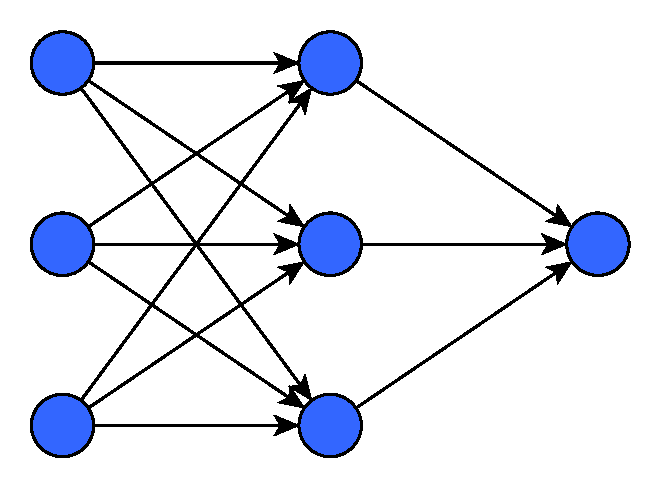
\includegraphics[width=.4\textwidth]{../img/neuralNetwork.pdf}
 	\end{tabular} 
	};
    \end{tikzpicture} 
    }
	{
	\begin{tikzpicture}
 %  \draw (0,0) rectangle (4,2);
%  \draw [rounded corners=5pt] (0,0) -- (0,2) -- (4,2) -- (4,0) -- (0,0);
  \node [ultra thick, draw = black, rounded corners] { 
 	 \begin{tabular}{c} 
 	 	Machine  \\ 
 	 	\hphantom{aaa}Learning\hphantom{aaa} \\
  		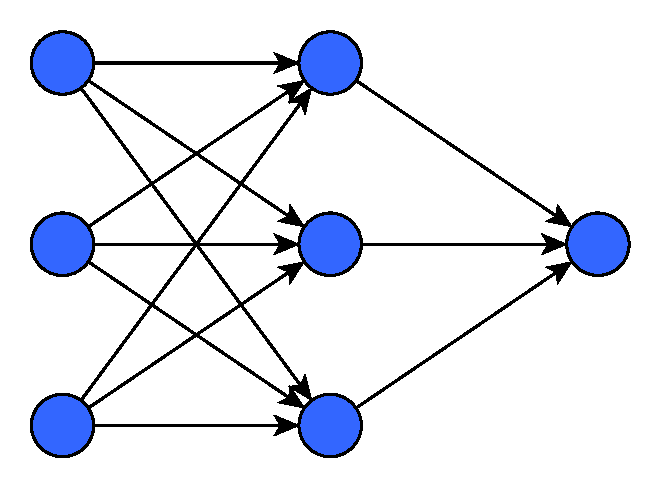
\includegraphics[width=.4\textwidth]{../img/neuralNetwork.pdf}
 	\end{tabular} 
	};
    \end{tikzpicture} 
	}    
 %    MAE: 0.4
      \end{center}
  \end{column}
  
\end{columns}

%\begin{columns}[t]
%\column{.3\textwidth}
%\begin{block}{Emoticon-Liste}
%\centering
%
\includegraphics[width=.31\textwidth]{../img/registry-book.pdf}
%\end{block}
%\column{.3\textwidth}
%\begin{block}{Wörterbuch}
%\centering
%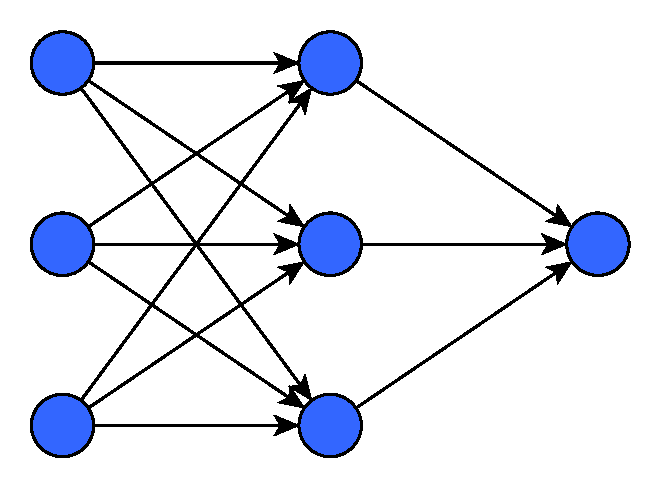
\includegraphics[width=.4\textwidth]{../img/neuralNetwork.pdf}
%\end{block}
%\column{.3\textwidth}
%\begin{block}{Machine Learning}
%\centering
%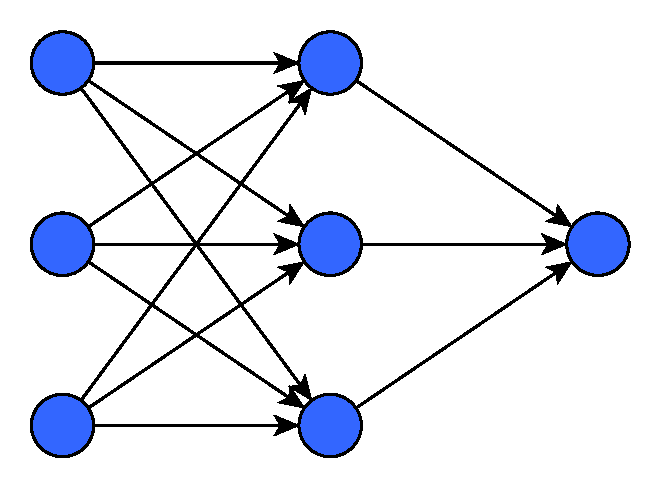
\includegraphics[width=.4\textwidth]{../img/neuralNetwork.pdf}
%\end{block}
%\end{columns}

\bigskip

\begin{itemize}
\item<1-> I love puppies \alt<1>{\color{SentiGreen}\textbf{:-)} }{:-)}
%
\item<2-3> I \alt<2>{\textcolor{SentiGreen}{\textbf{love}}}{love} puppies :-)
%
\item<3>  
\alt<3>{\textcolor{SentiLightRed}{\textbf{I}}}{I} 
\alt<3>{\textcolor{SentiGreen}{\textbf{love}}}{love} 
\alt<3>{\textcolor{SentiDarkGreen}{\textbf{puppies}}}{puppies} 
\alt<3>{\textcolor{SentiGreen}{\textbf{:-)}}}{:-)} 
%
\end{itemize}

\bigskip

\end{frame}

%%%%%%%%%%%%%%%%%%%%%%%%%%%%%%%%%%%%%%%%%%%%%%%%%%%%%
%%%%%%%%%%%%%%%%%%%%%%%%%%%%%%%%%%%%%%%%%%%%%%%%%%%%%
%%%%%%%%%%%%%%%%%%%%%%%%%%%%%%%%%%%%%%%%%%%%%%%%%%%%%
%%%%%%%%%%%%%%%%%%%%%%%%%%%%%%%%%%%%%%%%%%%%%%%%%%%%%

\begin{frame}{Module - Sentiment - Machine\,Learning\,mit\,Regression}

\begin{itemize}

\item Trainingsdaten:
\begin{itemize}
\item ``I love puppies''
\item ``I hate puppies''
%\item Sätze:
%\begin{itemize}
%\item I love puppies
%\item I hate puppies
%\end{itemize}

\pause

\item Merkmalsmatrix:
\item[]
\begin{tabular}{cccc|c}
I & love & hate & puppies & Sentiment \\
1 & 1 & 0 & 1 & \textcolor{SentiGreen}{\(+1\)} \\
1 & 0 & 1 & 1 & \textcolor{red}{\(-1\)} \\
\end{tabular}
\end{itemize}

\pause

\item Regressionsmodell:
\item[]
\begin{tabular}{cccc}
I & \textcolor{SentiGreen}{love} & \textcolor{red}{hate} & puppies \\
0 & \textcolor{SentiGreen}{\(+1\)} & \textcolor{red}{\(-1\)} & 0 \\
\end{tabular}

\pause

\item Neue Tweets: z. B. ``I love kitties''
\item[]
\begin{tabular}{ccccc}
I & & \alt<5>{\textcolor{SentiGreen}{love}}{love} & kitties & \\

\pause

0 & + & \textcolor{SentiGreen}{1} &  & \textcolor{SentiGreen}{\(=1\)} \\
\end{tabular}

\end{itemize}

\end{frame}

%%%%%%%%%%%%%%%%%%%%%%%%%%%%%%%%%%%%%%%%%%%%%%%%%%%%%
%%%%%%%%%%%%%%%%%%%%%%%%%%%%%%%%%%%%%%%%%%%%%%%%%%%%%
%%%%%%%%%%%%%%%%%%%%%%%%%%%%%%%%%%%%%%%%%%%%%%%%%%%%%
%%%%%%%%%%%%%%%%%%%%%%%%%%%%%%%%%%%%%%%%%%%%%%%%%%%%%

\begin{frame}{Module - Sentiment - Architektur}

\begin{figure}[p]
\centering
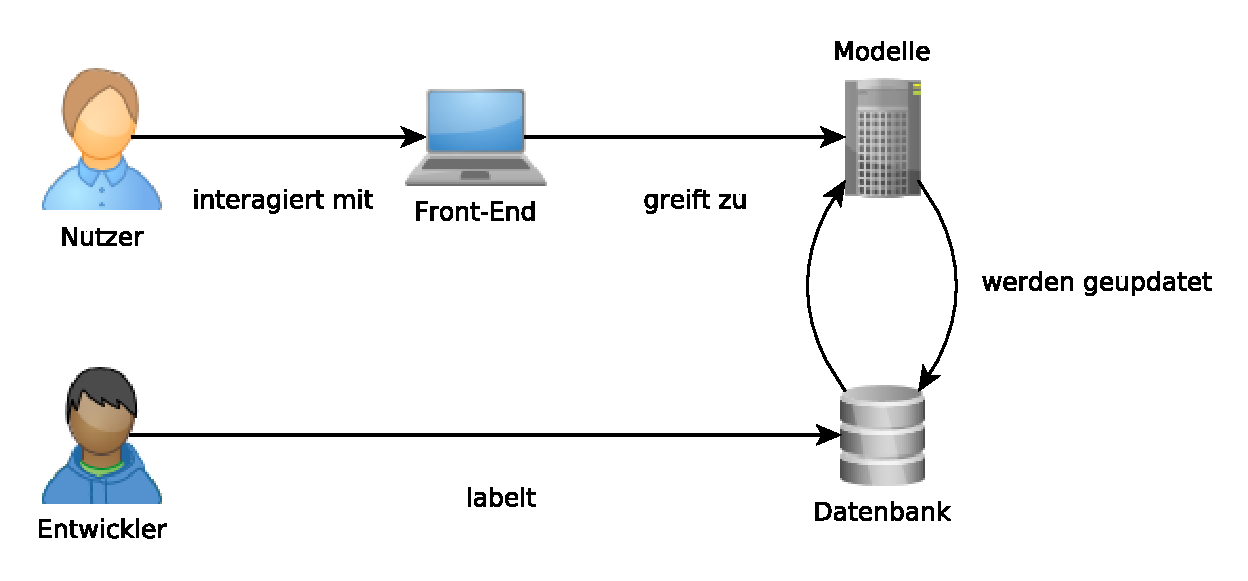
\includegraphics[scale=0.5]{../img/sentiment-architektur.pdf}
\end{figure}
\end{frame}

% Folie 4/4: Beschreiben, wie Sentiment-Werte dem Nutzer im Frontend dargestellt werden und wie Nutzer explorativ herausfinden kann, wie Wert zustande gekommen ist.
%%%%%%%%%%%%%%%%%%%%%%%%%%%%%%%%%%%%%%%%%%%%%%%%%%%%%
%%%%%%%%%%%%%%%%%%%%%%%%%%%%%%%%%%%%%%%%%%%%%%%%%%%%%
%%%%%%%%%%%%%%%%%%%%%%%%%%%%%%%%%%%%%%%%%%%%%%%%%%%%%
%%%%%%%%%%%%%%%%%%%%%%%%%%%%%%%%%%%%%%%%%%%%%%%%%%%%%

% \begin{frame}
% \frametitle{Module - Sentiment - Anzeige im Frontend}
% 
% 
% \begin{columns}
% \begin{column}{.49\textwidth}
% \begin{itemize}
% \item Diagramme mit Sentiment-Verteilung
% \item Filtern der Tweets nach Sentiment
% \item Einflussfaktoren auf Sentiment
% \item Trainingsdaten zu Einflussfaktoren
% \end{itemize}
%  \end{column}
% 
%  \begin{column}{.49\textwidth}
% \centering
% 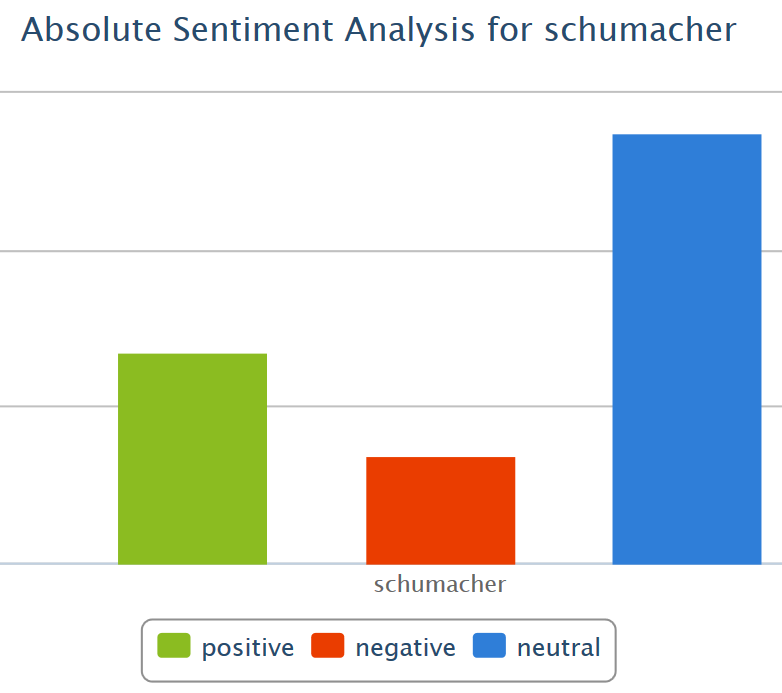
\includegraphics[height=.65\textheight]{../img/sentiment-overview1.png}
% % \\
% %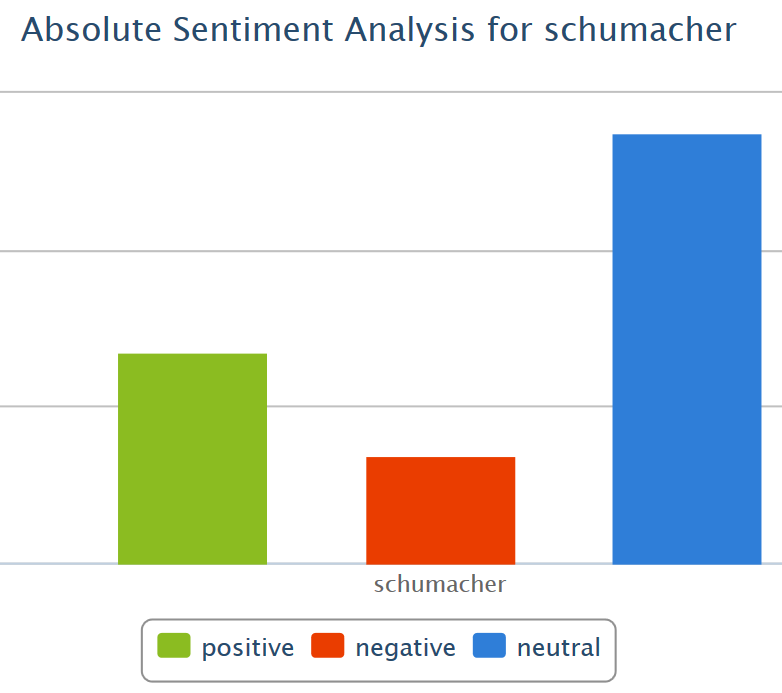
\includegraphics[height=.49\textheight]{../img/sentiment-overview1.png}
%  \end{column}
% 
% \end{columns}
% 
% \end{frame}
\subsection{News-Modul}
  \begin{frame}{Module - News - Datenquelle}
\begin{center}
\scalebox{0.8}{
\begin{tikzpicture}[scale=.6,database/.style={
      cylinder,
      cylinder uses custom fill,
      cylinder body fill=lblue,
      cylinder end fill=lblue,
      shape border rotate=90,
      aspect=0.25,
      align=center,
      draw
    }]
\definecolor{silver}{RGB}{158,158,169}
\definecolor{midgray}{rgb}{.35,.35,.35}
\definecolor{lightsilver}{RGB}{221,221,232}
\definecolor{lblue}{RGB}{210,220,250}
\definecolor{mblue}{RGB}{165,190,225}
\definecolor{dblue}{RGB}{0,70,117}
\definecolor{lgreen}{RGB}{200,245,185}
\definecolor{mgreen}{RGB}{190,225,165}
\definecolor{mred}{RGB}{225,190,165}
\definecolor{dgreen}{RGB}{40,135,40}
\definecolor{dred}{RGB}{135,40,40}
    
\node[ellipse,fill=mgreen,draw=black,align=center,font=\small, minimum height=1cm, minimum width= 2.9cm] (ne1) at (6, 0) {Google News};3
\node[ellipse,fill=mgreen,draw=black,align=center,font=\small, minimum height=1cm, minimum width= 2.9cm] (ne2) at (11.5, 0) {Bing Web};
\node[ellipse,fill=mgreen,draw=black,align=center,font=\small, minimum height=1cm, minimum width= 2.9cm] (ne3) at (17, 0) {Bing News};

\visible<2->{
\draw [decorate,thick,decoration={brace,amplitude=10pt,mirror,raise=4pt}]
(4,-1) -- (19,-1);
\node[single arrow, draw, fill=lightsilver, align=center, shape border rotate=270, minimum height=3cm,font=\small](parse) at (11.5, -4) {\ \\ collect and\\ parse RSS};
}

\visible<3->{
\node[database, minimum width=2cm, minimum height=1.5cm, font=\small] (db) at (0,0) {MySQL \\ DB};
\node[single arrow, draw, fill=lightsilver, align=center, shape border rotate=270, minimum height=3cm,font=\small](parse) at (0, -4.2) {\ \\ collect\\ tweets};
}

\visible<4->{
\node[fill=lblue,draw=black,align=center,font=\small, minimum height=1cm, minimum width= 10cm] (ne3) at (5.75, -9) {compare news and tweets to find relevant news};
\node[single arrow, draw, fill=mred, align=center, shape border rotate=0,font=\small, minimum height=2.6cm, minimum width=1.3cm](parse) at (17,-9) {top news};
}

\end{tikzpicture}
}
\end{center}
\end{frame}
\begin{frame}{Module - News - Peaksuche}
\begin{center}
\scalebox{0.75}{
\begin{tikzpicture}[point/.style={
    thick,
    draw=dgreen,
    cross out,
    inner sep=0pt,
    minimum width=4pt,
    minimum height=4pt,
}]
\definecolor{silver}{RGB}{158,158,169}
\definecolor{midgray}{rgb}{.35,.35,.35}
\definecolor{lightsilver}{RGB}{221,221,232}
\definecolor{lblue}{RGB}{210,220,250}
\definecolor{mblue}{RGB}{165,190,225}
\definecolor{dblue}{RGB}{0,70,117}
\definecolor{lgreen}{RGB}{200,245,185}
\definecolor{mgreen}{RGB}{190,225,165}
\definecolor{mred}{RGB}{225,190,165}
\definecolor{dgreen}{RGB}{40,135,40}
\definecolor{dred}{RGB}{135,40,40}
    
\begin{scope}[shift={(0,0)},scale=.2]
\draw[-] (0,0.2) -- (1,1) -- (2,1.1) -- (3,0.5) -- (4,1.2) -- (5,0) -- (6,0.2) -- (7,1) -- (8,1.1) -- (9,4.5) -- (10,2.2) -- (11,2) -- (12,3.2) -- (13,1) -- (14,1.1) -- (15,0.5) -- (16,1.2) -- (17,0) -- (18,0.2) -- (19,1) -- (20,1.1) -- (21,0.5) -- (22,1.2) -- (23,0) -- (24,0.2) -- (25,1) -- (26,1.7) -- (27,0.5) -- (28,1.2) -- (29,0) -- (30,4.2);
\draw[->,semithick,>=stealth'] (-1.3,-1) -- (31,-1);
\draw[->,semithick,>=stealth'] (-1,-1.3) -- (-1,5);
\visible<6->{
\node[point] at (9,4.5) {};
\node[point] at (30,4.2) {};
}
\node[draw=none,silver,font=\scriptsize] at (-1,6) {\#tweets};
\node[draw=none,silver,font=\scriptsize] at (33,-1) {time};
\end{scope}

\visible<2->{
\begin{scope}[shift={(2,-3)},scale=.2]
\draw[-,silver] (0,0.2) -- (1,1) -- (2,1.1) -- (3,0.5) -- (4,1.2) -- (5,0) -- (6,0.2) -- (7,1) -- (8,1.1) -- (9,4.5) -- (10,2.2) -- (11,2) -- (12,3.2) -- (13,1) -- (14,1.1) -- (15,0.5) -- (16,1.2) -- (17,0) -- (18,0.2) -- (19,1) -- (20,1.1) -- (21,0.5) -- (22,1.2) -- (23,0) -- (24,0.2) -- (25,1) -- (26,1.7) -- (27,0.5) -- (28,1.2) -- (29,0) -- (30,4.2);
\draw[-] (2,1.1) -- (4,1.2) -- (8,1.1) -- (9,4.5) -- (12,3.2) -- (16,1.2) -- (20,1.1) -- (22,1.2) -- (26,1.7) -- (28,1.2) -- (30,4.2);
\node[font=\tiny] at (2,1.1) {\textbullet};
\node[font=\tiny] at (4,1.2) {\textbullet};
\node[font=\tiny] at (8,1.1) {\textbullet};
\node[font=\tiny] at (9,4.5) {\textbullet};
\node[font=\tiny] at (12,3.2) {\textbullet};
\node[font=\tiny] at (16,1.2) {\textbullet};
\node[font=\tiny] at (20,1.1) {\textbullet};
\node[font=\tiny] at (22,1.2) {\textbullet};
\node[font=\tiny] at (26,1.7) {\textbullet};
\node[font=\tiny] at (28,1.2) {\textbullet};
\node[font=\tiny] at (30,4.2) {\textbullet};
\visible<3->{
\draw[-,dashed,semithick,dred] (-0.5,2.5) -- (30.5,2.5);
}
\draw[->,semithick,>=stealth'] (-1.3,-1) -- (31,-1);
\draw[->,semithick,>=stealth'] (-1,-1.3) -- (-1,5);
\node[draw=none,silver,font=\scriptsize] at (-1,6) {\#tweets};
\node[draw=none,silver,font=\scriptsize] at (33,-1) {time};
\end{scope}
}

\visible<4->{
\begin{scope}[shift={(4,-6)},scale=.2]
\draw[-,silver] (2,1.1) -- (4,1.2) -- (8,1.1) -- (9,4.5) -- (12,3.2) -- (16,1.2) -- (20,1.1) -- (22,1.2) -- (26,1.7) -- (28,1.2) -- (30,4.2);
\visible<4>{
\draw[-]  (9,4.5) -- (12,3.2);
\node[font=\tiny] at (9,4.5) {\textbullet};
\node[font=\tiny] at (12,3.2) {\textbullet};
\node[font=\tiny] at (30,4.2) {\textbullet};
}
\visible<5->{
\node[font=\tiny,silver] at (9,4.5) {\textbullet};
\node[font=\tiny,silver] at (12,3.2) {\textbullet};
\node[font=\tiny,silver] at (30,4.2) {\textbullet};
\node[point] at (9,4.5) {};
\node[point] at (30,4.2) {};
}
\draw[-,dashed,semithick,mred] (-0.5,2.5) -- (30.5,2.5);
\draw[->,semithick,>=stealth'] (-1.3,-1) -- (31,-1);
\draw[->,semithick,>=stealth'] (-1,-1.3) -- (-1,5);
\node[draw=none,silver,font=\scriptsize] at (-1,6) {\#tweets};
\node[draw=none,silver,font=\scriptsize] at (33,-1) {time};
\end{scope}
}black

\end{tikzpicture}
}
\end{center}
\end{frame}
\section{Ausblick und Organisation}
  \begin{frame}{Ausblick}
Was wäre noch möglich gewesen? Was wurde nicht umgesetzt?
\\
\begin{itemize}
    \item Kino-Modul
    \item Heatmap über Landkarte
    \item Prognosemöglichkeiten
    \item weitere Performance-Optimierungen
    \item ...
\end{itemize}
\end{frame}
\begin{frame}{Vorgehen: Scrum ... but}
Scrum:
\begin{itemize}
    \item Planning Poker, Definition of Done
    \item Priorisierung durch Kunden
    \item Kundentreffen
    \item selbstorganisierendes Team
\end{itemize}
But:
\begin{itemize}
    \item Daily Scrum
    \item wöchentlich wechselnde Scrum Master
    \item Feature und Code Freeze
\end{itemize}
\end{frame}

  \begin{frame}{}
\begin{center}\huge{Vielen Dank f\"ur Ihre Aufmerksamkeit!}
\end{center}
\end{frame}


\begin{frame}{TMetrics}

% \large{
\textbf{Datenanalyse} auf \textbf{Twitterbeitr\"agen}
zur Erkennung und visuellen Darstellung von Meinungstrends
\begin{itemize}
 \item \textbf{Machine Learning}
 \item \textbf{Clustering}
 \item \textbf{Sentiment-Analyse}
\end{itemize}

% unter Zuhilfenahme von \textbf{Machine Learning}}\\
% (\textbf{Clustering} und \textbf{Sentiment-Analyse})\\

\begin{center}
\vspace{.5cm}
\scalebox{0.45}{
\begin{tikzpicture}[scale=.6,opacity=0.7,database/.style={
      cylinder,
      cylinder uses custom fill,
      cylinder body fill=lblue,
      cylinder end fill=lblue,
      shape border rotate=90,
      aspect=0.25,
      align=center,
      draw
    }]
\definecolor{silver}{RGB}{158,158,169}
\definecolor{midgray}{rgb}{.35,.35,.35}
\definecolor{lightsilver}{RGB}{221,221,232}
\definecolor{lblue}{RGB}{210,220,250}
\definecolor{mblue}{RGB}{165,190,225}
\definecolor{dblue}{RGB}{0,70,117}
\definecolor{lgreen}{RGB}{200,245,185}
\definecolor{mgreen}{RGB}{190,225,165}
\definecolor{mred}{RGB}{225,190,165}
\definecolor{dgreen}{RGB}{40,135,40}
\definecolor{dred}{RGB}{135,40,40}
    

\node[fill=mred,draw=black,font=\small, minimum height=1cm, minimum width= 2.5cm] (fe) at (0, -10.5) {{JS Frontend}};
\node[ellipse,fill=mblue,draw=black,font=\small, minimum height=1cm, minimum width= 2.5cm] (tw) at (13, 0) {Twitter};

\node[database, minimum width=2cm, minimum height=1.5cm, font=\small] (db) at (0,0) {MySQL \\ DB};
\node[fill=lblue,draw=black,font=\small, minimum height=1cm, minimum width= 2.5cm,align=center] (rs) at (0, -3) {Restservice \\ Tomcat};
\node[fill=lblue,draw=black,font=\small, minimum height=1cm, minimum width= 2.5cm] (de) at (5.5, 0) {Deamon};
\draw[->,semithick,>=stealth',shorten >=1pt] (tw) -- (de) node[midway,above,font=\scriptsize] {Twitter4J};
\draw[<->,semithick,>=stealth',shorten >=1pt,shorten <=1pt] (de) -- (db) node[midway,above,font=\scriptsize] {JDBC};
\draw[<->,semithick,>=stealth',shorten >=1pt,shorten <=1pt] (db) -- (rs) node[midway,left,font=\scriptsize] {JDBC};


\node[fill=lblue,draw=black,font=\small, minimum height=1cm, minimum width= 2.5cm,align=center] (ap) at (0, -6) {HTTP Apache};

\draw[->,semithick,>=stealth',shorten >=1pt] ([xshift=-0.5cm]ap.south) -- ([xshift=-0.5cm,yshift=1.5cm]fe.north) node[midway,left,align=right,font=\scriptsize] {Frontend Code};
\draw[<-,semithick,>=stealth',shorten <=1pt] ([xshift=0.5cm]ap.south) -- ([xshift=0.5cm]fe.north) node[midway,right,align=left,font=\scriptsize] {HTTP Requests};
\draw[->,semithick,>=stealth',shorten >=1pt] ([xshift=-0.25cm]rs.south) -- ([xshift=-0.25cm]ap.north) node[midway,left,font=\scriptsize] {Replies (JSON)};
\draw[<-,semithick,>=stealth',shorten <=1pt] ([xshift=0.25cm]rs.south) -- ([xshift=0.25cm]ap.north) node[midway,right,align=left,font=\scriptsize] {HTTP Requests};
\draw[->,semithick,>=stealth',shorten >=1pt] ([xshift=0cm]ap.south) -- ([xshift=0cm]fe.north) node[midway,left,align=right,font=\scriptsize] {\ \\ \ \\ Replies (JSON)};


\draw[<-,semithick,>=stealth',shorten <=1pt] (rs) -- (de) node[midway,right,font=\scriptsize] {SentimentModel};

\node[ellipse,fill=mgreen,draw=black,align=center,font=\small, minimum height=1cm, minimum width= 2.5cm] (ne) at (13, -3) {Google News \\ Bing Web \\ Bing News};
\draw[<-,semithick,>=stealth',shorten <=1pt] (rs) -- (ne) node[midway,above,font=\scriptsize] {RSS Feeds};



\end{tikzpicture}
}
\end{center}
\end{frame}
\section{Demonstration}
%   \begin{frame}{Suchbegriffsplitting}
	\begin{itemize}
		\item Teilweise riesige Anzahl von Tweets in kurzer Zeit % (Terroranschlag, Tod einer bekannten Person etc.)
		\item Idee: Mehrere Profile suchen zu \emph{einem} Begriff parallel
		\item Aber: Die Twitter-API bietet \emph{keine} Möglichkeit, Tweets Zeitgenau zu liefern. Man kann lediglich bis zu einem bestimmten Tweet suchen
	\end{itemize}
\end{frame}

\begin{frame}{Speicherprobleme}
	\begin{itemize}
		\item Der Daemon hat großen Datenmengen(Tweets) im RAM
		\item Daten nicht schnell genug in DB $\Rightarrow$ Speicher voll
		\item Kein Speicher $\Rightarrow$ \texttt{OutOfMemoryError} und der Thread stirbt
	\end{itemize}
\end{frame}

\begin{frame}{Multi-Threading}
	\begin{itemize}
		\item Größte Gefahren: Deadlocks, Inkonsistenzen etc.
		\item Beispiel: Exception innerhalb eines Mutex $\Rightarrow$ Deadlock
		\item Erst die Struktur entwickeln, dann Coden
	\end{itemize}
\end{frame}
  
%   \begin{frame}[allowframebreaks]{Literatur}
 

\begin{thebibliography}{10}
% \bibitem{Goldbach1742}[Goldbach, 1742]
% Christian Goldbach.
% \newblock A problem we should try to solve before the ISPN ’43 deadline,
% \newblock \emph{Letter to Leonhard Euler}, 1742.
\setbeamertemplate{bibliography item}[book]
\bibitem{} B. Preim, D. Bartz
\newblock Visualization in Medicine. 
\newblock \emph{Morgan Kaufmann, 2007}

\bibitem{} K. Engel, M. Hadwiger, J. Kniss, C. Rezk-Salama, D. Weiskopf
\newblock Real-Time Volume Graphics
\newblock \emph{A K Peters; 1 edition, 2006}
 
 \setbeamertemplate{bibliography item}[article]
 \bibitem{} G. Kindlmann , James W. Durkin.
 \newblock Semi-automatic generation of transfer functions for direct volume rendering. 
 \newblock \emph{Proceedings of the 1998 IEEE symposium on Volume visualization. ACM, 1998.}
%  
 \bibitem{} G. Kindlmann,  R. Whitaker,  T. Tasdizen, T. Möller
 \newblock Curvature-based transfer functions for direct volume rendering: Methods and applications.
 \newblock \emph{Visualization, 2003. VIS 2003. IEEE. IEEE, 2003.}
%  
 \bibitem{} J. Marks, P. Beardsley, B. Andalman, B. Freeman, S. Gibson, J.
Hodgins, T. Kang, B. Mirtich, H. Pfister, W. Ruml, J. Seims, and
S. M. Shieber
 \newblock Design galleries: A general approach to setting parameters for computer graphics and animation. 
 \newblock \emph{In Proceedings of SIGGRAPH 97, pages 389-400, Los Angeles, CA, 1997.}

\end{thebibliography} 

\end{frame}
\end{document}



